\documentclass[10pt,a4paper,oneside]{book}

% course info (for title)
\newcommand{\courseid}{PHYS 410}
\newcommand{\coursetitle}{Classical Mechanics}
\newcommand{\semester}{Fall 2024}
\newcommand{\credit}{Adapted from 
    \textit{Classical Mechanics} by John R. Taylor.}  

\usepackage[utf8]{inputenc}
\usepackage[margin=1.0in]{geometry}
\usepackage{amsmath}
\usepackage{amsfonts}
\usepackage{amssymb}
\usepackage{enumitem}                       % custom enum labels
\usepackage{parskip}                        % add vertical paragraph space
\usepackage{tocloft}						% modify toc position
\usepackage{xr}								% cross-references
\usepackage{mathtools}						% Aboxed
\usepackage{empheq}							% box multiple lines
\usepackage{upgreek}
\usepackage{siunitx}
\usepackage{chemformula}
\usepackage{esint}							% oiint
\usepackage{cancel}
\usepackage{bm}
\usepackage{physics}
\usepackage[framemethod=TikZ]{mdframed}     % graphics and framed envs
\usepackage[hang,flushmargin]{footmisc}		% remove footnote indentation
\usepackage[hyperfootnotes=false,
					hidelinks]{hyperref}	% create clickable table of contents


\renewcommand{\familydefault}{\sfdefault}  	% sans serifs text
\setlength{\parindent}{0pt}                	% no paragraph indentation

\AtBeginDocument{\RenewCommandCopy\qty\SI} 
 
% region TITLES
\setbox0=\hbox{\Huge{\textbf{\textsf{\courseid: }}}}
\setlength{\cftbeforetoctitleskip}{0em}
\setlength{\cftaftertoctitleskip}{1em}
\renewcommand{\contentsname}{\hangindent=\wd0 \strut \courseid: \coursetitle \\ \medskip \LARGE{Isabelle, \semester}}

\let\footnoterule\relax
\newcommand\blfootnote[1]{%
  \begingroup
  \renewcommand\thefootnote{}\footnote{#1}%
  \addtocounter{footnote}{-1}%
  \endgroup
}

\usepackage{titlesec}
\titleformat{\chapter}{\Huge\normalfont\bfseries}{\thechapter}{1em}{}
\titlespacing*{\chapter}{0em}{0em}{2em}
% endregion

\let\oldphi = \phi
\let\phi = \varphi

% region COMMANDS
\newcommand{\bsm}[1]{\boldsymbol{#1}}
\newcommand{\ds}{\displaystyle}
\newcommand{\pfn}[1]{\textrm{#1}}	% enables new functions
\newcommand{\mbf}[1]{\mathbf{#1}}	% mathbf
\newcommand{\C}{\mathbb{C}}			% fancy C
\newcommand{\R}{\mathbb{R}}			% fancy R
\newcommand{\Q}{\mathbb{Q}}			% fancy Q
\newcommand{\Z}{\mathbb{Z}}			% fancy Z
\newcommand{\N}{\mathbb{N}}			% fancy N
\newcommand{\from}{\leftarrow}
\newcommand{\qed}{$\square$}
\newcommand{\xhat}{\mbf{\hat{x}}}
\newcommand{\yhat}{\mbf{\hat{y}}}
\newcommand{\zhat}{\mbf{\hat{z}}}
\newcommand{\phihat}{\bm{\hat{\phi}}}
\newcommand{\rhat}{\mbf{\hat{r}}}
\newcommand{\dotunit}[1]{\bm{\dot{\hat{#1}}}}
\newcommand{\ddotunit}[1]{\bm{\ddot{\hat{#1}}}}
\renewcommand{\it}[1]{\textit{#1}}
\renewcommand{\bf}[1]{\textbf{#1}}
\renewcommand\pmat[1]{\begin{pmatrix}#1\end{pmatrix}} 
\newcommand\vmat[1]{\begin{vmatrix}#1\end{vmatrix}}
\newcommand\bmat[1]{\begin{bmatrix}#1\end{bmatrix}}
\newcommand{\mcl}[1]{\mathcal{#1}}
\renewcommand{\L}{\mcl{L}}
\renewcommand{\H}{\mcl{H}}

% endregion

% region ENVIRONMENTS
\newcounter{theo}[chapter]\setcounter{theo}{0}
\newcommand{\numTheo}{\arabic{chapter}.\arabic{theo}}
\newcommand{\mdftheo}[3]{
	\mdfsetup{
		frametitle={
			\tikz[baseline=(current bounding box.east),outer sep=0pt]
			\node[anchor=east,rectangle,fill=#3]
			{\ifstrempty{#2}{\strut #1~\numTheo}{\strut #1~\numTheo:~#2}};
		},
		innertopmargin=4pt,linecolor=#3,linewidth=2pt,
		frametitleaboveskip=\dimexpr-\ht\strutbox\relax,
		skipabove=11pt,skipbelow=0pt
	}
}
\newcommand{\mdfnontheo}[3]{
	\mdfsetup{
		frametitle={
			\tikz[baseline=(current bounding box.east),outer sep=0pt]
			\node[anchor=east,rectangle,fill=#3]
			{\ifstrempty{#2}{\strut #1}{\strut #1:~#2}};
		},
		innertopmargin=4pt,linecolor=#3,linewidth=2pt,
		frametitleaboveskip=\dimexpr-\ht\strutbox\relax,
		skipabove=11pt,skipbelow=0pt
	}
}
\newcommand{\mdfproof}[1]{
	\mdfsetup{
		skipabove=11pt,skipbelow=0pt,
		innertopmargin=4pt,innerbottommargin=4pt,
		topline=false,rightline=false,
		linecolor=#1,linewidth=2pt
	}
}

\newenvironment{theorem}[1][]{
	\refstepcounter{theo}
	\mdftheo{Theorem}{#1}{red!25}
	\begin{mdframed}[]\relax
}{\end{mdframed}}

\newenvironment{lemma}[1][]{
	\refstepcounter{theo}
	\mdftheo{Lemma}{#1}{red!15}
	\begin{mdframed}[]\relax
}{\end{mdframed}}

\newenvironment{corollary}[1][]{
	\refstepcounter{theo}
	\mdftheo{Corollary}{#1}{red!15}
	\begin{mdframed}[]\relax
}{\end{mdframed}}

\newenvironment{definition}[1][]{
	\mdfnontheo{Definition}{#1}{blue!20}
	\begin{mdframed}[]\relax
}{\end{mdframed}}

\newenvironment{proof}[1][]{
	\mdfproof{black!15}
	\begin{mdframed}[]\relax
\textit{Proof. }}{\qed \end{mdframed}}

\newenvironment{example}[1][]{
	\mdfnontheo{Example}{#1}{yellow!40}
	\begin{mdframed}[]\relax
}{\end{mdframed}}

\newenvironment{summary}[1][]{
	\mdfnontheo{Summary}{#1}{green!70!black!30}
	\begin{mdframed}[]\relax
}{\end{mdframed}}
% endregion
\graphicspath{{figures/}}

\usepackage{subfiles}

\begin{document}
\tableofcontents
\blfootnote{* \credit}
\graphicspath{{figures/}}

\chapter{Newton's Laws of Motion}
\section{Space, Time, Mass, and Force}
Newton's laws of motion are formulated in terms of four crucial concepts: space, time, mass, and force. We will briefly review these 
concepts here. 

\subsection*{Space}
Every point $P$ of the three-dimensional space in which we live can be represented with a position vector $\bm{r}$ that specifies the distance and direction of $P$ from a chosen origin $O$. We can represent a position vector by expressing its components $(x,y,z)$ in the direction of three given perpendicular axes. One popular choice of axes is described by the unit vectors $\xhat$, $\yhat$, and $\zhat$, which have a length of one and point along the $x$, $y$, and $z$ axes. We can then write 
\begin{equation} \label{unit_vectors}
    \mbf{r} = x\xhat + y\yhat + z\zhat
\end{equation}
Some texts may use the equivalent notation of $\mbf{i}$, $\mbf{j}$, and $\mbf{k}$. Different authors have different preferences, so it will be helpful to get used to working with several notations.

We sometimes abbreviate (\ref{unit_vectors}) by simply writing
\begin{equation} \label{abb_vector}
    \mbf{r} = (x,y,z)
\end{equation}
When the choice of unit vectors is clear from the context. For most vectors, we will indicate the components of the vector with the subscripts $x$, $y$, and $z$. For instance, the velocity vector $\mbf{v}$ has components $v_x$, $v_y$, and $v_z$.

Sometimes, it become convenient to write vectors even more concisely using the summation sign $\sum$. In these cases, we will rename the unit vectors $\xhat$, $\yhat$, and $\zhat$ to $\mbf{e_1}$, $\mbf{e_2}$, and $\mbf{e_3}$ and we will rename the components $x$, $y$, and $z$ to $r_1$, $r_2$, and $r_3$. With this notation, we can write
\[ \mbf{r} = r_1\mbf{e_1} + r_2\mbf{e_2} + r_3\mbf{e_3} = \sum_{i=1}^3 r_i\mbf{e_i} \]

\subsection*{Time}
In classical mechanics, we view time as one universal parameter--that is, all objects will experience the flow of time at precisely the same rate. The theory of relativity states that this is not quite correct, which gives rise to phenomena such as length contraction and time dilation. However, for objects whose velocity is much less than the speed of light, these effects are negligible and we will ignore them.

\subsection*{Reference Frames}
Every time we wish to solve a problem in physics, we will have to choose a \it{reference frame}. Reference frames give a choice of spatial origin and axes, as well as an origin for time. Choosing an appropriate reference frame will simplify calculations for many problems, and is a skill that will be vital to build.

When choosing a reference frame, it will be important to note the difference between \it{inertial} reference frames and non-inertial ones. This is because Newton's laws of motion will only hold true in inertial reference frames. 

Any frame of reference that is accelerating or rotating relative to an inertial frame is non-inertial. Studying non-inertial frames will require more advanced techniques than we currently have, so we will focus solely on inertial frames for the time being.

\subsection*{Mass}
The mass of an object characterizes its inertia, or resistance to movement. An object with a large amount of mass, like a boulder, will be harder to accelerate than an object with less mass, like a marble.

\subsection*{Force}
Informally, we think of a force as a push or a pull on an object. This is a surprisingly useful starting point, as we are typically very conscious of the forces we exert on the world and the world exerts on us. Forces are vector quantities that can be represented as
\[ \mbf{F} = F_x\xhat + F_y\yhat + F_z\zhat \]
We can also represent the magnitude of a force with $F = \sqrt{F_x^2 + F_y^2 + F_z^2}$. 

\section{Newton's First and Second Laws; Inertial Frames}
Throughout this chapter, we will discuss Newton's laws as they apply to a \bf{point mass}. A point mass is a ficticious construct of an object with mass, but no size. Of course, all objects have some sort of size--but many objects are so small that treating them as a point mass will not cause any issues. Later, we will explore the mechanics of extended bodies by representing them as a collection of many point masses.

The first two of Newton's laws are easily stated and well-known.

\begin{theorem}[Newton's First Law]
    Newton's first law tells us that in the absence of forces, a particle moves with a constant velocity $\mbf{v}$.
\end{theorem}
\begin{theorem}[Newton's Second Law]
    Newton's second law tells us that the net force $\mbf{F}$ is equal to the product of its mass $m$ and its acceleration $\mbf{a}$:
    \[ \mbf{F} = m\mbf{a} \]
\end{theorem}
We will introduce the notation $\mbf{a} = \mbf{\dot v} =  \mbf{\ddot{r}}$, where each dot represents the operation of differentiation with respect to $t$. This means that we can also write $\mbf{F} = m\mbf{\ddot{r}}$.

Alternatively, we can write Newton's second law in terms of the particle's \bf{momentum}. Momentum is a vector quantity defined as
\[ \mbf{p} = m\mbf{v} \]
Thus, $\mbf{\dot p} = m\mbf{\dot v} = m\mbf{a}$, so we can state
\[ \mbf{F} = \mbf{\dot p} \]
\subsection*{Differential Equations}
In the form $\mbf{F} = m\mbf{\ddot r}$, Newton's second law is a second order differential equation (or perhaps a higher order one if $\mbf{F}$ depends on higher derivatives of $\mbf{r}$) describing the position $\mbf{r}(t)$ of the particle. 

This representation gives us a few key insights about a particle. These insights draw from the theory of differential equations, and may be explained in more detail in a text dedicated to that theory.

\begin{enumerate}
    \item If the force can be described as a piecewise-continuous function of $\mbf{r}$ and its derivatives and $t$, then a family of functions describing posisble positions $\mbf{r}(t)$ can be found.
    \item The family of position functions can be narrowed down to one unique position function using a pair initial conditions $\mbf{r}(t_0) = \mbf{r_0}$ and $\mbf{r}'(t_0) = \mbf{r_0'}$.
    \item If $\mbf{F}$ depends on higher order derivatives of $\mbf{r}$, more initial conditions will be required as the equation will increase in order.
\end{enumerate}

\subsection*{Inertial Frames}
Previously, we said that Newton's laws do not hold up in non-inertial reference frames. To see this, consider some frame $\mathcal{S}$ where Newton's laws hold. $\mathcal{S}$ is then an inertial frame. If we consider some other frame $\mathcal{S}'$ that is moving at a constant velocity in a straight line relative to $\mathcal{S}$, we'll notice that any object that isn't accelerating in $\mathcal{S}$ is also not accelerating in $\mathcal{S}'$. Therefore the law of inertia holds in $\mathcal{S}'$ and so $\mathcal{S}'$ is also inertial. 

If we consider a third frame $\mathcal{S}''$ that is accelerating relative to $\mathcal{S}$, then any object moving at a constant velocity in $\mathcal{S}$ is accelerating in $\mathcal{S}''$. The amount of acceleration it has is equal to the amount $\mathcal{S}''$ is accelerating relative to $\mathcal{S}$, but in the opposite direction.

For the time being, we will just consider the mechanics of objects in inertial reference frames, but we will explore noninertial frames in more detail later on.

\subsection*{Validity of the First Two Laws}
Since the advent of relativity and quantum mechanics, we have known that Newton's laws are not universally valid. However, there are still many cases where they are. Even as the speed of objects approaches the speed of light $c$, the law of inertia remains completely valid. But in these cases, the second law $\mbf{F} = m\mbf{a}$ is no longer valid and we must instead use $\mbf{F} = \mbf{\dot p}$.

The main takewaway here is that for most scenarios we will be working with, the first two laws are completely valid.
\section{Newton's Third Law}
Every force that is exerted on an object will always involve a second force--the reaction force back onto the object that exerts the force. When you push on a wall, the wall pushes back (otherwise you'd just fall right through). 

So forces come in pairs. We will introduce a new notation $\mbf{F}_{21}$ to denote the force exerted on object 2 by object 1. Similarly, $\mbf{F}_{12}$ denotes the force exerted on object 1 by object 2. With this notation, we can express Newton's third law quite compactly. 

\begin{theorem}[Newton's Third Law]
    If object 1 exerts a force $\mbf{F}_{21}$ on object 2, then object 2 exerts a reaction force $\mbf{F}_{12}$ on object 1 given by
    \begin{equation}
        \mbf{F}_{12} = -\mbf{F}_{21}
    \end{equation}
\end{theorem}
In the special case where $\mbf{F}_{12}$ an $\mbf{F}_{21}$ act parallel to the line connecting object 1 and object 2, we call them \bf{central forces}. Many of the most common forces we encounter are central forces: gravity, the electrostatic force, etc.

Newton's third law has a nice connection with the law of conservation of momentum. Imagine two objects that exert forces $\mbf{F}_{12}$ and $\mbf{F}_{21}$ on each other, and perhaps have some other external forces acting on them. The net force on each object can be expressed as 
\[ \mbf{F}_1 = \mbf{F}_{12} + \mbf{F}^{\text{ext}}_1 \]
and
\[ \mbf{F}_2 = \mbf{F}_{21} + \mbf{F}^{\text{ext}}_2 \]
which, by Newton's second law, tells us that $\mbf{\dot p}_1 = \mbf{F}_{12} + \mbf{F}^{\text{ext}}_1$ and $\mbf{\dot p}_2 = \mbf{F}_{21} + \mbf{F}^{\text{ext}}_2$. The total momentum of the system is the sum of each individual objects' momentum $\mbf{P} = \mbf{p}_1 + \mbf{p}_2$. Thus
\begin{align*}
    \mbf{\dot P} &= \mbf{\dot p}_1 + \mbf{\dot p}_2 \\
    &= \mbf{F}_{12} + \mbf{F}^{\text{ext}}_1 + \mbf{F}_{21} + \mbf{F}^{\text{ext}}_2
\end{align*}
By Newton's third law, $\mbf{F}_{12} = -\mbf{F}_{21}$ so they cancel out, simply leaving us with
\[ \mbf{\dot P} = \mbf{F}^{\text{ext}}_1 + \mbf{F}^{\text{ext}}_2 \equiv \mbf{F}^{\text{ext}}\]
This leads to a critical observation for our two-particle system--if the net external force on the system is zero, then the total momentum of the system is constant.

We will now show that the same result holds for any $N$-particle system.

Consider a system of $N$ particles where the net force on particle $i$ is given by
\[ \mbf{F}_i = \mbf{\dot p}_i = \mbf{F}^{\text{ext}}_i + \sum_{j \neq i} \mbf{F}_{ij}\]
The sum rate of change of the momentum of the system is the sum of each of these net forces,
\begin{align*}
    \mbf{\dot P} &= \sum_{i} \mbf{\dot p}_i  \\
    &= \sum_{i} \pqty{ \mbf{F}^{\text{ext}}_i + \sum_{j \neq i} \mbf{F}_{ij}} \\
    &= \mbf{F}^{\text{ext}} + \sum_{i}\sum_{j \neq i} \mbf{F}_{ij}
\end{align*}
The second term consists of $N+(N-1)$ terms and can be split into $n(n-1)/2$ pairs of forces that cancel with each other. We can show this mathematically with a manipulation of the summation. 
\[\sum_{i}\sum_{j \neq i} \mbf{F}_{ij} = \sum_{i}\sum_{j < i}(\mbf{F}_{ij} + \mbf{F}_{ji}) = 0 \]
Therefore the total rate of change of momentum on the system is given by
\[ \mbf{\dot P} = \mbf{F}^{\text{ext}} \]
Now we can make a more general statement of the principle of conservation of momentum.
\begin{theorem}[Conservation of Momentum]
    If the net external force $\mbf{F}^{\text{ext}}$ on an $N$-particle system is zero, then the system's total momentum is constant.
\end{theorem}
\subsection*{Validity of Newton's Third Law}
Similar to Newton's first and second laws, the third law is not universally applicable. As speeds of objects approach $c$, the third law cannot hold because the time-dependent action and reaction forces $\mbf{F}_1(t)$ and $\mbf{F}_2(t)$ for two objects differ depending on the speed of the observer, even if their frame of reference is inertial.

There is also an example of a quite common force where Newton's third law doesn't hold: the magnetic force between two moving point charges. 

Consider two positively charged particles, one with charge $q_1$ moving in the $\xhat$ direction and one with charge $q_2$ moving in the $\yhat$ direction. As per the Biot-Savart law, the direction of the magnetic field $\mbf{B_2}$ created by $q_1$ at the location of $q_2$ is given by 
\[ \mbf{B_2} \propto \mbf{\dot r}_1 \times \mbf{\hat d} \]
where $\mbf{d}$ is the displacement vector between $q_1$ and $q_2$. $\mbf{\dot r}_1$ is in the $\xhat$ direction and $\mbf{d}$ is in the $\xhat$-$\yhat$ plane, so $\mbf{B_2}$ lies one the $\zhat$ axis.

A similar argument shows that $\mbf{B_1}$ is in the \textit{negative} $\zhat$ direction. 

Then, the magnetic component of the Lorentz force for each particle is given by
\begin{align*}
    \mbf{F}_{B,1} = \mbf{F}_{12} &= q_1\mbf{\dot r_1}\times \mbf{B_1}\\
    &= q_1\dot r_1 B_1 (\xhat \times \zhat) \\
    &= q_1\dot r_1B_1 \yhat
\end{align*}
and
\begin{align*}
    \mbf{F}_{B,2} = \mbf{F}_{21} &= q_2\mbf{\dot r_2}\times \mbf{B_2}\\
    &= q_2\dot r_2 B_2 (\yhat \times -\zhat) \\
    &= q_1\dot r_2B_2 \xhat 
\end{align*}
clearly, these forces do not act in opposite directions, violating Newton's third law.

Because we have shown that the statement of conservation of momentum is equivalent to the statement of Newton's third law, this result seem to imply that the magnetic force does not obey the conservation of momentum.

This error comes from the fact that the introductory physics view of electromagnetism does not portray the full picture of electromagnetic interactions. In fact, the lost momentum in the two particles is actually stored within the electromagnetic fields themselves.

It can be shown that for a particles moving with speeds $v_1$ and $v_2$, the magnitude of the electric force between the particles is greater than or equal to $v_1v_2/c^2$ times the magnetic force. Therefore the magnetic force can be taken to be negligible compared to the electric force and the lost mechanical momentum can be safely disregarded for low speeds.

\section{Newton's Second Law in Cartesian Coordinates}
We will now see how we can use the relationship $\mbf{F} = m\mbf{\ddot r}$ to solve for the motion of objects. This relationship can be split into a separate equation for each direction with the expansion
\[ \mbf{F} = F_x\xhat + F_y\yhat + F_z\zhat \]
and
\[ \mbf{\ddot r} = \ddot x\xhat + \ddot y\yhat + \ddot z\zhat \]
thus giving the three equations of motion
\[ F_x = m\ddot x \quad F_y = m\ddot y \quad F_z = m\ddot z \]
Generally, when we solve a problem of this form we will qualitatively analyze the situation to determine each force present on the object, and then solve the corresponding system of differential equations. 
\begin{example}[Inclined Plane] \label{inclined}
    A block of mass $m$ begins at rest on an inline with a coefficient of friction $\mu$ that rests at an angle $\theta$ above the horizontal floor. Determine an expression for how far the block will slide during a certain time $t$.
    
    \begin{minipage}{0.48\textwidth}
        As with any mechanics problem, we will begin by defining our frame of reference. We will choose the origin point of our coordinate system to be at the initial position of the block, and we will define the $\xhat$ direction as going down the slope of the incline, and the $\yhat$ direction as protruding upward from the incline at a $90$ degree angle. We will define the $\zhat$ direction as the direction given by $\xhat \times \yhat$, but this will prove to be irrelevant as no forces act in that direction.
    \end{minipage}
    \begin{minipage}{0.48\textwidth}
        \parbox{\textwidth}{
            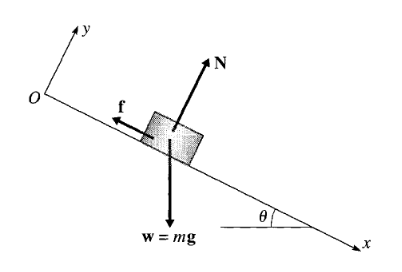
\includegraphics[width=\textwidth]{blockSlidingExample.png}
        }
    \end{minipage}
    
    This is a particularly useful frame of reference because it ensures that the friction force and normal force both lie in the direction of one of our basis vectors.

    From the figure and a relatively simple exercise in trigonometry, we can determine the directions of each force. The frictional force $\mbf{f}$ acts purely in the $-\xhat$ direction, the normal force $\mbf{N}$ acts purely in the $\yhat$ direction, and the weight force $\mbf{w}$ has components in both directions, with relative magnitudes given by
    \[ \mbf{w} = w\sin\theta\xhat - w\cos\theta\yhat\]
    So the net force on the object is given by
    \[ \mbf{F} = (mg\sin\theta - \mu N)\xhat + (N - mg\cos\theta)\yhat\]
    Because the block is not accelerating at all in the $\yhat$ direction, the component of $\mbf{F}$ in the $\yhat$ direction must be zero, telling us that
    \[ N - mg\cos\theta = 0\]
    or $N = mg\cos\theta$. Substituting this back into the expression for $F_x$, we get
    \[ F_x = mg\sin\theta - \mu mg \cos\theta \]
    By Newton's Second Law, this gives us the differential equation
    \[ \ddot x = g\sin\theta - \mu g\cos \theta \]
    Which can be solved by integrating twice to find 
    \[ x(t) = \frac{1}{2}g(\sin\theta-\mu\cos\theta)t^2 \]
    Both constants of integration are simply zero due to the prescribed initial condition $x(0)=x'(0) = 0$.
\end{example}
\section{Two Dimensional Polar Coordinates}
Cartesian coordinates are very simple to work with, but there are many cases where polar coordinates prove more effective. Recall from introductory Calculus that polar coordinates can be related to recangular coordinates with
\[ 
\begin{rcases}
    x = r\cos\phi \\
    y = r\sin\phi
\end{rcases} \longleftrightarrow \begin{cases}
    r = \sqrt{x^2+y^2} \\
    \tan\phi = y/x
\end{cases}
\]
In physics, it is common to use $\phi$ as the polar angle rather than $\theta$. One thing to note is the possible ambiguity in the expression $\tan\phi = y/x$. Because $\tan(y/x) = \tan(-y/-x)$ and $\tan(-y/x) = \tan(y/-x)$, we will have to be careful to find the correct quadrant of $\phi$ when converting from rectangular to polar coordinates.

Just as in rectangular coordinates, we introduce two unit vectors $\rhat$ and $\phihat$. $\rhat$ is defined as the direction we move as $r$ increases while $\phi$ is held constant, and $\phihat$ is defined as the direction we move as $\phi$ increases while $r$ is held constant. 

These two unit vectors form an orthonormal basis for $\R^2$ and we can expand forces in terms of them as
\[ \mbf{F} = F_r\rhat + F_\phi \phihat\]
We can also note that $\mbf{r} = r\rhat$. Initially, it seems odd that the position vector has no explicit dependence on $\phi$. The dependence actually originates from the unit vector $\rhat$. Unlike the unit vectors in cartesian coordinates, the polar unit vectors are not constant, and depend on the state of the system. 

This revelation complicates our expression of Newton's Second Law in polar, as 
\[ \ddot r = \dv[2]{t}(r\rhat) \neq r\mbf{\ddot{\hat r}}\]
To resolve this, we'll draw a picture.

Suppose a particle is at a position $r\rhat + \phi\phihat$ at time $t_1$ and a position $(r + \Delta r)(\rhat + \Delta\rhat) + (\phi + \Delta \phi)(\phihat + \Delta\phihat)$ at $t_2 = t_1 + \Delta t$. Notice from the below figure that $\Delta \rhat$ is not dependent on $\Delta r$, so we will assume it is zero, so
\[ \mbf{r}(t_2) = r(\rhat + \Delta \rhat) + (\phi + \Delta \phi)(\phihat + \Delta \phihat)\]
\begin{figure}[h!]
    \centering
    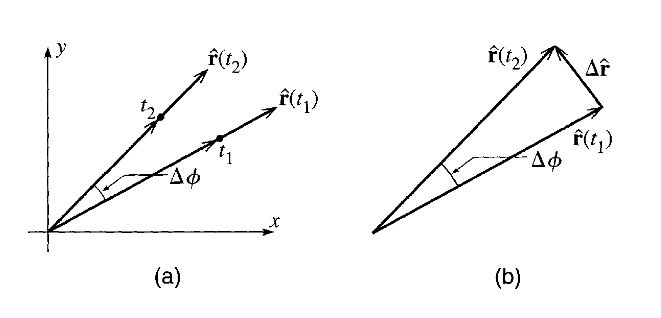
\includegraphics[width=0.65\linewidth]{polarDerivatives.png}
    \caption{\bf{(a)} Unless the particle is moving completely radially, the $\rhat$ vectors differ at $t=t_1$ and $t=t_2$. \bf{(b)} The change $\Delta \rhat$ is given by the pictured triangle.}
    \label{fig:polarDerivatives}
\end{figure}

As shown in part \bf{(b)} of the above figure, $\Delta \rhat$ is described by the triangle with an angle $\Delta \phi$ and two sidelengths of length one (since each $\rhat$ satisfies $\norm{\rhat} = 1$). We can use some geometry to find $\Delta \rhat$. The law of cosines tells us that
\[ \norm{\Delta \rhat} = \sqrt{2 - 2\cos\Delta\phi}\]
With the small-angle approximation 
\begin{equation} \label{small_angle_polar_unit}
    \cos\Delta\phi \approx 1 - \frac{\Delta \phi ^2}{2}
\end{equation}
we obtain
\[ \norm{\Delta\rhat} \approx \abs{\Delta\phi} \]
We can also see from ($\ref{fig:polarDerivatives}$b) that $\Delta \rhat$ points in the direction of $\phihat(t_1)$. Therefore,
\[ \Delta \rhat \approx \Delta \phi \phihat(t_1) \]
or
\[ \frac{\Delta \rhat}{\Delta t} \approx \frac{\Delta \phi}{\Delta t} \phihat(t_1) \]
as $\Delta t\to 0$, this approximation becomes better and turns into
\[ \dotunit{r} = \dot{\phi}\phihat\]
With this, we can differentiate $\mbf{r} = r\rhat$ to obtain
\[ \mbf{v}\equiv \mbf{\dot r} = \dot{r}\rhat + r\dot{\phi}\phihat\]
We will sometimes write $\dot\phi$ as $\omega$, which denotes the angular velocity. This gives
\begin{equation} \label{polar_velocity}
    \mbf{v}  = \dot{r}\rhat + r\omega \phihat
\end{equation}
Before we can write Newton's Second Law, we will have to determine $\mbf{a}\equiv \ddot{r}$. Applying the product rule to (\ref{polar_velocity}),
\begin{equation} \label{polar_a_unsimplified}
    \mbf{a} = \ddot{r}\rhat + \dot{r}\dotunit{r} + \dot{r} \dot{\phi} \phihat + r \ddot{\phi}\phihat + r\dot{\phi}\dotunit{\phi}
\end{equation}
We already found that $\dotunit{r} = \dot{\phi}\phihat$, but we don't know what to replace $\dotunit{\phi}$ with. Consider the below figure. 
\clearpage
\begin{figure}[t]
    \centering
    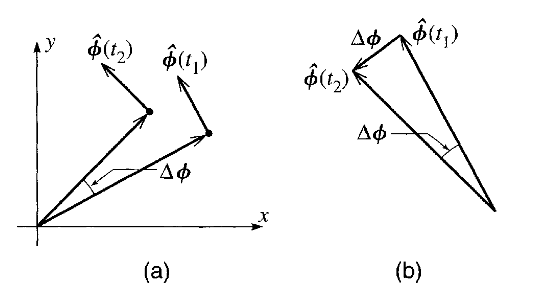
\includegraphics[width=0.65\linewidth]{polarDerivatives2.png}
    \caption{\bf{(a)} $\Delta \phihat$ is solely dependent on $\Delta\phi$. \bf{(b)} $\Delta\phihat$ is determined by the pictured triangle.}
    \label{fig:polarDerivatives2}
\end{figure}

We can use the law of cosines once again to see
\[ \abs{\Delta\phihat} = \sqrt{2-2\cos\Delta\phi} \]
which, using the same approximation as (\ref{small_angle_polar_unit}), we once find $\abs{\Delta \phihat} \approx \Delta \phi$. By placing the tip of $\phihat(t_1)$ at the tip of $\phihat(t_2)$, we can subtract them geometrically and convince ourselves that $\Delta \phihat$ points in the direction $-\rhat$. Thus, we obtain
\[ \Delta\phihat \approx -\Delta \phi \rhat(t_1)\]
or
\[ \frac{\Delta \phihat}{\Delta t} \approx -\frac{\Delta \phi}{\Delta t}\rhat(t_1)\]
once again taking the limit as $\Delta t\to 0$, we get
\[ \dotunit{\phi} = -\dot \phi \rhat\]
Substituting this and $\dotunit{r} = \dot{\phi}\phihat$ into (\ref{polar_a_unsimplified}), we find
\begin{equation} \label{polaracceleration}
    \mbf{a} = \pqty{\ddot r - r\dot{\phi}^2}\rhat + \pqty{2\dot{r}\dot\phi + r\ddot{\phi}}\phihat
\end{equation}
This result in its full generality is quite difficult to interpret, so we will consider the special case where $r$ is fixed. This means that $\dot r = \ddot r = 0$, so
\[ \mbf{a} = -r\dot{\phi}^2\rhat + r\ddot{\phi}\phihat \]
or
\[ \mbf{a} = -r\omega^2\rhat + r\alpha \phihat\]
where $\omega = \dot r$ is defined as before and $\alpha = \ddot r$ is the angular acceleration. This describes the common result from elementary physics that an object moving in circular motion with a fixed radius has an inward radial ``centripetal" acceleration given by $r\omega^2 = v^2/r$ and a tangential acceleration $r\alpha$.

With (\ref{polaracceleration}), we can now write down Newton's Second Law in polar form:
\[ \mbf F = m\mbf{a} = (m\ddot r - mr\dot{\phi}^2)\rhat + (mr\ddot \phi + 2\dot{r}\dot{\phi})\phihat\]
\begin{example}[An Oscillating Skateboard]
    A smooth half-pipe at a skate park consists of a concrete trough with a semicircular cross section of radius $R$. A skateboard is released from rest at an angle $\phi=\phi_0$ from the vertical. Determine an expression for the movement of the skateboard as $t$ varies, and determine when the skateboard returns to its original position.   
    
    \begin{minipage}{0.48\textwidth}
        This is a problem where polar coordinates will prove extremely useful. We will define the origin $O$ aligned vertically with the top of the half-pipe and aligned horizontally with the middle of it, as shown in the figure to the right. We will also define $\phi=0$ to be the line pointing straight down, with counterclockwise being the direction of increasing $\phi$.
    \end{minipage}
    \begin{minipage}{0.48\textwidth}
        \parbox{\textwidth}{
            \label{half-pipe}
            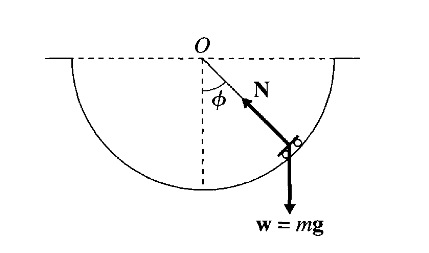
\includegraphics[width=\textwidth]{halfPipe.png}
        }
    \end{minipage}
    
    Because the radius is held constant at $r=R$, Newton's Second law tells us 
    \[ \mbf{F} = -mR\dot{\phi}^2\rhat + mR\ddot{\phi}\phihat \]
    The two forces on the skateboard are the weight force $\mbf{w}$ and the normal force $\mbf{N}$. $\mbf{N}$ acts solely in the $-\rhat$ direction. With some trigonometry, we can determine that $\mbf{w} = mg\cos\phi\rhat - mg\sin\phi\phihat$. Thus the motion of the skateboard is determined by the equations
    \[ -mR\dot{\phi}^2 = mg\cos\phi - N \quad \text{and} \quad mR\ddot{\phi} = -mg\sin\phi\]
    We aren't particularly interested in the left equation, as we are able to fully solve for the motion with just the one on the right. We can rearrange to obtain
    \[ \ddot\phi = -\frac{g}{R}\sin\phi \]
    which is a second order differential equation for $\phi$. Due to the nonlinearity of this equation, it is impossible to solve in terms of elementary functions. Instead, we will make the approximation $\sin\phi\approx\phi$ to find 
    \[ \ddot\phi = -\frac{g}{R}\phi \]
    We will define a quantity $\omega = \sqrt{g/R}$ as the \textit{angular frequency} of the oscillation, and then the general solution is given by
    \[ \phi(t) = A\sin(\omega t) + B\cos(\omega t)\]
    With the initial condition $\phi(0) = \phi_0$ and $\phi'(0)=0$, obtain a particular solution given by
    \[ \phi(t) = \phi_0\cos(\omega t)\]
    To determine how long it will take for the skateboard to return to its original position, we will rely on the periodicity of the cosine function. If $\phi_0\cos(\omega t) = \phi_0$, then we must have $\omega t = 2\pi n$ for some natural number $n$. The earliest such time besides $t=0$ is given by choosing $n=1$, so $t = 2\pi/\omega$. 

    We call this time the \textit{period} of the oscillation, and denote it with $\tau$.

    \begin{minipage}{0.48\textwidth}
    While the approximation $\sin\phi\approx\phi$ is remarkably effective for relatively small $\phi$, it is important to note that it is only an approximation. If we have a large initial condition, such as $\phi_0 = \pi/3$, the small angle approximation is no longer accurate and will lead to significant deviation between the approximated solution and the real solution. For an example of this, see the figure on the right, which plots $\phi$ versus $t$ for $R=5$ and $\phi_0 = \pi/3$. Clearly, there is significant error between the approximated solution (blue), and the true solution (red), which was obtained via numerical methods.
    \end{minipage}
    \begin{minipage}{0.48\textwidth}
        \parbox{\textwidth}{
            \label{error}
            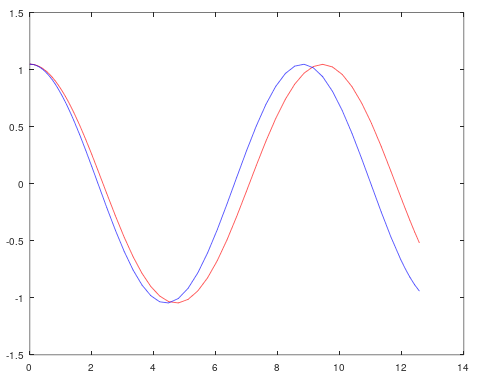
\includegraphics[width=\textwidth]{approximationError.png}
        }
    \end{minipage}
\end{example}
 % newton's laws
\chapter{Particles and Charged Particles}
\section{Air Resistance} \label{drag1}
We often ignore the air resistance of objects moving through the air in introductory physics. While this is often a good approximations, there are certainly cases where air resistance has a non-negligible effect on the path of the object, and should not be ignored.

Most of what we go over in this section is applicable to just about any fluid--the mechanics of air resistance is modeled by the same equations as the drag of a general fluid. 

Throughout this section, we will make the assumption that the direction of the drag force $\mbf{f}$ acts in the opposite direction as the velocity $\mbf{v}$ of the object. This is an approximation and indeed has cases where it fails to describe the behavior of objects. For instance, the drag on an airplane wing has a component pointing upwards (the force of \textit{lift}), and no planes would be able to fly without it. A more complete exploration of drag is more suited for a fluid dynamics text, so we will continue with our approximation.

The drag force, in our approximation, will be solely dependent on the speed $v$ of the object, so it can be written as
\[ \mbf{f} = -f(v)\mbf{\hat v} \]
From elementary calculus, we know that we can write $f(v)$ as a Taylor Series
\[ f(v) = a + bv + cv^2 + \cdots \]
Because $f(v) = 0$ when $v=0$ (otherwise objects would have air resistance even without moving), we know that $a_0 = 0$. We will also approximate $f$ with just the $v$ and $v^2$ terms, as they are more than enough for more practical purposes. 

Therefore our model for drag is 
\[ \mbf{f} = (bv + cv^2)\mbf{\hat v}\]
we will split the drag into a linear and quadratic component $f_{\text{lin}} = bv$ and $f_{\text{quad}} = cv^2$. Through experimental methods, it has been determined that the quadratic term primarily arises from the object having to accelerate the air it hits, and is proportional to the surface area of the projectile. The linear term primarily arises from the viscous drag of the medium, which is proportional to the linear size of the projectile. 

Therefore, if we approximate our object as a sphere of diameter $D$, we can write
\[ f(v) = bv + cv^2 = \beta Dv + \gamma D^2v^2 \]
The values of $\beta$ and $\gamma$ are constant, and have been determined to be equal to approximately 
\[ \beta = 1.6\times 10^{-4}\,\si{\newton\second\per{\meter\tothe{2}}} \]
and
\[ \gamma = 0.25 \, \si{\newton\square\second\per\meter{\tothe{4}}} \]
when measured for a spherical projectile in air at STP. Oftentimes, the drag force will be largely dominated by either the quadratic term or the linear term, and so the other can be ignored. To determine when this is the case, consider the ratio $f_{\text{quad}}/f_{\text{lin}}$. This is given by
\begin{equation} \label{quadlinearratio}
    \frac{f_{\text{quad}}}{f_{\text{lin}}} = \frac{\gamma D^2v^2}{\beta Dv} = \pqty{1.6\times10^3 \,\si{\second\per\square\meter}}Dv
\end{equation}
\begin{example}
    Assess the relative importance of the linear and quadratic terms for a baseball of diameter $D_1 = 7\,\si{\centi\meter}$ traveling at a speed of $v_1 = 5\,\si{\meter\per\second}$. Repeat this for a raindrop with diameter $D_2 = 1\,\si{\milli\meter}$ and speed $v_2 = 0.6\,\si{\meter\per\second}$ and for a droplet of oil with diameter $D_3 = 1.5\,\si{\micro\meter}$ and speed $v_3 = 5\times10^{-5}\,\si{\meter\per\second}$.

    First we will convert both diameters into meters to obtain $D_1 = 7\times10^{-2}\,\si{\meter}$, $D_2 = 10^{-3}\,\si{\meter}$, and $D_3 = 1.5\times10^{-6}\,\si{\meter}$. Then, we simply plug the numbers into (\ref{quadlinearratio}) for each object.

    For the baseball, we get
    \[ \frac{f_{\text{quad}}}{f_{\text{lin}}} \approx 600 \]
    This means that the term for quadratic drag is roughly 600 times greater than the term for linear drag, so we can safely ignore it. 

    For the raindrop,
    \[ \frac{f_{\text{quad}}}{f_{\text{lin}}} \approx 1\]
    This means that the quadratic and linear term are comparable in size, and so neither can be safely ignored.

    Finally, for the oil drop,
    \[ \frac{f_{\text{quad}}}{f_{\text{lin}}} \approx 10^{-7} \]
    So the quadratic term is totally negligible and we can focus solely on linear drag.
\end{example}
Another method of examining the relative importance of linear and quadratic drag is known as the \textit{Reynolds number}, and is a dimensionless quantity defined with $R = Dv\rho/\eta$, where $D$ and $v$ are defined as expected, $\rho$ is the density of the fluid, and $\eta$ is the viscosity of the fluid. $R$ will end up being about the same order of magnitude as the ratio $f_{\text{quad}}/f_{\text{lin}}$. Thus when $R$ is large the quadratic force dominates and when $R$ is small the linear force dominates.
\section{Linear Air Resistance}
Consider a particle for which the quadratic drag force is negligible and the only two forces acting on it are the gravitational force and linear drag. Its initial velocity is given by $\mbf{v}(t_0) = \mbf{v_0}$ and its initial position is the origin. The equation of motion of this particle is given by
\[ m\mbf{\ddot r} = mg\mathbf{\hat\jmath} - b\mbf{\dot r} \]
where $\hat{\jmath}$ is defined as pointing towards the surface of the earth. This is a second order differential equation for $\mbf{r}$, but we are actually able to reduce it into a first order differential equation for $\mbf{\dot r} = \mbf{v}$ by writing $\mbf{\ddot r} = \mbf{\dot v}$, so
\[ m\mbf{\dot v} = mg\yhat - b\mbf{v} \]
Breaking this into its components, we get the uncoupled system 
\begin{align*}
    m\dot v_y &= mg - bv_y \\
    m\dot v_x &= -bv_x 
\end{align*}
this system is quite easy to solve because it can be thought of as two separate first order equations for $v_x$ and $v_y$. We will begin with $v_x$ because it is easier to solve than $v_y$. 
\subsection*{Horizontal Motion with Linear Drag}
First, rearrange the differential equation to obtain
\[ \dot v_x = -\frac{b}{m}v_x\]
This is a separable differential equation with solution
\[ v_x(t) = v_{x0}e^{-bt/m}\]
We will define the quantity $\tau = m/b$ as the \textit{time constant}, so
\[ v_x(t) = v_{x0}e^{-t/\tau} \]
The time constant can be interpreted as the amount of time it takes for the velocity to decrease by a factor of $1/e$. For instance,
\[ v_x(\tau) = v_{x0}e^{-\tau/\tau} = v_{x0}e^{-1} \]
and
\[ v_x(2\tau) = v_{x0}e^{-2} = e^{-1}v_x(\tau)\]
As $t\to\infty$, the $x$-velocity approaches zero, and the position converges to a finite number. To see this, we calculate $x(t)$ as
\begin{align*}
    x(t) &= x(0) + \int_0^t v_x(t')\dd t' \\
    &= 0+ \bqty{-v_{x0}\tau e^{-t'/\tau}}_0^t \\
    &= v_{x0}\tau(1-e^{-t/\tau})
\end{align*}
Noting that $\lim\limits_{t\to\infty} x(t) = v_{x0}\tau$, we define a parameter $x_{\infty}\equiv \tau v_{x0}$, so
\[ x(t) = x_{\infty}(1-e^{-t/\tau})\]
$x(t)$ will therefore asymptotically approach $x_{\infty}$ as time goes on.
\subsection*{Vertical Motion with Linear Drag}
Now we draw our attention to the $y$ direction. Recall the differential equation
\[ m\dot v_y = mg - bv_y\]
Before we attempt to actually solve the equation, we can reason that $v_y$ will eventually reach some \textit{terminal velocity} when the force on it is zero, or when
\[ v_{\text{ter}} \equiv v_y = \frac{mg}{b} \]
The differential equation for $v_y$ is a first order linear equation, and can be solved with the method of integrating factors. First rewrite to obtain
\[ \dot v_y + \frac{b}{m}v_y = g \]
or
\[ \dot v_y + \frac{1}{\tau}v_y = g\]
and then apply the integrating factor with $\mu(t) = \exp\pqty{t/\tau}$, so
\begin{align*}
    \dv{t}\pqty{e^{t/\tau}v_y(t)} &= ge^{t/\tau} \\
    e^{t/\tau}v_y(t) &= \frac{mg}{b}e^{t/\tau} + C \\
    v_y(t) &= v_{\text{ter}} + Ce^{-t/\tau}
\end{align*}
With the initial condition $v_y(0)= v_{0y}$, we get $C = v_{0y}-v_{\text{ter}}$, so
\[ v_y(t) = v_{0y}e^{-t/\tau} + v_{\text{ter}}(1 - e^{-t/\tau}) \]
Because $v_y$ approaches a nonzero number as $t\to\infty$, $y(t)$ will diverge. But we can still find an expression for it at a finite $t$ by integrating.
\begin{align*}
    y(t) &= y(0) + \int_0^tv_{0y}e^{-t'/\tau} + v_{\text{ter}}(1 - e^{-t'/\tau})\dd t' \\
    &= v_{\text{ter}}t + \tau(v_{0y}-v_{\text{ter}})(1-e^{-t/\tau})
\end{align*}
Thus the full equations of motion for our system have been found
\[ \pmat{x(t) \\ y(t)} = \pmat{ v_{x0}\tau (1-e^{-t/\tau}) \\ v_{\text{ter}}t + \tau(v_{0y}-v_{\text{ter}})(1-e^{-t/\tau})}\]
\subsection*{Range and Trajectory of Movement with Linear Drag}
For this section, it will be marginally more convenient to swap the sign of $\yhat$, so it points upwards. The new equations of motion are given by
\[ \pmat{x(t) \\ y(t)} = \pmat{ v_{x0}\tau (1-e^{-t/\tau}) \\  \tau(v_{0y}+v_{\text{ter}})(1-e^{-t/\tau}) - v_{\text{ter}}t}\]
To analyze the range of the projectile, we first need to get $y$ as a function of $x$. Using standard methods, we can eliminate $t$ and obtain
\begin{equation} \label{yofx_airres}
     y = \frac{v_{y0} + v_{\text{ter}}}{v_{x0}}x + v_{\text{ter}}\tau\ln\pqty{1 - \frac{x}{v_{x0}\tau}}
\end{equation}
This equation is probably too complex to bring any real value, so we will instead graph it to get an idea for what it represents.
\begin{figure}[h!]
    \centering
    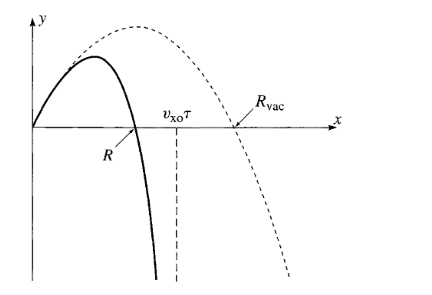
\includegraphics[width=0.5\linewidth]{rangeLinearDrag.png}
\end{figure}

Where the solid line is the trajectory with air resistance and the dotted line is the trajectory without. We can make a few observations about this graph.
\begin{enumerate}
    \item The graph passes the $x$ axis (i.e. $y=0$) twice--first when $x=0$ and second at some nonzero $x=R$. This value $R$ represents the range of the projectile, assuming the ground is level. 
    \item The graph approaches a vertical asymptote as $x\to v_{x0}t$, with $y$ diverging to $-\infty$. This happens because $x$ is approaching its steady state $x_\infty = v_{x0}\tau$, but $y$ is still decreasing without bound.
    \item The graph initially matches the trajectory of the projectile in a vacuum, but resembles it less and less as $x$ increases.
\end{enumerate}
In elementary physics we found the range of a particle launched at an initial $y$ speed $v_{y0}$ and x speed $v_{x0}$ above a level horizontal ground to be
\[ R_{\text{vac}} = \frac{2v_{x0}v_{y0}}{g}\]
Where $R_{\text{vac}}$ stands for the range in a vacuum. By introducing air resistance, we obtain an implicit definition of $R$ by setting (\ref{yofx_airres}) equal to zero:
\begin{equation} \label{rangelevelres}
    \frac{v_{y0} + v_{\text{ter}}}{v_{x0}}R + v_{\text{ter}}\tau\ln\pqty{1 - \frac{R}{v_{x0}\tau}} = 0
\end{equation}
if the ground was not level and instead decreased in height by some $h$, the equation would instead be
\[ \frac{v_{y0} + v_{\text{ter}}}{v_{x0}}R + v_{\text{ter}}\tau\ln\pqty{1 - \frac{R}{v_{x0}\tau}} = -h\]
In fact, if the height of the ground was modeled by \textit{any} function $h(x)$, we could find the point where the projectile hits the ground by finding the solution to
\[ \frac{v_{y0} + v_{\text{ter}}}{v_{x0}}R + v_{\text{ter}}\tau\ln\pqty{1 - \frac{R}{v_{x0}\tau}} = h(R) \]
None of these equations can be solved analytically, so we must instead employ numerical methods or approximations. 
% Returning our focus to the case where the ground is level, we can find an approximate solution by noting that
% \[ \ln(1-\epsilon) = -\pqty{\epsilon + \frac{1}{2}\epsilon^2 + \frac{1}{3}\epsilon^3 + \cdots }\]
% and for small values of epsilon (which occur when $x$ is relatively small compared to $v_{x0}\tau$), 
% \[ \ln(1-\epsilon) \approx -\pqty{\epsilon + \frac{1}{2}\epsilon^2 + \frac{1}{3}\epsilon^3}\]
% plugging this approximation into \ref{rangelevelres}, we find
% \[ \pqty{\frac{v_{y0}}{v_{x0}}R + \frac{v_{\text{ter}}}{v_{x0}}R} - v_{\text{ter}}\tau\pqty{\frac{R}{v_{x0}\tau} + \frac{1}{2}\pqty{\frac{R}{v_{x0}\tau}}^2 + \frac{1}{3}\pqty{\frac{R}{v_{x0}\tau}}^3} = 0\]
% Noting that the second term in the left bracket cancels with the first term in the right bracket, we get
% \[ -R\pqty{-\frac{v_{y0}}{v_{x0}} + \frac{v_{\text{ter}}}{2v_{x0}^2}\pqty{\frac{R}{\tau}} + \frac{v_{\text{ter}}}{3v_{x0}^3}\pqty{\frac{R}{\tau}}^2} = 0\]
% This gives two solutions: first, there's of course $R=0$. Then, there is the solution to
% \[ -\frac{v_{y0}}{v_{x0}} + \frac{v_{\text{ter}}}{2v_{x0}^2}\pqty{\frac{R}{\tau}} + \frac{v_{\text{ter}}}{3v_{x0}^3}\pqty{\frac{R}{\tau}}^2 = 0\]
% Some rearrangement of this equation gives
% \begin{equation} \label{quadrefr}
%     R = \frac{2v_{y0}v_{x0}}{g}-\frac{2}{3v_{x0}\tau}R^2
% \end{equation}
% where I replaced $v_{\text{ter}}/{\tau}$ with $g$. This may seem like an odd way to phrase the quadratic equation, but it ends up being quite insightful. 

% In general, when the effect of air resistance is small, $\tau$ gets very large, causing the right term in (\ref{quadrefr}) to get small. Therefore, for small air resistance,
% \[ R \approx \frac{2v_{y0}v_{x0}}{g} = R_{\text{vac}} \]
% If air resistance is still small but not entirely negligible, we can replace the $R$ on the right side of (\ref{quadrefr}) with $R_{\text{vac}}$ while keeping the $R$ on the left side, giving
% \begin{align*}
%     R &\approx R_{\text{vac}}-\frac{2}{3v_{x0}\tau}R_{\text{vac}}^2 \\
%     &= R_{\text{vac}}\pqty{1-\frac{4}{3}\frac{v_{y0}}{v_{\text{ter}}}}
% \end{align*}
% Note that the second $R_{\text{vac}}$ in the rightmost term was replaced with $2v_{y0}v_{x0}/g$.

\section{Quadratic Air Resistance}
We were able to develop a rather complete theory of the behavior of projectiles subject to a linear drag force. While some projectiles do follow the rules of linear drag quite accurately (such as the oil drop we explored as an example in Section \ref{drag1}), most larger projectiles will be more accurately modeled by quadratic drag. Unfortunately, the theory of quadratic drag is far less developed than its linear counterpart, and finding an analytical solution to
\[ m\mbf{\dot v} = mg\yhat - bv^2\mbf{\hat v} \]
in terms will prove to be impossible when there is movement in both the $\yhat$ and $\xhat$ directions. The reason that $m\mbf{\dot v} = mg\yhat - b\mbf{v}$ was so much easier to solve than the quadratic counterpart is that it is a \textit{linear differential equation}, for which there is a quite comprehensive and relatively simple theory. In fact, some nonlinear equation will give rise to the phenomenon known as chaos. 
\subsection*{Horizontal Motion with Quadratic Drag}
Although we cannot explicitly solve for the motion of objects moving freely in two dimensions, we are able to solve for objects constrained to move along a single axis.

Consider an object moving horizontally in the $\xhat$ direction, with no net force in the $\yhat$ direction. The force can then be written as
\[ m\dot v = -cv^2 \]
Note that we do not include the subscript $x$ because this is a one-dimensional problem, so it is unnecessary.

this is quite simple to solve via the method of separation of variables:
\[ m\int_{v_0}^{v} \frac{d\nu }{\nu^2} = -c\int_0^t \dd t'\]
where $v(0) = v_0$. Integrating both sides, we obtain
\[ m\pqty{\frac{1}{v_0} - \frac{1}{v}} = -ct \]
which simplifies to
\[ v(t) = \frac{1}{1/v_0 + ct/m} = \frac{v_0}{1+cv_0t/m}\]
Denoting $m/(cv_0) \equiv \tau$ as the time constant for quadratic drag, we get
\[ v(t) = \frac{v_0}{1+t/\tau} \]
Then, to get the position $x(t)$, we simply have to integrate $v(t)$ to obtain
\begin{align*}
    x(t) &= x(0) + \int_0^t \frac{v_0}{1+t'/\tau}\dd t' \\
    &= x_0 + v_0\tau \ln(1 + t/\tau) 
\end{align*}
Critically, unlike the case of linear drag, $x$ will increase without bound when subject to quadratic drag. The velocity will go to zero regardless of whether the drag is linear or quadratic. When the drag is linear, however, the velocity will decrease exponentially, whereas quadratic drag only causes the velocity to decrease on the order of $1/t$ (much slower than an exponential decrease). This seems to suggest that it is unrealistic for an object to experience a primarily quadratic drag force at \textit{all times}. As the speed goes down, the linear term will begin to become increasingly significant. This can be seen by the fact that the Reynold's number decreases linearly as $v$ decreases.
\subsection*{Vertical Motion with Quadratic Drag}
In the case where an object moves linearly with a quadratic drag force, we will solve it through similar methods as the horizontal case. Consider an object dropped off a roof. The equation of motion is given by
\[ m\dot v = mg - cv^2 \]
where the positive direction is towards the ground. We can clearly see that there is a steady state at
\[ v_{\text{ter}} = \sqrt{\frac{mg}{c}} \]
We can tidy up the equation of motion slightly to find
\[ \dot v = g\pqty{1 - \frac{v^2}{v_{\text{ter}}^2}}\]
This can be solved with the method of separation of variables:
\begin{align*}
    \int_{0}^v \frac{1}{1-v^2/v_\text{ter}^2}\dd v &= \int_0^t g\dd t' \\
    v_\text{ter}\pfn{arctanh}\pqty{\frac{v}{v_\text{ter}}} &= gt
\end{align*}
Which can be solved for $v$ to obtain 
\[ v(t) = v_\text{ter}\tanh\pqty{\frac{g}{v_\text{ter}}t}\]
and then integrated to obtain an expression for $y$:
\[ y(t) = \frac{v_\text{ter}^2}{g}\ln\bqty{\cosh\pqty{\frac{gt}{v_\text{ter}}}}\]
\subsection*{Quadratic Drag with Horizontal and Vertical Motion}
As said previously, it is not possible to find a general expression for the position of an object subject to quadratic drag in multiple directions simultaneously. Numerical methods, however, are still on the table.

The equations of motion governing an object subject to quadratic drag and gravity are given by
\[ m\mbf{\ddot r} = mg\yhat - cv^2\mbf{\hat v}\]
or
\[ m\mbf{\ddot r} = mg\yhat - cv\mbf{v}\]
component-wise, this turns into
\begin{align*}
    m\dot v_x &= -cv_x\sqrt{v_x^2+v_y^2} \\
    m\dot v_y &= mg - cv_y\sqrt{x_x^2+v_y^2} 
\end{align*}
There is no way to solve these coupled equations, but software such as MATLAB, Mathematica, or python are fully capable of giving highly accurate graphs for a given initial condition via numerical methods.
\section{Motion of a Charge in a Uniform Magnetic Field}
Another interesting application of Newton's laws is the motion of a charged particle within a magnetic field. Consider a positive charge $q$ moving in a uniform magnetic field $\mbf{B}$ that points in the $\zhat$ direction. The net force on the particle is just the magnetic force
\[ \mbf{F} = q\mbf{v}\times\mbf{B} \]
So the equation of motion of the particle is
\[ m\mbf{\dot v} = q\mbf{v}\times\mbf{B} \]
We will split this problem into components to attempt to solve it. Suppose $\mbf{v} = (v_x, v_y, v_z)$ and $\mbf{B} = (0,0,B)$. Then,
\[ \mbf{v}\times\mbf{B} = \vmat{\xhat & \yhat & \zhat \\ v_x & v_y & v_z \\ 0 & 0 & B } = (v_yB, -v_xB, 0) \]
Therefore the equation of motion of the system is
\[ \pmat{m\dot v_x \\ m\dot v_y \\ m\dot v_z} = \pmat{qv_yB \\ -qv_xB \\ 0 }\]
The third component just tells us that $v_z$ is simply constant, so we will focus our attention solely on $v_x$ and $v_y$. We can define a new vector consisting of only the projection of $\mbf{v}$ onto the $xy$-plane. In other words, $v_T = (v_x, v_y)$. This is known as the \textbf{transverse velocity}.

We will also define the parameter $\omega = qB/m$ as the \textbf{cyclotron frequency}. With this notation, we get the coupled system of two differential equations
\begin{align*}
    \dot v_x &= \omega v_y \\
    \dot v_y &= -\omega v_x 
\end{align*}
It may be immediately clear from observation that $v_x$ and $v_y$ will consist of sinusoidal functions, but we will explore a different way to solve for them involving complex numbers. This isn't necessarily the easiest solution for the current problem, but an introduction to the mathematical methods used in it will prove valuable.

Define a complex number $\eta\in\C$ as
\[ \eta = v_x + iv_y \]
The real part of $\eta$ can be thought of as representing an $x$ coordinate in the complex plane, and the imaginary part of $\eta$ can be thought of as representing a $y$ coordinate. Therefore $\eta$ is analogous to the transverse velocity vector. The advantage of this representation is that by differentiating $\eta$, we find
\begin{align*}
    \dot \eta &= \dot v_x + i \dot v_y = \omega v_y - i \omega v_x \\
    &= -i\omega(v_x + iv_y) = -i\omega\eta 
\end{align*}
The differential equation $\dot\eta = -i\omega\eta$ is extremely familiar, and we know it to have the solution $\eta = Ae^{-i\omega t}$ where $A\in\C$. Then, we can find the components of position by writing $\xi = x + iy$. We have the relationship $\dot\xi = \eta$, so
\[ \xi = \int \eta \dd t = \frac{Ai}{\omega}e^{-i\omega t} + Z\]
defining $Ai/\omega = C$ and $Z = X+iY$, we find
\[ x + iy = Ce^{-i\omega t} + (X + iY) \]
if we define our origin such that the central position $(X,Y)$ is $(0,0)$, we obtain
\[ x + iy = Ce^{-i\omega t} = (x_0 + iy_0)e^{-i\omega t} \]
This describes a circle in the $xy$ plane with initial position $(x_0, y_0)$ that rotates clockwise with an angular frequency $\omega$. Recalling that $\dot v_z = 0$, we get $z(t) = z_0 + v_zt$, so the overall position vector is described by
\[ \pmat{x\\y\\z} = \pmat{\Re{(x_0+iy_0)e^{-i\omega t}} \\ \Im{(x_0+iy_0)e^{-i\omega t}} \\ z_0 + v_zt}\]
If desired, the expression $(x_0+iy_0)e^{-i\omega t}$ can be fully split into its real and imaginary components by applying Euler's formula. This, however, isn't necessary here as we already understand the physical interpretation of the real and imaginary parts of $x+iy$, so it would just be an algebraic nightmare that gives no real insight.  % projectiles and charged particles
\chapter{Momentum and Angular Momentum}
\section{Conservation of Momentum}
Previously we stated the law of conservation of momentum, which states that for a system of $N$ particles, the rate of change of linear momentum on the system $\mbf{P} = \sum_\alpha \mbf{p}_\alpha$ is determined by the net external force on the system
\[ \mbf{\dot P} = \mbf{F}^{\text{ext}} \]
so if the net external force is zero, the total momentum is constant. This principle can help us solve many problems, such as the one below.
\begin{example}
    Two bodies have masses $m_1$ and $m_2$ and are travelling at velocities $\mbf{v}_1$ and $\mbf{v}_2$ before colliding with each other and sticking together, moving with some final velocity $\mbf{v}_\text{fin}$. Find $\mbf{v}_\text{fin}$. 

    The principle of conservation of momentum tells us that the total momentum on the system is the same before and after the collision, since there are no external forces. The momentum just before the collision is
    \[ \mbf{P}_{\text{in}} = m_1\mbf v_1 + m_2\mbf v_2 \]
    and the momentum just after is
    \[ \mbf{P}_{\text{fin}} = m_1\mbf v_\text{fin} + m_2\mbf v_\text{fin} = (m_1 + m_2)\mbf{v}_\text{fin}\]
    Equating these two, we have
    \[ (m_1+m_2)\mbf{v}_\text{fin} = m_1\mbf v_1 + m_2\mbf v_2 \]
    and then dividing by $m_1+m_2$,
    \[ \mbf{v}_\text{fin} = \frac{m_1\mbf v_1 + m_2\mbf v_2}{m_1+m_2}\]
\end{example}
\section{Rockets}
One large application of the principle of conservation of momentum is in the physics behind rockets. The basic question a rocket must answer is this: With no external agent to push you, how do you accelerate yourself? 

To answer this question, imagine you are trapped in the middle of a completely frictionless frozen lake. It is impossible to accelerate yourself by walking, as there is no friction to let you move. The simplest way to accelerate yourself is to throw something with a lot of mass in the opposite direction you want to go. As you throw the object, the reaction force from you throwing it pushes you backwards.

Rockets make use of this idea to its extreme. The rocket's motor hurls fuel into the air behind it, which pushes the rocket forward.

To analyze this situation mathematically, consider a rocket with mass $m$, traveling in the positive $\xhat$ direction and ejecting fuel with a velocity $v_\text{ex}$ relative to the rocket. At a time $t$, the rocket's momentum is $P(t) = mv$. At time $t + \dd t$, the mass of the rocket is $m + \dd m$, where $\dd m$ is negative, and its momentum is $(m + \dd m)(v + \dd v)$. The fuel ejected in that time $\dd t$ has mass $-\dd m$ and a velocity of $v - v_\text{ex}$ relative to the ground. 

Thus the total momentum of the rocket-fuel system at $t+\dd t$ is
\begin{align*}
    P(t + \dd t) &= (m+\dd m)(v+\dd v) - \dd m(v - v_\text{ex}) \\
    &= mv + v\dd m + m \dd v + \dd m \dd v - v\dd m + v_\text{ex}\dd m  \\
    &\approx mv + m \dd v + v_\text{ex}\dd m 
\end{align*}
where the $\dd m \dd v$ term is disregarded because of its tiny size, as the product of two differentials. 

The change in momentum is $\dd P = P(t + \dd t) - P(t) = m\dd v + v_\text{ex}\dd m$. If there is some external force $F^\text{ext}$ (gravity, for instance), then $\dd P = F^\text{ext}$. Here, we will assume there is no external force, so $\dd P = 0$. This allows us to write
\[ m \dd v = -v_\text{ex}\dd m \]
or
\begin{equation} \label{thrust}
     m \dot v = -v_\text{ex}\dot m 
\end{equation}
Where $\dot m$ is the rate at which the rocket's engine is ejecting mass. This equation is essentially the equivalent of Newton's Second Law for rockets, where $-v_\text{ex}\dot m$ plays the role of the force. For this reason, we refer to the quantity $-v_\text{ex}\dot m$ as the \textbf{thrust} of the rocket. 

Because $\dot m$ is negative, the thrust is a positive quantity. 

(\ref{thrust}) is a separable differential equation and can be solved quite easily:
\begin{align*}
    \int_{v_0}^v\dd v &= -v_\text{ex} \int_{m_0}^m \frac{\dd m}{m} \\
    v - v_0 &= v_\text{ex}\ln(m_0/m)
\end{align*}
This result puts a significant restriction on the speed of the rocket. The increase in speed is determined by the size of the term $\ln(m_0/m)$, which is at its maximum when all fuel is burned and the remaining mass is just the rocket itself and the payload. 

Even if $90\%$ of the rocket's mass is fuel that was burned, $\ln(m_0/m)$ is still only equal to about $2.3$, and the velocity cannot be more than $2.3$ times bigger than $v_\text{ex}$. To combat this, rocket engineers spend a significant amount of time trying to maximize $v_\text{ex}$ and reduce the final mass (this is why rockets often detach from their fuel tanks after emptying them). 

\section{Center of Mass}
Consider a group of $N$ particles with masses $m_i$ and positions $\mbf{r}_i$ measured relative to some origin $O$. The \textbf{center of mass} of this system is defined as the position relative to $O$ given by
\[ \mbf R = \frac{\sum m_i\mbf{r}_i}{\sum m_i}\]
by writing the total mass of the system as $M = \sum m_i$, then $\mbf R = \frac{1}{M}\sum m_i\mbf{r}_i$. This equation can be quite easily split into three equations, one for each component.

Another way to think about the center of mass $\mbf{R}$ is as a weighted average of all the individual positions, with each $\mbf{r}_i$ having a weight of $m_i$. 

In the case where there are only two masses, the center of mass is
\[ \mbf{R} = \frac{m_1\mbf{r}_1 + m_2\mbf{r}_2}{m_1+m_2} \]
From this definition, it is pretty simple to show that the center of mass of $m_1$ and $m_2$ lies on the line joining $\mbf{r}_1$ and $\mbf{r}_2$, and the ratio of the distances between ($\mbf{R}$ and $\mbf{r_1}$) and ($\mbf{R}$ and $\mbf{r}_2$) is equal to $m_1/m_2$. 

If $m_1$ is much greater than $m_2$, then $\mbf{R} \approx \mbf{r}_1$, and vice versa if $m_2$ is much greater than $m_1$. This also extends to the $N$-particle case--if $m_1$ is much greater than all of the other masses, then $\mbf{R}\approx \mbf{r}_1$. An example of this is our solar system. The sun is much more massive than every other planet (and all of the non-planet objects as well), so the center of mass of the solar system is approximately equal to the position of the sun. 

We are also able to write
\[ M\mbf{R} = \sum m_i\mbf{r}_i\]
And then differentiate to find
\[ M\mbf{\dot R} = \sum m_i \mbf{\dot r}_i \]
But $\sum m_i\mbf{\dot r}_i$ is just the total momentum of the system. Therefore,
\[ \mbf{P} = M\mbf{\dot R} \]
We can differentiate once again and use $\mbf{F}^\text{ext} = \mbf{\dot P}$ to write
\[ \mbf{F}^\text{ext} = M\mbf{\ddot R}\]
This shows an extremely crucial result that allows us to generalize many of our results from studying particles to actual scenarios--the center of mass of a system of particles moves exactly as if it were a single particle of mass $M$.

The concept of the center of mass can be extended to continuous distributions of mass using integration. For some three-dimensional volume $V$ with a mass distribution $\rho(x,y,z)$, then
\[ \mbf{R} = \frac{1}{M} \iiint\limits_V \rho \, \mbf{r}\, \dd V \]
where $M = \iiint\limits_V \rho \, \dd V$ is the mass of $V$. The same concepts apply to one-dimensional or two-dimensional mass distributions.
\begin{example}[Center of Mass of a Solid Cone]
    A cone with a constant density $\rho$ has a radius of $R$ and a height $h$. Find its center of mass. 

    It makes the most sense to analyze this problem through cylindrical coordinates. We will orient our cone so that its vertex is at the origin $O$, and it gets wider as the $z$ coordinate increases. At each height $z$, the horizontal cross section is a circle of radius $r = Rz/h$. We can rearrange this to $z = hr/R$, and set up our triple integral as 
    \begin{align*}
        \mbf R = \frac{1}{M} \iiint\limits_V \rho \mbf r \dd V &= \frac{1}{M} \int_0^{2\pi}\int_0^{R}\int_{hr/R}^h \rho r \mbf r \dd z \dd r \dd \theta
    \end{align*}
    But before we evaluate this, we should first find the mass $m$.
    \begin{align*}
        M = \iiint\limits_V \rho \dd V &= \int_0^{2\pi}\int_0^R\int_{hr/R}^h \rho r\dd z\dd r\dd \theta \\
        &= 2\pi\rho \int_0^R \pqty{rh - \frac{r^2h}{R}}\dd r \\
        &= 2\pi\rho \pqty{\frac{R^2h}{2} - \frac{R^2h}{3}} = \frac{1}{3}\rho \pi R2 h 
    \end{align*} 
    We then divide the vector $\mbf{r}$ into its components and handle them separately. First, the $x$ component:
    \begin{align*}
        R_x &= \frac{1}{M} \int_0^{2\pi}\int_0^{R}\int_{hr/R}^h \rho r^2\cos\theta \dd z \dd r \dd \theta = 0  
    \end{align*}
    This is immediately zero because $\int_0^{2\pi}\cos\theta\, \dd\theta = 0$. By similar logic, the $y$ component goes to zero as well:
    \[ R_y = \frac{1}{M} \int_0^{2\pi}\int_0^{R}\int_{hr/R}^h \rho r^2\sin\theta \dd z \dd r \dd \theta = 0  \]
    It makes sense for both of these integrals to be zero because of the circular symmetry of the cylinder about the $z$ axis. Finally, we will compute the $z$ component.
    \begin{align*}
        R_z &= \frac{1}{M} \int_0^{2\pi}\int_0^{R}\int_{hr/R}^h \rho rz \dd z \dd r \dd \theta \\
        &= \frac{\pi\rho h^2}{M} \int_0^R \pqty{r - \frac{r^3}{R^2}} \dd r \\
        &= \frac{\pi \rho h^2}{2M} \pqty{R^2 - \frac{R^2}{2}} \\
        &= \frac{\pi \rho h^2R^2}{4M} = \frac{3}{4}h
    \end{align*}
    So the cartesian coordinates of the center of mass of the cone are $(0, 0, 3h/4)$.
\end{example}
\section{Angular Momentum for a Single Particle}
We define the \textbf{angular momentum} of a single particle as the vector
\[ \bm{\ell} = \mbf{r} \times \mbf p\]
Notice that because $\bm\ell$ depends on the position vector $\mbf{r}$, it will vary depending on our choice of origin. For this reason, we will often say that $\bm\ell$ is the angular momentum of the particle \textit{relative} to $O$.

We can also differentiate $\ell$ to find
\[ \bm{\dot \ell} = \dv{t} (\mbf{r}\times\mbf{p}) = \mbf{\dot r}\times \mbf{p} + \mbf{r}\times\mbf{\dot p} \]
Because $\mbf{p} = m\mbf{\dot r}$, the left cross product is simply zero and we get
\[ \bm{\dot \ell} = \mbf{r}\times\mbf{\dot p} = \mbf{r}\times\mbf{F} \]
We define this quantity as the net \textbf{torque} of the particle about $O$, and denote it with $\bm{\Gamma}$ (other texts may use $\bm{\tau}$ or $\mbf{N}$). 

We often think of
\begin{equation} \label{rotn2l}
    \bm{\Gamma} = \bm{\dot \ell}
\end{equation}
As the equivalent to Newton's Second Law for rotation. Indeed, it is common to think of $\bm{\Gamma}$ as the rotational equivalent to force. 

Oftentimes, we can choose the origin of our coordinate system such that the new torque is zero. For instance, consider a planet of mass $m$ orbiting around the sun (mass $M$). If we define the origin as the location of the sun, the net force on the planet is just the gravitational force, or
\[ \mbf{F} = -\frac{GmM}{r^2}\rhat \]
Then, by (\ref{rotn2l}),
\[ \bm{\Gamma} = \mbf{r} \times \mbf{F} = -\frac{GmM}{r^2} (\mbf{r}\times\rhat) = \mbf{0}\]
Forces with the property that $\mbf F = k\rhat$ for some constant $k$ are called \textbf{central forces}, and have a few special properties that prove useful. For one, as we have just shown, a central force exerts no torque on an object and thus preserves conservation of angular momentum. 
\subsection*{Kepler's Second Law}
One of the biggest triumphs of Newton's formulation for mechanics was that he was able to explain Kepler's second law with the principle of conservation of angular momentum. Kepler's laws were published eighty years before Newton's laws of motion, and were simply descriptions of the qualitative observations made by Kepler. They made no attempt to explain these observations in terms of fundamental ideas, but all of them turn out to be direct consequences of Newton's laws. We will speak about Kepler's first and third laws later, but for now we will focus on the second law.
\begin{theorem}[Kepler's Second Law]
    As each planet moves around the sun, a line drawn from the planet to the sun sweeps out equal areas in equal times. 
\end{theorem}
\begin{figure}[h!]
    \centering
    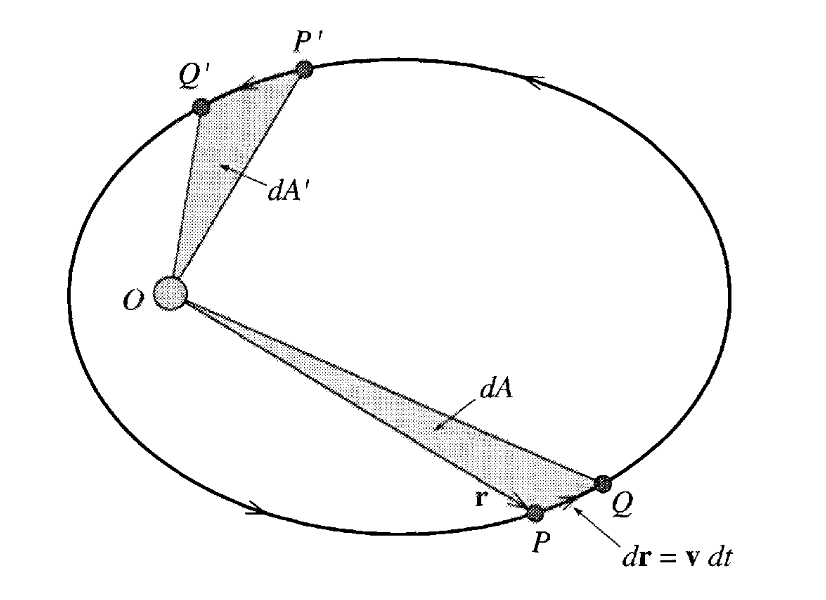
\includegraphics[width=0.5\linewidth]{keplerSecondLaw.png}
    \caption{Kepler's Second Law states that if the two pairs of points $P$, $Q$, $P'$, $Q'$ are separated by equal time intervals $\dd t = \dd t'$, then the two areas $\dd A$ and $\dd A'$ are equal.}
    \label{fig:keplerSecondLaw}
\end{figure}

To show this, we will approximate the area formed by the oval sector $OPQ$ as a triangle with vertices at $O$, $P$, and $Q$. Two of the sides of this triangle can be represented by the vectors $\mbf r$ and $\mbf \dd \mbf r$. Then, recall that the area of the triangle formed by $\mbf r$ and $\dd \mbf r$ is given by
\[ \dd A = \frac{1}{2}\abs{\mbf r \times \dd \mbf r} \]
But since $\dd \mbf r = \mbf v \dd t$, 
\[ \dd A = \frac{1}{2}\abs{\mbf r \times \mbf v \dd t} \]
then, diving by $\dd t$ and replacing $\mbf v$ with $\mbf p/m$,
\[ \frac{\dd A}{\dd t} = \frac{1}{2m}\abs{\mbf r \times \mbf p} = \frac{\ell}{2m} \]
Then, due to the conservation of angular momentum, $\dd A/\dd t$ is constant. This means that Kepler's Second Law is equivalent to the conservation of angular momentum. 

Notice that the proof of Kepler's Second Law depended only on the fact that the gravitational force is central and hence the angular momentum of the planet about $O$ is constant. This means that we can extend these results to any system where an object moves under the influence of just a central force. 
\section{Angular Momentum for Several Particles}
Consider a system of $N$ particles each with angular momentum $\bm{\ell}_i = \mbf{r}_i \times \mbf{p}_i$ relative to some origin $O$. We define the total angular momentum of the system as
\[ \mbf{L} = \sum_i \bm{\ell}_i = \sum_i \mbf{r}_i \times \mbf{p}_i \]
by differentiating with respect to $t$, we find
\begin{equation} \label{ldot1}
    \mbf{\dot L} = \sum_i \bm{\dot \ell}_i = \sum_i \mbf{r}_i \times \mbf{F}_i
\end{equation}
Every object in the system exerts a force on every other object in the system. Therefore, the net force on every particle can be represented as a sum of each internal force, plus the net force on the particle. 
\[ \mbf{F}_i = \sum _{i\neq j} \mbf{F}_{ij} + \mbf{F}^\text{ext}_i \]
Substituting this into (\ref{ldot1}), we find
\[ \mbf{\dot L} = \sum_{i}\sum_{i\neq j} (\mbf{r}_i \times \mbf{F}_{ij}) + \sum_i(\mbf{r}_i \times \mbf{F}^\text{ext}_i) \]
similar to how we worked with linear momentum, we regroup the left sum so it becomes
\begin{align*}
    \mbf{\dot L} &= \sum_i \sum_{j > i}(\mbf{r}_i \times \mbf F_{ij} + \mbf{r}_j \times \mbf F_{ji}) + \sum_i \mbf r_i\times \mbf{F}^\text{ext}_i \\
    &= \sum_i \sum_{j > i}((\mbf{r}_i - \mbf{r}_j)\times \mbf{F}_{ij}) + \sum_i \mbf r_i\times \mbf{F}^\text{ext}_i
\end{align*}
To show that $(\mbf{r}_i \times \mbf{r}_j)\times\mbf{F}_{ij}$, recall that $\mbf{r}_i - \mbf{r}_j$ gives the vector pointing from $\mbf{r}_i$ to $\mbf{r}_j$. Similarly, each force $\mbf{F}_{ij}$ points directly along the line connecting $\mbf{r}_i$ and $\mbf{r}_j$. This means that $\mbf{r}_i - \mbf{r}_j$ is parallel to $\mbf{F}_{ij}$, so their cross product is zero. This allows us to cancel the entirety of the first sum, so we are just left with
\[ \mbf{\dot L} = \sum_i \mbf{r}_i \times \mbf{F}^\text{ext}_i = \sum_i \bm{\Gamma}_i^\text{ext} = \bm{\Gamma}^\text{ext} \]
Therefore, as long as the net external torque of the system is zero, conservation of angular momentum holds for the $N$-particle case.
\begin{theorem}[Principle of Conservation of Angular Momentum]
    If the net external torque on an $N$-particle system is zero, the system's total angular momentum $\mbf L = \sum \mbf{r}_i \times \mbf{p}_i$ is constant.

    In particular, we have $\mbf{\dot L} = \bm{\Gamma}^\text{ext}$.
\end{theorem}
\subsection*{The Moment of Inertia}
The definition of the angular momentum $\mbf{L} = \sum \mbf{r}_i \times \mbf{p}_i$ of a system is certainly valid, but it involves a summation over every particle within the system, which often proves difficult to calculate, especially for rigid bodies which are made up of infinitely many particles of differential mass. To simplify calculations, the notion of a \bf{moment of inertia} was created.

If we take the axis of rotation of the object to be the $z$ axis, then the $z$ component of the angular momentum is given by $L_z = I_z\omega$ where $I_z$ is the moment of inertia of the system about the $z$ axis and $\omega$ is the angular velocity of rotation about the $z$ axis. In general, the moment of inertia about the $z$ axis for a multi-particle system is given by 
\[ I_z = \sum_i m_i r_{iz}^2 \]
where $r_{iz}$ is the distance of the mass $m_i$ from the axis of rotation. 
\subsection*{Angular Momentum about the Center of Mass}
The result $\mbf{\dot L}=\bm{\Gamma}^\text{ext}$ was derived based on the assumption that $\mbf L$ and $\bm{\Gamma}^\text{ext}$ are measured relative to some fixed origin $O$ in an \textit{inertial} reference frame $\mathcal{S}$. Remarkably, the same result holds if $\mbf{L}$ and $\bm{\Gamma}^\text{ext}$ are measured relative to the center of mass of a system--even if the center of mass is being accelerated.

We will prove this result when we look at the mechanics of inertial systems more in depth, but we mention it now as it is a useful result.
\begin{example}[A Sliding and Spinning Dumbbell]
    A dumbbell consisting of two equal masses $m$ mounted on the ends of a rigid massless rod of length $2b$ is at rest on a frictionless horizontal table, lying on the $x$ axis and centered on the origin. At time $t=0$, the left mass is given a sharp tap of force $\mbf{F}$ in the $y$ direction for a short time $\Delta t$. Describe the subsequent motion.

    This problem consists of two parts--the initial motion immediately after the impulse, and the continued motion after the end of the impulse. For the first section, the only force on the object is the applied force from the tap. The linear momentum is initially zero, and because $\mbf{\dot P} = \mbf{F}$, we can integrate to find that at $t=\Delta t$,
    \[ \mbf{P}(\Delta t) = \int_0^{\Delta t} \mbf{F}\dd t = \mbf{F}\Delta t \]
    Furthermore, since $\mbf{P} = M\mbf{\dot R}$, where $M=2m$ is the total mass of the system and $\mbf{R}$ is the position of the position of the center of mass of the system, we can conclude that the center of mass begins to move up the $y$ axis with velocity
    \[ \mbf{\dot R} = \frac{\Delta t}{2m}\mbf{F}\]
    The vector pointing from $\mbf{R}$ to the point of application of the tap is given by $\mbf r = -b\xhat - \mbf{R}$. If we choose the origin to be at the center of mass $\mbf{R}$ and assume that $\Delta t$ is small enough such that $\mbf{R}(t) \approx \mbf{R}(0)$ for $t < \Delta t$, then
    \[ \mbf r \approx -b\xhat \]
    and the torque applied by $\mbf{F}$ relative to the center of mass is approximately constant at
    \[ \mbf{\Gamma} \approx (-b\xhat) \times \mbf{F} = -Fb\zhat \]
    So the angular momentum in the $-\zhat$ direction at $t=\Delta t$ is approximately $L = Fb\Delta t$. This causes a counterclockwise rotation relative to the center of mass. We can then write $L = I\omega$, where $I = \sum m_i r_i^2 = 2mb^2$. This gives
    \[ Fb\Delta t \approx 2mb^2\omega\]
    or $\omega = F\Delta t/2mb$. This means that the left side of the dumbbell is moving with initial velocity
    \[ \mbf{v}_\text{left} = \mbf{\dot R} + \omega b\yhat = \frac{F\Delta t}{m}\yhat  \]
    relative to an outside observer and the right side of the dumbbell is moving with initial velocity
    \[ \mbf{v}_\text{right} = \mbf{\dot R} - \omega b\yhat = \mbf{0} \]
    relative to an outside observer. Thus only the left side of the dumbbell is moving; the right side is initially stationary.

    The subsequent motion is quite straightforward. Once the impulse has ceased, there are no external forces or torques. Thus the center of mass continues to move straight up the $y$ axis with constant speed and the dumbbell continues to rotate with constant angular velocity about the center of mass.
\end{example} % momentum and angular momentum
\chapter{Energy}
\section{Kinetic Energy and Work}
The simplest form of energy is \textbf{kinetic energy} (or KE), which is defined for a particle of mass $m$ moving at velocity $\mbf{v}$ to be
\[ T = \frac{1}{2}m (\mbf{v}\cdot\mbf{v}) = \frac{1}{2}mv^2 =  \]
Imagine the particle moving through space and examine the object's change in kinetic energy as it moves between two neighboring points $\mbf{r}_1$ and $\mbf{r}_1 + \dd \mbf{r}$.  We can differentiate $T$ with respect to time with the product rule for the dot product
\[ \dv{T}{t} = \frac{1}{2}m (\mbf{\dot v} \cdot \mbf{v} + \mbf{v}\cdot\mbf{\dot v}) = m(\mbf{\dot v}\cdot \mbf{v})\]
By Newton's second law $\mbf{F} = m\mbf{\dot v}$, so
\[ \dv{T}{t} = \mbf{F} \cdot \mbf{v} \]
multiplying both sides by $\dd t$ and noting that $\mbf{v}\dd t = \dd\mbf{r}$,
\[ \dd T = \mbf F \cdot \dd \mbf{r} \]
We define the expression $\mbf{F}\cdot \dd\mbf{r}$ as the work done by $\mbf{F}$ as the object undergoes displacement $\dd\mbf{r}$. Thus, the change in a particle's kinetic energy between two neighboring points on its path is equal to the work done by the net force on the particle as it moves between the two points. This is known as the Work-KE theorem.

So far, we've only proven the Work-KE theorem for two infinitesimally close points, but it is relatively simple to generalize to larger displacements. Consider two points $A$ and $B$ with position vectors $\mbf{a}$ and $\mbf{b}$. Suppose a particle follows some path arbitrary path $C$ from $\mbf{a}$ to $\mbf{b}$. We can find the total change in kinetic energy by splitting $C$ into many infinitesimal curves and summing the work across each of them.
\[ \Delta T \equiv T_A - T_B = \lim_{n\to\infty} \sum_{i=1}^n \mbf{F}\cdot \dd \mbf{r_i} \]
this limit can be recognized as approaching the value of the line integral
\[ \Delta T = \int\limits_C \mbf{F}\cdot\dd\mbf{r} \]
as $n\to\infty$. We may also use the alternative notation $\Delta T = \int_A^B\mbf{F}\cdot\dd\mbf{r}$ to represent the same quantity. 

I will also introduce the notation $\int_A^B \mbf{F}\cdot\dd\mbf{r} = W(A\to B)$ to represent the work done as an object moves from $A$ to $B$. 

Another useful property of our definition of work is that the work done by the net force $\mbf{F} = \mbf{F}_1 + \cdots + \mbf{F}_n$ is equal to the sum of the works done by each $\mbf{F}_i$. This result is fairly easy to show.
\begin{align*}
    W(A\to B) &= \int_A^B \mbf{F}\cdot\dd\mbf{r} = \int_A^B \sum_i \mbf{F}_i \cdot \dd \mbf{r} \\
    &= \sum_i \int_A^B \mbf{F}_i \cdot \dd \mbf{r} = \sum_i W_i(A\to B)
\end{align*}
the step between the first and second line is justified by the linearity of the integral. This allows us to write
\begin{equation}\label{workthm}
    \Delta T = \sum_i W_i(A\to B)
\end{equation}
When using the Work-KE theorem, we almost always use it in the form (\ref{workthm})--calculate the work $W_i$ from each individual force acting on the particle, and then set $\Delta T$ equal to their sum. 
\section{Potential Energy and Conservative Forces}
For now, assume that there is just one force acting on the object of interest--this may be the gravitational force between an object and a planet, the electrostatic force on a charged particle in an electric field, an applied force, or really anything else. Depending on the force, it may depend on several different attributes of the object; its velocity, position, time, etc.

We will draw our attention to a particular classification of forces, called \textit{conservative forces}. The properties of these forces will soon become apparent. For a force to be conservative, the first criteria is that it must be solely dependent on the position $\mbf{r}$. For instance, the gravitational force can be written as a function of $\mbf{r}$,
\begin{equation} \label{gforc}
    \mbf{F}(\mbf{r}) = -\frac{GmM}{r^2}\rhat = -\frac{GmM\mbf{r}}{\abs{\mbf{r}}^3}
\end{equation}
Similarly, the electrostatic force on a particle with a non time-dependent electric field is given by $\mbf{F}(\mbf{r}) = q\mbf{E}(\mbf{r})$.

The second condition for a force to be conservative is that the work done between two points $A$ and $B$ must be identical regardless of the path taken between $A$ and $B$. For an example of a force that does not follow this rule, consider the force of friction on an object sliding across the ground. The force is given by
\[ \mbf{F}_\text{fric} = -\mu_k F_N \mbf{\hat v} \]
Because $\dd\mbf{r} = \mbf{v}\dd t$, $\dd \mbf{r}$ is parallel to $\mbf{\hat v}$ and the work is given by
\[ W_\text{fric} = -\mu_k F_N \int_A^B \dd s = -\mu_k F_N \ell \]
where $\ell$ is the length of the path taken from $A$ to $B$. Because two different paths may have different lengths, the work done due to friction is not independent of path, and so friction is not a conservative force. 

For an example of a force that is independent of path, consider the gravitational force. (\ref{gforc}) gives us an expression for $\mbf{F}_\text{grav}$ in terms of $\mbf{r}$. Then,
\begin{align*}
    W_\text{grav} &= -GmM \int_A^B \frac{\mbf{r}}{r^3}\cdot \dd \mbf{r}
\end{align*}
recall from Multivariable Calculus that a line integral is independent of path if and only if the curl of the integrand is $\mbf{0}$. This is true for the gravitational force, as you should verify. 

The name conservative comes from the property that if all forces on the object are conservative, we can define a quantity called the potential energy (PE), denoted $U(\mbf{r})$, a function of only position, with the property that the total mechanical energy
\[ E = T + U(\mbf{r}) \]
is constant. This is known as the principle of conservation of energy, and we will see  how it naturally arises from the below definition of $U$. 

To define the potential energy $U(\mbf{r})$ corresponding to a given conservative force, first choose some reference point $\mbf{r}_0$ where $U$ is defined to be zero. For example, when we analyze gravity near the surface of the Earth, we often define $U$ as zero at ground level. Then, the potential energy at some $\mbf{r}$ is given by
\[ U(\mbf{r}) = -W(\mbf{r}_0\to\mbf{r}) = -\int_{\mbf{r_0}}^{\mbf{r}} \mbf{F}(\mbf{r}')\cdot \dd \mbf{r}' \]
Notice that this definition only makes sense due to the fact that $\mbf{F}$ is conservative--otherwise, we could get several different values for $U(\mbf{r})$ by taking different paths. We will see the reason for the minus sign shortly. 
\begin{example}[Potential Energy of a Charge in a Uniform Electric Field]
    Suppose a charge $q$ is placed in a uniform electric field $\mbf{E} = E_0\xhat$ so that the electric force on $q$ is given by $\mbf{F} = qE_0\xhat$. Show that this force is conservative and find the corresponding potential energy as a function of the position $\mbf{r}$ of the charge. Assume that the gravitational force is negligible.

    The work done by $\mbf{F}$ going between any two points $A$ and $B$ along any path is given by
    \begin{equation} \label{elecconsrv}
        W(A\to B) = \int_A^B \mbf F \cdot \dd \mbf r = qE_0 \int_A^B \xhat \cdot \dd \mbf r = \int_A^B \dd x = qE_0(x_B - x_A)
    \end{equation}
    Because ($\ref{elecconsrv}$) has the same value regardless of the path taken from $A$ to $B$, $\mbf{F}$ is conservative. To define a potential energy, we must define some point where $U=0$. The obvious choice is the origin $\mbf r_0 = \mbf 0$, so
    \[ U(\mbf{r}) = -W(\mbf 0 \to \mbf{r}) = -qE_0 r_x\]
\end{example}

Another critical result can be derived by considering a conservative force $\mbf{F}$ and three points $\mbf{r}_0$, $\mbf{r}_1$, $\mbf{r}_2$, where we define $\mbf{r}_0$ as the reference point where $U(\mbf{r}_0) = 0$. It is easy to convince yourself that
\[ W(\mbf{r}_0 \to \mbf{r}_2) = W(\mbf{r}_0 \to \mbf r_1) + W(\mbf r_1 \to \mbf r_2) \]
which can be rearranged to obtain
\[W(\mbf r_1 \to \mbf r_2) = W(\mbf r_0 \to \mbf r_2) - W(\mbf r_0 \to \mbf r_1)\]
But since $\mbf r_0$ is our reference point, this simply becomes
\[ W(\mbf r_1 \to \mbf r_2) = -(U(\mbf r_2) - U(\mbf r_1)) = -\Delta U \]
This is particularly useful when we combine it with the Work-KE theorem, giving
\[ \Delta T = -\Delta U\]
or
\[ \Delta T + \Delta U = 0\]
In other words, the total mechanical energy $E = T + U$ is conserved. 
\subsection*{Several Forces}
So far we have established the conservation of energy for a particle subject to a single conservative force. We will now see that this result generalizes nicely to an object subject to several conservative forces. For instance, consider a mass suspending from the ceiling by a spring. There are two forces present on the object, the force of gravity $\mbf{F}_\text{grav}$ and the spring force $\mbf{F}_\text{spr}$. As we've already shown, the gravitational force is conservative, and it is relatively easy to see that the force of a spring that obeys Hooke's Law is conservative as well. 
\begin{align*}
    \curl (-k\mbf{r}) = -k (\curl{\mbf r}) = \mbf 0  
\end{align*}
The Work-KE theorem tells us that
\begin{align*}
    \Delta T &= W_\text{grav} + W_\text{spr} \\
    &= -(\Delta U_\text{grav} + \Delta U_\text{spr})
\end{align*}
Rearranging, we obtain $\Delta T + \Delta U_\text{grav} + \Delta U_\text{spr} = 0$, showing that the total mechanical energy of the system is conserved. Similar arguments follow for an arbitrary number of conservative forces.
\begin{theorem}[Principle of Conservation of Energy on a Particle]
    If all of the $n$ forces $\mbf{F}_1, \dots, \mbf{F}_n$ acting on a particle are conservative with a corresponding potential energy $U_1(\mbf{r}), \dots, U_n(\mbf{r}) $, then the total mechanical energy
    \[ E = T + U_1(\mbf{r}) + \cdots + U_n(\mbf{r}) \] 
    is constant.
\end{theorem}
\subsection*{Nonconservative Forces}
If some of the forces on the particle are nonconservative, then we cannot define corresponding potential energies, and we cannot define a conserved mechanical energy. To remedy this, we will split the forces on the object based on whether they are conservative or nonconservative, and we will define the total work done on the object as
\[ W = W_\text{cons} + W_\text{nc}\]
where $W_\text{cons}$ is the work done by all of the conservative forces and $W_\text{nc}$ is the work done by all of the nonconservative forces. This also gives
\[ \Delta T = W_\text{cons} + W_\text{nc} = -\Delta U + W_\text{nc} \]
This can be rearranged to obtain $\Delta T + \Delta U = W_\text{nc}$, or simply $\Delta E = W_\text{nc}$. 

So although mechanical energy is not conserved, it only changes by the amount of work done by all of the nonconservative forces.
\begin{example}[Inclined Plane With Friction]
    Consider a block that starts at rest and begins to slide down a rough incline of angle $\theta$ and coefficient of kinetic friction $\mu_k$.Find the speed $v$ of the object after it as traveled a distance $d$ along the slope. 

    As in the previous inclined plane example (\ref{inclined}), we set up the unit vectors such that $\xhat$ points down the incline and $\yhat$ points normal to the incline. Then, the three forces on the object are 
    \begin{align*}
        \mbf{F} &= \mbf{F}_N + \mbf{F}_\text{grav} + \mbf{F}_\text{fric} \\
        &= (N - mg\cos\theta)\yhat + (mg\sin\theta - \mu_k N)\xhat
    \end{align*}
    Because the net force in the $\yhat$ direction must be zero, we have $N = mg\cos\theta$ and therefore $F_\text{fric} = \mu_k mg \cos \theta$. The gravitational force conservative with potential energy $U = mgh$, where $h$ is the vertical difference between the height where $U=0$ and the current height. We will take $U=0$ to be at the final $h$ value, after the object has slid a distance $d$.

    Through basic trigonometry, this tells us that the height of the initial position of the block relative to the final position is $h_0 = d\sin\theta$, and therefore
    \[ \Delta U = -mgd\sin\theta \]
    
    The normal force does not do any work on the particle (as it is perpendicular to the velocity which solely points in the $\xhat$ direction).  

    Because the frictional force is always antiparallel to the velocity vector, we have
    \[ W_\text{nc} = W_\text{fric} = -\mu_k dmg\cos\theta \]
    Finally, the kinetic energy of the particle is simply $T = \frac{1}{2}mv^2$, as always. Because the object is initially at rest, the initial kinetic energy is zero and $\Delta T = T$. Then, since $\Delta T + \Delta U = W_\text{nc}$, we have
    \[ \frac{1}{2}mv^2 - mgd\sin\theta = -\mu_k dmg\cos\theta \]
    which can be rearranged to find
    \[ v = \sqrt{2gd(\sin\theta-\mu_k \cos\theta)}\]
\end{example}
\section{Force as the Gradient of Potential Energy}
Previously, we wrote the potential energy $U(\mbf{r})$ of a particle undergoing conservative forces as a type of integral of the force $\mbf{F}(\mbf{r})$. Now, it seems natural to write the force as some form of derivative of the potential energy. To begin, the change in potential energy as an object moves from $\mbf r$ to $\mbf r + \dd \mbf r$ is, by definition
\[ \dd U = U(x + \dd x, y + \dd y, z + \dd z) - U(x, y, z) \]
Just as we can write $f(x + \dd x) - f(x) = \dv{f}{x}\dd x$ for functions of a single variable, we can write
\begin{align}
    \dd U &=  U(x + \dd x, y + \dd y, z + \dd z) - U(x, y, z) \nonumber \\
    &= \pdv{U}{x}\dd x + \pdv{U}{y}\dd y + \pdv{U}{z}\dd z \label{du1}
\end{align}
We can also write 
\begin{align}
    \dd U &= -\int_{\mbf r}^{\mbf r + \dd r} \mbf{F}(\mbf{r}') \cdot \dd \mbf{r}' \approx -\mbf{F}(\mbf{r})\cdot \dd \mbf{r} \nonumber \\
    &= -\pqty{F_x\dd x + F_y\dd y + F_z\dd z } \label{du2}
\end{align}
By equating (\ref{du1}) and (\ref{du2}), we obtain
\[ \pqty{\pdv{U}{x} + F_x}\dd x + \pqty{\pdv{U}{y} + F_y}\dd y + \pqty{\pdv{U}{z} + F_z}\dd z = 0\]
To simplify this equation somewhat, imagine the special case where the object is only moving in the $x$ direction; in other words, $\dd y = \dd z = 0$. This gives $F_x + \partial U/\partial x = 0$ or $F_x = -\partial U/\partial x$. Repeating this process for the $y$ and $z$ coordinates, we find
\[ F_x = -\pdv{U}{x} \quad F_y = -\pdv{U}{y} \quad F_z = -\pdv{U}{z} \]
In vector form, this equation can be simply written as 
\[ \mbf{F} = -\nabla U \]
One thing to note is that this whole analysis hinges upon the fact that $\mbf{F}$ is conservative. In other words, conservative forces are always derivable from a potential energy. 
\begin{example}[Finding a Force From a Potential Energy]
    The potential energy of a particle is given by $U = Axy^2 + B\sin Cz$ where $A,B,C\in\R$ are arbitrary. Find the corresponding force field.
    
    To find $\mbf{F}$, we simply compute the gradient of $U$ and multiply it by $-1$.
    \[ \mbf{F} = -\nabla U = -Ay^2\xhat - 2Axy\yhat - BC\cos(Cz)\zhat \]
\end{example}
Another useful relationship that we will take advantage of is the fact that
\[ \dd U = \nabla U \cdot \dd \mbf{r} \]
This is a general property of the gradient that we may also apply in other scenarios as well.
\section{Time-Dependent Potential Energy}
Consider a force $\mbf{F}(\mbf{r}, t)$ that satisfies $\curl\mbf{F} = \mbf 0$. This field is still conservative in the mathematical sense--there exists some potential $U(\mbf{r},t)$ such that $\mbf F = -\nabla U$. But because there is a time dependency, it is no longer the case that the total mechanical energy $E = T + U$ is conserved.

As a sidenote, the $\nabla$ operator is still defined as $\langle \partial_x, \partial_y, \partial_z \rangle$ when working with time-dependent fields--that is, we only consider the spatial coordinates in operations involving $\nabla$.

For an example of a field of this type, consider a conducting sphere with a non-constant charge $Q(t)$--for instance, suppose the sphere is connected by a rod with non-negligible resistance to the ground, causing charge to slowly leak into the ground.

It is relatively easy to show that the force $\mbf{F}_\text{elec}$ exerted on a small charge $q$ is non-constant, but satisfies $\curl \mbf{F}_\text{elec}(\mbf r, t) = \mbf 0$ for all $\mbf{r}$ and $t$. 

To show that a potential energy function indeed exists, recall that $\curl\mbf{F}(\mbf r, t) = 0$ tells us that any line integral of $\mbf{F}$ is dependent only on the endpoints (path independence). Therefore, we can define $U(\mbf{r}, t)$ as
\[ U(\mbf{r},t) = -\int_{\mbf{r_0}}^{\mbf{r}} \mbf{F}(\mbf{r}', t)\cdot \dd \mbf{r}' \]
where $\mbf{r}_0$ is some sample point where we define $U(\mbf{r}, t) =0$. Using the same methods as in the previous section, we can show that $\mbf{F}(\mbf{r}, t) = -\nabla U(\mbf{r}, t)$.

So far, everything is identical to the behavior of $U$ with no time dependence, but now the story changes. We define the total mechanical energy $E = T + U$, as usual. Consider two nearby points in time $t$ and $t + \dd t$. The change in kinetic energy $T$ is given by
\begin{align} \label{dt,td}
    \dd T = \dv{T}{t}\dd t = m(\mbf{\dot v} \cdot \mbf{v})\dd t = \mbf{F}\cdot \dd \mbf{r} 
\end{align}
and the change in potential energy $U$ is given by
\[ \dd U = \pdv{U}{x}\dd x + \pdv{U}{y}\dd y + \pdv{U}{z}\dd z + \pdv{U}{t}\dd t \]
The first three terms on the left can be recognized as $\nabla U \cdot \dd \mbf{r} = -\mbf{F}\cdot\dd\mbf{r}$. Therefore,
\begin{equation} \label{du,td}
    \dd U = -\mbf{F}\cdot\dd\mbf{r} + \pdv{U}{t}\dd t
\end{equation}
The total change in mechanical energy is the sum of (\ref{dt,td}) and (\ref{du,td}):
\[ \dd E = \pdv{U}{t}\dd t\]
Clearly, the mechanical energy $E$ is only conserved when $U$ is independent of $t$; that is, when $\partial U/\partial t = 0$. 

\section{Energy in Linear One-Dimensional Systems}
So far we have only discussed energy for a particle that is free to move in all three spatial dimensions. Many interesting and important problems involve an object that is constrained to move in just one dimension, and the methods to analyze these problems is much simpler than the more general case. 

We are used to the notion of a one-dimensional system as a perfectly straight, or linear, track. In discussing these types of linear systems, we take the $x$ axis to coincide with the track, and the position of the object is specified by a single coordinate $x$. There are much more complicated linear systems, however. Consider a roller coaster following a track; the system is still one dimensional, although it is not linear.

In this section, we will focus solely on linear one-dimensional systems, although we will soon see that analysis of nonlinear one-dimensional systems does not differ from analysis of their linear counterparts as much as one might expect.

To begin, consider an object constrained to move along a perfectly straight track, which we take to be the $x$ axis. The only component of any force $\mbf{F}$ that can do any work is the $x$ component, and so we can simply ignore the other components. Thus, the work is given by
\begin{equation} \label{work1d}
    W(x_1\to x_2) = \int_{x_1}^{x_2} F_x(x)\; \dd x
\end{equation}
As before, for $F_x$ to be conservative, it must satisfy the following two conditions:
\begin{enumerate}
    \item The force $F_x$ depends only on the position $x$.
    \item The integral (\ref{work1d}) is independent of path.
\end{enumerate}
For one-dimensional systems, however, the first condition implies the second so the second condition can be disregarded altogether.

For the first condition, notice that despite the fact that we are in one dimension only, there are still many possible paths from $x_1$ to $x_2$. There is, of course, the straight path that takes us directly from $x_1$ to $x_2$. But then, consider another path that goes from $x_1$ to $x_2$ and then \textit{continues} going to another point $x_3$ that is past $x_2$, before doubling back and returning to $x_2$. The work done along this path is described by
\[ W(x_1\to x_2 \to x_3\to x_2) = W(x_1\to x_2) + W(x_2\to x_3) + W(x_3\to x_2) \]
Provided the force $F_x$ is only dependent on the position $x$, we have
\begin{align*}
    W(x_3\to x_2) &= \int_{x_3}^{x_2}F_x(x)\; \dd x = -\int_{x_2}^{x_3} F_x(x) \; \dd x = -W(x_2\to x_3)
\end{align*}
Thus the $W(x_2\to x_3)$ and $W(x_3\to x_2)$ terms cancel and we simply have
\[ W(x_1\to x_2\to x_3 \to x_2) = W(x_1\to x_2)\]
These same principles can be applied to paths that double back on themselves arbitrarily many times before finally reaching their final destinations, showing that the work is fully independent of path. 
\subsection*{Graphs of the Potential Energy}
A second useful feature of one-dimensional system is that we can graph the potential energy $U(x)$ as a function of only one variable, making visualization a much easier task than it would be in several dimensions.

Assuming all forces acting on an object are conservative, we can write
\[ U(x) = U(x_0)-\int_{x_0}^x F_x(x')\; \dd x'\]
We often choose $x_0$ such that $U(x_0) = 0$, causing the left term to go away.

For instance, if a mass is attached to a spring obeying Hooke's Law, we have $F_x(x) = -kx$, so choosing $x_0=0$ to be the location with zero potential energy,
\begin{align*}
    U(x) &= -\int_0^x F_x(x')\; \dd x' \\
    &= k\int_0^x x' \; \dd x' = \frac{1}{2}kx^2 
\end{align*}
The one-dimensional analogue to the relationship $\mbf{F} = -\nabla U$ is the comparatively simple result
\[ F_x = -\dv{U}{x} \]

Plotting the potential energy against $x$ allows us to qualitatively analyze how the object must behave. The direction of the net force is the opposite of the slope of the graph of $U(x)$, so the object will naturally tend to accelerate ``downhill" on the graph.
\begin{figure}[h!]
    \centering
    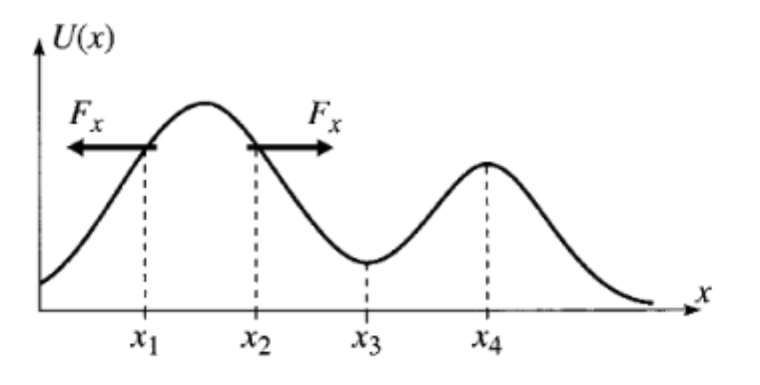
\includegraphics[width=0.5\linewidth]{potentialEnergy1d.png}
    \label{fig:U1d}
\end{figure}
At locations such as $x_3$ and $x_4$ where the graph has an extremum, the net force on the object is zero and so the object may remain in equilibrium there (provided it is initially stationary). Depending on whether the extrema is a local minimum or maximum, we call it either a \textit{stable equilibrium} (local minimum) or an \textit{unstable equilibrium} (local maximum). To justify this, imagine an object stationary at a stationary equilibrium such as $x_3$ on the above graph. If it receives a small perturbation in either direction, it will tend to accelerate back towards the equilibrium point. If it were instead at an unstable equilibrium such as $x_4$ on the above graph, a small perturbation would cause the object to continually accelerate away from the equilibrium point.

Some graphs may have an extremum that is stable in one direction and unstable in the other--we call these \textit{semi-stable equilibrium} points. These are rarer than stable or unstable equilibrium points, but one example would be at $x=0$ if we had $U(x) = x^3$.

We can also study these objects' behavior with the conservation of energy. Suppose at some point $x=x_0$, we have
\[ E = T(x_0) + U(x_0) \]
Because $E$ is constant, we then necessarily have, for any point $x_1$,
\[ T(x_1) + U(x_1) = T(x_0) + U(x_0) \]
Suppose that $x_1 > x_0$ and there exists some $b$ such that $x_0 < b < x_1$ and
\[ U(b) = T(x_0) + U(x_0) \]
Then, it is \textit{impossible} for the object to pass $x = b$ without an external force, as that would require it to possess some kinetic energy there. But we know this cannot be the case, as 
\[ U(b) + T(b) = T(x_0) + U(x_0)  \]
implying $T(b) = 0$. In this case, we call $x=b$ a \textit{turning point} for the motion of the object, provided it is not an equilibrium point, as it causes the object to turn around and begin accelerating in the opposite direction.

One insightful way to visualize the locations of these turning points is to draw a horizontal line at $U(x) = E$, such as the graph below.
\begin{figure}[h!]
    \centering
    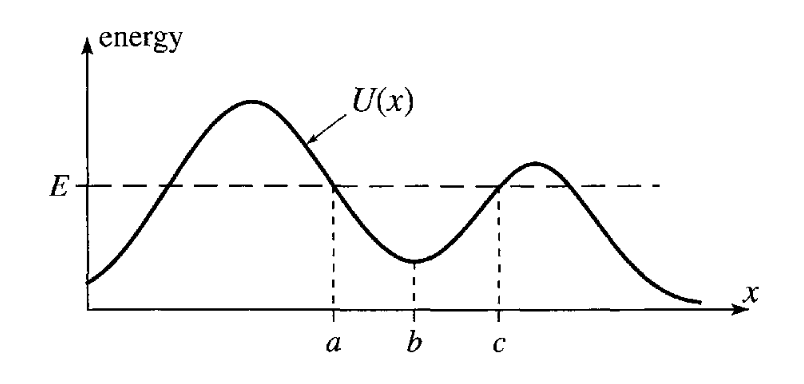
\includegraphics[width=0.5\linewidth]{potentialEnergy1d_2.png}
    \label{fig:U1d2}
\end{figure}

any point above the dashed horizontal line cannot be reached without some non-conservative force increasing the total energy of the particle (this is unlikely, as non-conservative forces typically dissipate energy rather than increase it).

Further, if the object ever enters the area between $x=a$ and $x=c$, it will continue to oscillate between them indefinitely--it can never escape this ``well" as that would require it have enough energy to overcome the crest of the hills on either side, which it simply doesn't. If the object has enough energy to overcome the crest on the right side, but not the crest on the left side, we can guarantee that it will escape to the right. If it has enough energy to overcome both crests, it could escape in either direction.
\subsection*{Complete Solution of the Motion}
Another remarkable feature of one-dimensional conservative systems is that we can use the conservation of energy to obtain a complete solution of the motion, as long as we know the total energy $E$ and the potential energy $U(x)$.

The equation $\frac{1}{2}m\dot{x}^2 + U(x) = E$ can be rearranged to give
\[ \dot x = \pm \sqrt{\frac{2}{m}(E-U(x))}\]
The sign ambiguity comes from the fact that kinetic energy is the same regardless of the direction of $\dot x$. 

This is a first order autonomous differential equation that can be solved through separation of variables, giving

\[ \sqrt{\frac{m}{2}}\int_{x_0}^x \frac{\dd x'}{\sqrt{E-U(x)}} = t - t_0\]
where $x(t_0) = x_0$.
\section{Curvilinear One-Dimensional Systems}
We will now turn our attention to the other type of linear system I mentioned--systems where the path may not be straight.

Instead of defining the position in terms of a distance $x$ along an axis, we will define it in terms of an arc-length $s$ along the curve. To develop equations describing the path, we will consider two frameworks to analyze its motion. First, there is the one dimensional perspective we have just laid out, where position is measured in terms of the arclength $s$. However, we can also talk about the position of the particle in terms of its $x$ and $y$ components. These systems are related with the line integral 
\[ s = \int\limits_C \dd s'\]
Where $C$ is the curve going from the point we have denoted $s=0$ to the point at which we are measuring $s$. We can also write
 \[ \dd s = \sqrt{\dd x^2 + \dd y ^2} \]
 or
 \[ \dot s = \sqrt{\dot x^2 + \dot y^2}\]
 Recognizing $\sqrt{\dot x^2+\dot y^2}$ as the speed of the particle, this tells us that in terms of arclength, the speed is simply $\dot s$. We can then write the kinetic energy as
\[ T = \frac{1}{2}m\dot s^2\]
As for the force, we will consider it as the sum of a normal component and a tangential component. The normal component is often called the \textit{force of constraint} as it is what causes the particle to remain on the path--if we consider osculating circle to the curve, we can imagine the normal component as a type of centripetal force keeping the object along the ever-changing circular path. 

Because the normal component is perpendicular to the path of the particle, it does no work on it. Further, we have $m\ddot{s} = F_\text{tan}$. To show this, first note the relationship $v^2 = \dot s^2 = \mbf{v} \cdot \mbf{v}$. Taking the time derivative of each side, we find
\begin{align*}
    \dot{s}\ddot{s} = \mbf{v} \cdot \mbf{\dot v}
\end{align*}
if we write the net force vector as 
\[ \mbf{F} = F_\text{tan}\mbf{\hat{T}} + F_\text{N} \mbf{\hat N}\]
where $\mbf{\hat{T}}$ is the unit tangent vector to the curve and $\mbf{\hat{N}}$ is the unit normal vector to the curve, we get
\[ \mbf{\dot v} = \frac{1}{m} (F_\text{tan}\mbf{\hat{T}} + F_\text{N} \mbf{\hat N}) \]
or
\[ m\dot{s}\ddot{s} = F_\text{tan}\mbf{v} \cdot \mbf{\hat{T}} + F_\text{N} \mbf{v}\cdot \mbf{\hat N} \]
Because the velocity is always parallel to the tangent vector and orthogonal to the normal vector, $\mbf{v}\cdot\mbf{\hat T} = v = \dot s$ and $\mbf{v}\cdot\mbf{\hat N} = 0$. Therefore,
\[ m\ddot{s} = F_\text{tan}\]
as desired. 

If all of the forces on the particle with a tangential component are conservative, we can define a potential energy $U(s)$ with
\[ U(s) = \int_{s_0}^s F_\text{tan}(s')\; \dd s'\]
similar to the potential energy in linear one-dimensional systems, we have $F_\text{tan} = -\dd U/\dd s$ and we can apply the entirety of our previous discussion about the graphs of $U$ to curvilinear coordinates without many changes.

\begin{example}[Stability of a Cube Balanced on a Cylinder]
    
    \begin{minipage}{0.48\textwidth}
        A hard rubber cylinder of radius $r$ is held fixed with its axis horizontal, and a cube of mass $m$ and sidelength $2b$ is balanced on top of the cylinder, with its center vertically about the cylinder's axis and four of its sides parallel to the axis. The cube cannot slip on the rubber of the cylinder, but it can rock from side to side. Determine if the equilibrium of the cube centered above the cylinder is stable. 

        This system seems complicated, but it is in fact a one-dimensional system in terms of the angle $\theta$ formed between the vertical and the side of the box pointing up. The forces acting on the box are the normal force between it and the cylinder and the gravitational force acting on the box. If we define $h=0$ to be at the height of the axis of the cylinder, we know that the gravitational potential energy is given by $U = mgh$.
    \end{minipage}
    \begin{minipage}{0.48\textwidth}
        \parbox{\textwidth}{
            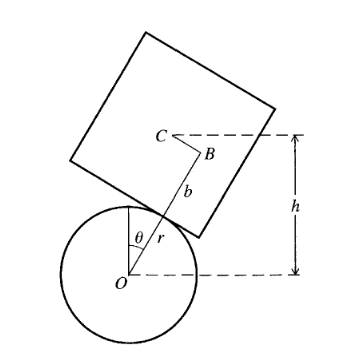
\includegraphics[width=\textwidth]{cubeOnCylinder.png}
        }
    \end{minipage}
    
    With some geometry, we can see that
    \[ h = (r+b)\cos\theta + r\theta\sin\theta \]
    The $r\theta\sin\theta$ term originates from the fact that the length of the line segment $BC$ is the amount the cube has rolled down the cylinder, namely $r\theta$, and the component of that in the vertical direction is $r\theta\sin\theta$.

    Therefore the potential energy as a function of $\theta$ is given by
    \[ U(\theta) = mg((r+b)\cos\theta + r\theta\sin\theta) \]
    and its derivative is 
    \begin{align*}
        \dv{U}{\theta} &= mg(r\sin\theta + r\theta\cos\theta - (r+b)\sin\theta) \\
        &= mg(r\theta\cos\theta - b\sin\theta) 
    \end{align*}
    Equilibrium occurs at the point where $\dd U/\dd \theta = 0$, or when $r\theta\cos\theta = b\sin\theta$. The nonzero solutions to this equation cannot be found analytically, and whether or not a nonzero solution even exists will depend on the $b$ and $r$ values. For the solution where $\theta = 0$, however, we can determine the stability with the second derivative test.
    \begin{align*}
        \dv[2]{U}{\theta} = mg((r-b)\cos\theta - r\theta\sin\theta)
    \end{align*}
    and when $\theta =0$,
    \[ \dv[2]{U}{\theta}\biggr|_{\theta = 0} = mg(r-b)\]
    Therefore the equilibrium at $\theta = 0$ is stable if $r > b$ and unstable if $r < b$. If $r=b$, the second derivative reduces to
    \[ \dv[2]{U}{\theta} = -r\theta\sin\theta\]
    and the second derivative test is inconclusive. We will have to differentiate again (twice, actually--the third derivative turns out to be zero as well) to find that $\theta = 0$ is an unstable equilibrium. 
\end{example}
\subsection*{Further Generalizations}
Many other complicated systems can still be described as one-dimensional. Such systems may comprise of many bodies joined together by strings or springs in such a way that just one parameter is needed to describe the position of the system. For instance, consider the Atwood machine consisting of two masses $m_1$ and $m_2$ suspended from a frictionless pulley. We will assume the pulley is massless here, although it doesn't have to be. The masses can move up and down, but the forces of the puller on the string and the string on the masses constrain matters so that the mass $m_2$ can only move down by exactly the amount the $m_1$ moves up (or vice versa).

Thus the whole system can be specified by a single parameter. Here, we will choose the height $x$ of $m_1$ below the pulley's center. All forces on the system are conservative so we have
\[ \Delta T_1 + \Delta U_1 = W_1^\text{ten} \]
and
\[ \Delta T_2 + \Delta U_2 = W_2^\text{ten} \]
In the absence of friction, the tension is the same all along the string, so $F_1^\text{ten} = -F_2^\text{ten}$ and
\[ W_1^\text{ten} = -W_2^\text{ten} \]
implying
\[ \Delta (T_1 + U_1 + T_2 + U_2) = 0\]
or, in other words, the total energy of the system is conserved. 

It turns out that many systems of this type, where several particles are present but are constrained in some way so they must move by the same amounts. The forces of constraint are important in the behavior of each individual particle, but when all added together do no net work on the system. Thus we can define a \textit{conserved} total energy
\[ E = \sum_\alpha (T_\alpha + U_\alpha) \]
\section{Central Forces}
A three-dimensional scenario with some of the simplicity of one-dimensional problems is a particle subject to a central force. If the center of the force is the origin, a central force has the form
\[ \mbf{F}(\mbf{r}) = f(\mbf{r})\rhat \]
where the function $f(\mbf{r})$ gives the magnitude of the force, with positive values if the force points radially out or negative values if the force points radially in. For instance, consider the Coulomb force between two charges
\[ \mbf{F}_E(\mbf{r}) = \frac{kQq}{r^2}\rhat \]
The Coulomb force has two additional properties that not all central forces contain--it is conservative, as we have already shown, and it is \textbf{spherically symmetric} or \textbf{rotationally invariant}; that is, the magnitude function $f(\mbf{r})$ is independent of the direction of $\mbf{r}$ and hence can be written as purely a function of the magnitude of $\mbf{r}$:
\[ f(\mbf{r}) = f(r) \]
Remarkably, any central force that is conservative is rotationally invariant, and vice versa. Before we show why this is the case, it will be useful to give a brief review of the gradient in spherical polar coordinates
\subsection*{The Gradient in Spherical Polar Coordinates}
We know the gradient of a scalar field in cartesian coordinates to be 
\[ \nabla f = \pdv{f}{x}\xhat + \pdv{f}{y}\yhat + \pdv{f}{z}\zhat \]
In spherical coordinates, this statement is not quite as simple. To find it, consider a small displacement $\dd \mbf{r}$. This displacement causes a change in $f$ given by
\begin{equation} \label{df}
    \dd f = \nabla f \cdot \dd \mbf{r}
\end{equation}
If $\dd \mbf{r} = \alpha \rhat +  \beta \bm{\hat{\theta}} + \gamma \bm{\hat\phi}$, we can use some geometry to determine the coefficients $\alpha, \beta,\gamma$ in terms of the changes $\dd r, \dd \theta, \dd \phi$. 

A small change in $r$ causes a movement $\dd r$ radially outward. A small change in $\theta$ causes a movement along the $\theta$ circle given by $r\dd \theta$, and a small change in $\phi$ causes a movement along the $\phi$ circle given by
\[ (\text{projection of $\dd \mbf{r}$ onto the $xy$ plane})\; \dd \phi = r\sin\theta \dd \phi \]
In other words,
\[ \dd \mbf{r} = \dd r \rhat + r\dd \theta \bm{\hat\theta} + r\sin\theta \bm{\hat\phi} \]
Plugging this into (\ref{df}), we obtain
\[ \dd f = (\nabla f)_r\,  \dd r + (\nabla f)_\theta r\, \dd \theta + (\nabla f)_\phi r\sin\theta \, \dd \phi \]
Meanwhile, since $f$ is a function of three variables, we can use the chain rule to obtain
\[ \dd f = \pdv{f}{r}\dd r + \pdv{f}{\theta}\dd\theta + \pdv{f}{\phi}\dd\phi \]
comparing the components of these two expressions of $\dd r$, we find
\[ (\nabla f)_r = \pdv{f}{r}, \quad (\nabla f)_\theta = \frac{1}{r}\pdv{f}{\theta}, \quad (\nabla f)_\phi = \frac{1}{r\sin\theta}\pdv{f}{\phi}  \]
or,
\[ \nabla f = \pdv{f}{r}\rhat + \frac{1}{r}\pdv{f}{\theta} \bm{\hat\theta} + \frac{1}{r\sin\theta}\pdv{f}{\phi} \bm{\hat\phi} \]
similar considerations must be applied when considering the curl and divergence in spherical coordinates. 

Specifically, we can see that the curl of a vector field in spherical coordinates is given by
\[ \nabla \times \mbf{F} = \frac{1}{r^2\sin\theta}\begin{vmatrix}
    \rhat & r\bm{\hat\theta} & r\sin\theta \bm{\hat\phi} \\
    \pdv{r} & \pdv{\theta} & \pdv{\phi} \\
    F_r & rF_\theta & r\sin\theta F_\phi
\end{vmatrix} \]
The proof of this is simple but tedious, so it is left as an exercise. 
\subsection*{Conservative and Spherically Symmetric, Central Forces}
I previously claimed that a central force is conservative if and only if it is spherically symmetric. If $\mbf{F}$ is conservative, its curl is zero. Suppose $\mbf{F}$ is central and conservative. Then,
\begin{align*}
    \nabla \times\mbf{F} &= \frac{1}{r^2\sin\theta}\begin{vmatrix}
    \rhat & r\bm{\hat\theta} & r\sin\theta \bm{\hat\phi} \\
    \pdv{r} & \pdv{\theta} & \pdv{\phi} \\
    F_r & rF_\theta & r\sin\theta F_\phi
\end{vmatrix} \\
&= \frac{1}{r^2\sin\theta}\pqty{r\cos\theta F_\phi + r\sin\theta \pdv{F_\phi}{\theta} - r\pdv{F_\theta}{\phi}}\rhat \\
&- \frac{1}{r^2\sin\theta}\pqty{r\sin\theta F_\phi + r^2 \sin\theta \pdv{F_\phi}{r} - r\pdv{F_r}{\phi}}\bm{\hat\theta} \\
&+ \frac{1}{r^2\sin\theta}\pqty{r\sin\theta F_\theta + r^2\sin\theta \pdv{F_\theta}{r} - r\sin\theta \pdv{F_r}{\theta}}\bm{\hat\phi} = \mbf{0}
\end{align*}
We can multiply away the factor of $1/(r^2\sin\theta)$ and note that because $\mbf{F}$ is central, $F_\theta$ and $F_\phi$ are both just zero. This gives
\begin{align*}
    \nabla \times \mbf{F} &= 0\rhat + r\pdv{F_r}{\phi}\bm{\hat\theta} - r\sin\theta \pdv{F_r}{\phi}\bm{\hat\phi}
\end{align*}
Because $\nabla\times\mbf{F} = \mbf{0}$, we have
\[ \pdv{F_r}{\phi} = \pdv{F_r}{\theta} = 0\]
meaning that $\mbf{F}$ is not dependent on $\phi$ or $\theta$; it is rotationally invariant, as desired.

For the proof in the reverse direction, suppose $\mbf{F}$ is central and rotationally invariant. Then, we follow the same process to find
\begin{align*}
    \nabla \times \mbf{F} &= 0\rhat + r\pdv{F_r}{\phi}\bm{\hat\theta} - r\sin\theta \pdv{F_r}{\phi}\bm{\hat\phi}
\end{align*}
Because $\mbf{F}$ is rotationally invariant, its partials with respect to $\phi$ and $\theta$ are zero, so $\nabla\times\mbf{F} = \mbf{0}$, and $\mbf{F}$ is conservative.

\section{Energy of the Interaction Between Two Particles}
Before we can consider the energy of a many-particle system, we'll start with the reduced case where there are only two particles. Suppose two particles exert forces $\mbf{F}_{12}$ and $\mbf{F}_{21} = -\mbf{F}_{12}$ on each other. In general, $\mbf{F}_{12}$ may depend on the locations $\mbf{r}_1$ and $\mbf{r}_2$ of the particles, so
\[ \mbf{F}_{12} = \mbf{F}_{12}(\mbf{r}_1, \mbf{r}_2) \]
for instance, consider two objects in space (which I will label $1$ and $2$) that exert a gravitational force on each other. The force on $1$ by $2$ is
\[ \mbf{F}_{12}(\mbf{r}_1, \mbf{r}_2) = -\frac{GMm}{\abs{\mbf{r}_1-\mbf{r}_2}^3}(\mbf{r}_1-\mbf{r}_2) \]
Notably, the force only depends on the \textit{difference} between the positions of $1$ and $2$, not the actual positions themselves. This property, known as \textbf{translational invariance}, is not a coincidence, and is in fact a property of any isolated two-particle system; if we pick up the entire system and move it elsewhere, retaining the relative distances between the particles, the forces will not change. If we define the displacement vector $\mbf{r} = \mbf{r}_1 - \mbf{r}_2$, we can write
\[ \mbf{F}_{12}(\mbf{r}) = -\frac{GMm}{\abs{\mbf{r}}^3}\mbf r\]
To analyze this system, let us fix particle 2's location at some constant point--we will use the origin for convenience. Then, $\mbf{r} = \mbf{r}_1$ and our discussion of forces on a single particle apply. For instance, if the force $\mbf{F}_{12}$ is to be conservative, it must satisfy
\[ \nabla_1 \times \mbf{F}_{12} = \mbf 0\]
where $\nabla_1 = \pdv{x_1} \xhat + \pdv{y_1}\yhat + \pdv{z_1}\zhat$ is the differential operator with respect to the coordinates $(x_1, y_1, z_1)$ of particle $1$. If $\mbf{F}_{12}$ is conservative, then we can define a potential energy
\[ \mbf{F}_{12} = -\nabla_1 U(\mbf{r}_1) \]
If we wish to find the potential energy with $\mbf{r}_2$ fixed at some other point, we simply translate the whole system so
\[ \mbf{F}_{12} = -\nabla_1 U(\mbf{r}_1 - \mbf{r}_2) \]
To find the reaction force $\mbf{F}_{21}$, simply invoke Newton's Third Law,
\[ \mbf{F}_{21} = -\mbf{F}_{12} = \nabla_1U(\mbf{r}_1-\mbf{r}_2) = -\nabla_2 U(\mbf{r}_1-\mbf{r}_2) \]
where the last equality holds from the chain rule. This shows an important result: for the interaction between two particles, there is a \textit{single} potential energy function $U$, from which both forces can be derived. 

Before moving on to a discussion of multiparticle systems, consider a two-particle system where in a small period of time $\dd t$, particle 1 moves a distance $\dd \mbf{r}_1$ and particle 2 moves a distance $\dd \mbf{r}_2$. The Work-KE theorem tells us that
\[ \dd T_1 = (\text{work on 1}) = \dd \mbf{r}_1 \cdot \mbf{F}_{12} \]
and
\[ \dd T_2 = (\text{work on 2}) = \dd \mbf{r}_2 \cdot \mbf{F}_{21} = -\dd \mbf r_2 \cdot \mbf{F}_{12}\]
So the net change in kinetic energy for the system is
\[ \dd T = \dd T_1 + \dd T_2 = \dd (\mbf r_1 - \mbf r_2) \cdot \mbf{F}_{12} = \dd(\mbf r_1 - \mbf r_2) \cdot (-\nabla_1U(\mbf r_1-\mbf r_2)) = -\dd U\]
In other words, $\dd T + \dd U = 0$, so the total mechanical energy of the system is conserved. 

The key observation here is that instead of a potential energy for \textit{both} $\mbf{F}_{12}$ and $\mbf{F}_{21}$, there is one potential energy describing the entire interaction between particle 1 and particle 2, from which both forces can be derived.

\subsection*{Elastic Collisions}
One application of these ideas arises in the study of \textit{elastic collisions}. An elastic collision is a collision between two particles that interact only via conservative forces that go to zero as their separation $\mbf r_1 - \mbf r_2$ increases. Because the forces go to zero, the potential energy approaches a constant which we may as well take to be zero.

Because all forces involved in the collision are conservative, the total mechanical energy remains constant. In other words
\[ U_0 + T_0 = U_f + T_f\]
because the objects start far away initially and will be separated again after the collision, both $U_0$ and $U_f$ are zero, so
\[ T_0 = T_f \]
can be used to completely solve for the motion of the system. 
\begin{example}[An Equal-Mass Elastic Collision]
    Consider an elastic collision between two particles with equal mass $m$. One of the particles is initially at rest and the other is approaching with a velocity $\mbf v_1$. Show that the angle between the outgoing velocities of each ball is $\theta = 90^\circ$.

    To show this, we can first set up a conservation of energy equation:
    \[ \frac{1}{2}m\mbf v_1 \cdot \mbf v_1 = \frac{1}{2}m\mbf v_1' \cdot \mbf v_1' + \frac{1}{2}m\mbf v_2' \cdot \mbf v_2'\]
    The factor of $m/2$ cancels so
    \begin{equation} \label{cnsvener}
        \mbf v_1 \cdot \mbf v_1 = \mbf v_1' \cdot \mbf v_1' + \mbf v_2' + \mbf v_2'
    \end{equation}
    Additionally, conservation of momentum tells us that
    \begin{equation} \label{v1inprimes}
        \mbf v_1 = \mbf v_1' + \mbf v_2' 
    \end{equation}
    Substituting (\ref{v1inprimes}) into (\ref{cnsvener}), we find
    \[ \mbf v_1' \cdot \mbf v_1' + 2\mbf v_1' \cdot \mbf v_2' + \mbf v_2' \cdot \mbf v_2' = \mbf v_1' \cdot \mbf v_1' + \mbf v_2' + \mbf v_2'\]
    This tells us that $\mbf v_1' \cdot \mbf v_2' = 0$, so they are perpendicular, as desired.
\end{example}
\section{The Energy of a Multiparticle System}
We will now extend our discussion of energy to systems with many particles.

Consider a system of $N$ particles where each particle exerts a conservative force $\mbf F_{\alpha\beta}$ on each other particle, and each particle has some net external force $\mbf F_\alpha^\text{ext}$. 

First, we can immediately define the net kinetic energy of the system as the sum of each particle's individual kinetic energy
\[ T = \sum_\alpha \frac{1}{2}m_\alpha v_\alpha^2\]
Each interparticle force can be written as
\[ \mbf F_{\alpha \beta} (\mbf r_\alpha - \mbf r_\beta) = -\nabla _\alpha U_{\alpha\beta}(\mbf r_\alpha - \mbf r_\beta) \]
where each pair of particles has a potential energy describing their interaction. We define the total internal potential energy as the sum of each of these potential energies:
\[ U^\text{int} = \sum_\alpha \sum _{\beta > \alpha} U_{\alpha\beta} \]
Each particle also has some external force $\mbf{F}^\text{ext}_\alpha$ acting on it. Suppose that each external force is conservative and depends only on the position of the particle it acts on (i.e. the external force on particle 1 only depends on particle 1's position, none of the others). Then, we can write each external force as
\[ \mbf F_\alpha^\text{ext}(\mbf r_\alpha) = -\nabla_\alpha U_\alpha^\text{ext}(\mbf r_\alpha) \]
The net external potential energy is simply the sum of the external potential energy on each particle:
\[ U^\text{ext} = \sum_\alpha U_\alpha^\text{ext} \]
and the net potential energy of the system is $U = U^\text{int} + U^\text{ext}$. The net force on a particle $\alpha$ can then simply be written as
\[ \mbf F_\alpha = -\nabla_\alpha U\]
To show that energy is conserved, first consider the change in kinetic energy on a particle:
\[ \dd T_\alpha = \dd \mbf r_\alpha \cdot \mbf F_\alpha \]
The total change in kinetic energy is the sum of each of these changes,
\[ \dd T = \sum_\alpha \dd \mbf r_\alpha \cdot \mbf F_\alpha = \sum_\alpha \dd \mbf r_\alpha \cdot (-\nabla_\alpha U) = -\dd U\]
so $\dd T + \dd U = 0$ and the total mechanical energy of the system is conserved. 
\subsection*{Rigid Bodies}
When considering a large object constructed of many (a near infinite number of) particles, it may seem that we would need to consider the individual energy of each particle, giving an immensely complicated problem.

While this is technically possible, in the case where the object is unable to significantly deform; that is, when the relative distances between each particle in the body remain roughly constant, the problem simplifies significantly.

Because each internal potential energy $U_{\alpha\beta}$ depends only on the magnitude of the distance between $\mbf{r}_\alpha$ and $\mbf{r}_\beta$, it will be constant if $\abs{\mbf r_\alpha - \mbf r_\beta}$ is. Therefore, the total internal energy of the multiparticle system is simply constant and can be ignored. 

In considering the external potential energy of a system, we are often able to apply vast simplifications that allow us to avoid considering each particle separately. For instance, the gravitational potential energy can be derived by treating the rigid body as if all of its mass was concentrated at the COM in a single particle.

\textit{A chapter on oscillations follows in the textbook, but I have chosen to skip it in these notes, as much of it is simply a repeat of what one would learn in an ordinary differential equations class} % energy
\chapter{Calculus of Variations}
In ordinary Calculus, we are often faced with problems of optimization--given some function $f$ defined over the real numbers, we hope to find where $f$ attains a maximum or minimum value. We solve this with the familiar method of taking the first derivative of $f$ and setting it equal to zero to find critical points, and then checking each critical point to see if it is a minimum or maximum (or neither).

We now face a new type of problem. Suppose we have some type of integral that depends on a function that we are free to vary in any way we wish. We wish to find which function should be picked in order to minimize the value of the integral.

We can phrase this problem in equation form as an attempt to find the function $y$ that minimizes the value of
\begin{equation} \label{action}
    S = \int_{x_1}^{x_2} f[y(x), y'(x), x] \, \dd x
\end{equation}
This equation $S$ is known as a \textit{functional}--it maps from a set of valid functions to a real number, as opposed to a traditional function that maps from a real number to another real number. 

We will also introduce a set of \textit{boundary conditions} $y(x_1) = y_1$ and $y(x_2) = y_2$ for our unknown function, and require that $y(x)$ is twice continuously differentiable (that is, its first and second derivatives are both continuous). 

In general, we also expect $f$ to have continuous partial derivatives with respect to $y$, $y'$, and $x$. 

\subsection*{An Example of a Variational Calculus Problem; Shortest Path Between Two Points}
Consider two points $(x_1, y_1)$ and $(x_2, y_2)$ in the plane. What is the shortest path between them? Of course, we know this to be a straight line; but to show this result formally, the methods of calculus of variations will be required.

We can rephrase this problem as an integral of the form (\ref{action}) by using the well-known formula from basic calculus 
\[ L = \int_{x_1}^{x_2} \sqrt{1 + y'(x)^2}\, \dd x \]
We will soon be able to show that the lowest possible value of $L$ is attained by choosing
\[ y(x) = \frac{y_2 - y_1}{x_2 - x_1}(x - x_1) + y_1, \]
the linear path connecting the two points. 
\section{The Euler-Lagrange Equation}
To attempt to solve this problem, we will first choose some arbitrary continuously diffrentiable function $\eta(x)$ with $\eta(x_1) = \eta(x_2) = 0$. If we assume that $y(x)$ minimizes the integral (\ref{action}), we can construct a family of incorrect curves as
\[ \overline y(x) = y(x) + \epsilon \eta(x) \]
where $\epsilon$ is a parameter that we are free to vary. It is clear that as $\epsilon \to 0$, we must have $\overline y \to y$, so we approach the correct path. The value of the integral with this is
\begin{align*}
    S(\epsilon) &= \int_{x_1}^{x_2} f(\overline y, \overline y', x)\dd x \\
    &= \int_{x_1}^{x_2} f(y + \epsilon \eta, y' + \epsilon \eta', x)\dd x
\end{align*}
Critically, we have rephrased our problem from being about minimizing an entire integral to simply meeting one requirement--that is, when $\epsilon = 0$, $S$ is minimized. In other words,
\[ \dv{S}{\epsilon}\biggr|_{\epsilon = 0} = 0\]
To evaluate this derivative, the Leibniz integral rule must be applied. Recall that the Leibniz integral rule states
\[ \dv{x} \int_a^b f(x, y)\dd y = \int_a^b \pdv{x} f(x,y)\dd y\]
as long as $a$ and $b$ are independent of $x$. Additionally, the chain rule allows us to write
\[ \pdv{f}{\epsilon} = \pdv{f}{\overline y}\pdv{\overline y}{\epsilon} + \pdv{f}{\overline y'}\pdv{\overline y'}{\epsilon} + \pdv{f}{x}\pdv{x}{\epsilon}\]
$x$ is indepedent of $\epsilon$, so the third term goes to zero. Additionally, from how we defined $\overline y$, we can see that
\[ \pdv{\overline y}{\epsilon} = \eta \quad \pdv{\overline y'}{\epsilon} = \eta '\]
so
\[ \pdv{f}{\epsilon} = \pdv{f}{\overline y}\eta + \pdv{f}{\overline y'}\eta '\]
Plugging this into the integral,
\begin{align*}
    \dv{S}{\epsilon} &= \int_{x_1}^{x_2} \pqty{\pdv{f}{\overline y}\eta + \pdv{f}{\overline y'}\eta '} \, \dd x
\end{align*}
Using integration by parts on the second term, we can find that
\begin{align*}
    \dv{S}{\epsilon} &= \int_{x_1}^{x_2} \pqty{\pdv{f}{\overline y}\eta - \eta \dv{x}\pdv{f}{\overline y'}} \, \dd x\\
    &= \int_{x_1}^{x_2} \eta \pqty{\pdv{f}{\overline y} - \dv{x} \pdv{f}{\overline y'}}\, \dd x
\end{align*}
where the boundary terms from integration by parts vanish due to the condition $\eta(x_1) = \eta(x_2) = 0$. When $\epsilon = 0$, $\overline y = y$, and the integral becomes
\[ \dv{S}{\epsilon}\biggr|_{\epsilon = 0} = \int_{x_1}^{x_2} \pqty{\pdv{f}{y} - \dv{x} \pdv{f}{y'}}\eta \, \dd x = 0\]
Because this must be satisfied for \textit{every} arbitrary function $\eta$ that satisfies the boundary and continuity conditions, we must have
\begin{align} \label{euler-lagrange}
    \pdv{f}{y} - \dv{x}\pdv{f}{y'} = 0
\end{align}
when $x$ is between $x_1$ and $x_2$. The proof that the integral being zero requires the integrand to be zero everywhere is relatively easy, but I will skip it nonetheless. 

(\ref{euler-lagrange}) is known as the \textit{Euler-Lagrange Equation}, and any function $y$ that satisfies it ensures that $\dd S/\dd \epsilon$ is zero at $\epsilon = 0$. 
\subsection*{Shortest Path Between two Points}
We will now return to the problem of the shortest path between two points. Recall that wede found the length of a path $y = y(x)$ to be given by the integral
\[ L = \int_{x_1}^{x_2}\sqrt{1 + y'(x)^2}\, \dd x \]
The partials of the integrand are given by
\[ \pdv{y} \sqrt{1+y'(x)^2} = 0 \quad\quad \pdv{y'}\sqrt{1+y'(x)^2} = \frac{2y'(x)}{\sqrt{1+y'(x)^2}} \]
so the Euler-Lagrange equation states
\[ \dv{x} \frac{2y'(x)}{\sqrt{1+y'(x)^2}} = 0\]
or, in other words, $y'(x)/(1+y'(x)^2)^{1/2}$ is constant. This tells us
\[ y'(x)^2 = C(1+y'(x)^2)\]
for some positive constant $C$. This can be rearranged to
\[ y'(x)^2 = \frac{C}{1-C} = \text{constant} \]
since the slope is constant, $y$ is a linear function of $x$, as expected. 

This was a basic example, but we will see in the next section how the principles of variational calculus apply to more advanced physical problems.
\begin{example}[The Brachstochrone]
    Suppose we have two points $(x_1, y_1)$ and $(x_2, y_2)$, with $y_1 > y_2$. If we want to build a frictionless track such that dropping a cart at point $1$ causes it to reach point $2$ in the shortest time, what shape should the track be?

    This is a variational calculus problem, and it tasks us with minimizing the integral 
    \[ T = \int_{1}^{2} \frac{\dd s}{v} \]
    using the conservation of energy allows us to see that the speed as a function of the height is $v = \sqrt{2g(y_1 - y)}$. If we move our coordinate system such that $y_1 = 0$ and $y_2 = y_f$, we have $v = \sqrt{2gy}$ and
    \begin{align*}
         T &= \int_{0}^{y_f} \sqrt{\frac{1 + x'(y)^2}{2gy}}\, \dd y \\
         &= \frac{1}{\sqrt{2g}}\int_0^{y_f} \frac{\sqrt{x'(y)^2 + 1}}{\sqrt y}\, \dd y
    \end{align*}
    The partials of this integrand give us
    \[ \pdv{x} \frac{\sqrt{x'(y)^2 + 1}}{\sqrt y} = 0\]
    and 
    \[ \pdv{x'} \frac{\sqrt{x'(y)^2  +1 }}{\sqrt{y}} = \frac{x'(y)}{\sqrt{y(x'(y)^2+1)}}\]
    the fact that $\partial f/\partial x$ is zero tells us that this is constant. We will square this for convenience to obtain
    \[ \frac{x'^2}{y(x'^2+1)} = C\]
    solving this for $x'$, we find
    \[ x'(y) = \sqrt{\frac{Cy}{1-Cy}} = \sqrt{\frac{y}{2a - y}}\]
    where $a = 1/2C$. We chose this form for convenience in the integration, which requires the substitution
    \[ y = a(1- \cos\theta)\]
    to evaluate. This gives 
    \[ x = a\int (1 - \cos\theta)\dd \theta = \theta - \sin\theta + \textit{const.} \]
    In other words, the final parametric equations for the path are
    \[ (x, y) = (\theta - \sin\theta + x_1, a(1-\cos\theta)) \]
    where $a$ is a constant to be determined in order to ensure that when $x = x_2$, $y = y_f$. 
\end{example}
\subsection*{Maximum and Minimum vs. Stationary}
You may have noticed that the Euler-Lagrange Equation only ensures that the integral of interest is at a stationary point--not necessarily a minimum. In some cases, such as the distance between two points, it is quite clear that the given result is a minimum. Other times, however, such as the Brachstochrone problem, it may be difficult to tell if this path is actually a minimum or not. 

In general, it is quite complicated to check what type of stationary point a given path is analogous to. Luckily for us, however, this won't be necessary in any of the further applications of variational calculus in this text. We find that all applications in mechanics only require a path that makes the given integral \textit{stationary}, not necessarily minimized. 
\section{Multiple Variables}
So far we have only considered problems where there are two variables--the independent variable (usually $x$), and the dependent variable (usually $y$). For problems where there are more variables that interact in more complex ways, we must adjust our theory somewhat.

Suppose we have two points $\mbf{r}_1$ and $\mbf{r}_2$ in $\R^n$. We wish to find the path $C$ that connects $\mbf{r}_1$, $\mbf{r}_2$ such that
\[ S = \int_C f(\mbf r) \, \dd s\]
is stationary. If the correct path can be parameterized as $\mbf r = \mbf r(t)$ with $t_1 \leq t \leq t_2$, then we can give a family of incorrect paths as $\overline{\mbf r} = \mbf r + \boldsymbol \epsilon\cdot  \boldsymbol\xi$ where $\boldsymbol\xi(t_1)=\boldsymbol\xi(t_2)=\mbf 0$. As $\epsilon \to 0$, each of its components goes to zero so we obtain $n$ distinct equations
\[ \overline r_i = r_i + \epsilon_i \xi_i \]
for $i = 1, \dots, n$. So the requirement $\delta S = 0$ can be rephrased as
\[ \pdv{S}{\epsilon_i} = 0\]
when $\boldsymbol \epsilon = \mbf 0$. Following the exact same process as previously, we obtain $n$ Euler-Lagrange equations, each requiring
\[ \pdv{f}{x_i} = \dv{t} \pdv{f}{x'_i}\]
The fact that the Euler-Lagrange equation looks quite similar in multiple dimensions is one of the main draws of using it to solve mechanical problems--it generalizes very well to different coordinate systems without much complication. 

To emphasize that we are not constrained to a single type of coordinate system, I will lay out the Lagrangian formulation of mechanics through so-called ``generalized coordinates." These are any set of $n$ (typically) independent variables that fully and uniquely describe the configuration of a system, and are generally denoted $q_1, \dots, q_n$. These $n$ coordinates can be thought of as defining a location in \textit{configuration space}, a space where each point comprises a unique configuration (hence the name) for the system. 

The integral $S$ whose stationary value determines the evolution of the system is called the action integral. Its integrand is the Lagrangian $\mcl{L}$ that is dependent on the $n$ generalized coordinates and their derivatives, as well as time,
\[ \mcl{L} = \mcl L(q_1, \dot q_1, \dots, q_n, \dot q_n, t) \]
Then, the requirement that the action integral 
\[ S = \int_{t_1}^{t_2}\mcl L(q_1, \dot q_1, \dots, q_n, \dot q_n, t)\, \dd t \]
is stationary implies the $n$ Euler-Lagrange equations
\[ \pdv{\L }{q_i} = \dv{t} \pdv{\L}{\dot q_i}\]
for $i = 1, \dots, n$. We will see in the next chapter where these equations come from and how we can use them.  % calculus of variations
\chapter{Lagrange's Equations}
\section{Lagrange's Equations for Unconstrained Motion}
Consider a particle unconstrained in three dimensions, subject to some conservative force $\mbf{F}(\mbf r)$. The kinetic energy is, of course,
\[ T = \frac{1}{2}mv^2 = \frac{1}{2}m (\dot x^2 + \dot y^2 + \dot z^2) \]
and its potential energy is
\[ U = U(\mbf r) = -\int_C \mbf F \cdot \dd \mbf r \]
The \textbf{Lagrangian} is defined as the difference between the kinetic and potential energy,
\[ \L = T - U \]
Considering the partial derivatives of the Lagrangian,
\begin{align*}
    \pdv{\L}{x_i} = -\pdv{U}{x_i} = F_{x_i}
\end{align*}
and
\begin{align*}
    \pdv{\L}{\dot x_i} = \pdv{T}{x_i} = m\dot x_i
\end{align*}
then, the Euler-Lagrange equation for the action integral $\int \L \dd t$ gives
\[ \dv{t} m\mbf{\dot r} = \mbf F\]
which is just Newton's second law. One may be interested in asking why this turns out to be the case--what is the physical interpretation of the \textit{difference} between the energies. The answer, unfortunately, seems to be that there isn't a satisfying reason. It just so happens that the quantity $T-U$ is the one which gives an equivalence to newton's second law when put in the Euler-Lagrange equation. 
\begin{theorem}[Hamilton's Principle]
    The actual path which a particle follows between two points $1$ and $2$ in a given time interval $t_1$ to $t_2$, is such that the action integral
    \[ S = \int_{t_1}^{t_2} \L\, \dd t \]
    is stationary. 
\end{theorem}
One of the primary points of importance for Hamilton's Principle as it relates to classical mechanics is how it lets us generalize the analysis of objects' motion to more or less any coordinate system.

The only restriction on what type of coordinate system we may use is that it must be inertial--we previously observed that the Euler-Lagrange equation applied to the quantity $T-U$ is equivalent to Newton's second law, but since Newton's second law isn't true in non-inertial frames, neither are the Euler-Lagrange equations. 

Another nice result is that we were able to notice that $\partial \L / \partial x$ is the $x$ component of the force and that $\partial \L/\partial \dot x$ is the $x$ component of the momentum. Motivated by this, we call these derivatives the \textbf{generalized force} and \textbf{generalized momentum} respectively. These are not necessarily equal to our existing notions of force and linear momentum, but in cartesian coordinates they are. 
\begin{example}[One Particle in Two Dimensions; Polar Coordinates]
     Find the Lagrange equations for a particle moving in two dimensions subject to a force $\mbf F$, using polar coordinates.

     We have been given $q_1 = r$ and $q_2 = \phi$ as the generalized coordinates for this problem. The components of the velocity are $v_r = \dot r$ and $v_\phi = r\dot\phi$, so the kinetic energy is $T = \frac{1}{2}mv^2 = \frac{1}{2}m(\dot r^2 + r^2\dot\phi^2)$. The Lagrangian is then
     \[ \L = T - U = \frac{1}{2}m(\dot r^2 + r^2\dot \phi^2) - U(r, \phi) \]
     This gives us two Euler-Lagrange equations:
     \[ \pdv{\L}{r} = \dv{t} \pdv{\L}{\dot r} \quad\text{and}\quad \pdv{\L}{\phi} = \dv{t} \pdv{\L}{\dot\phi} \]
     focusing on the $r$ equation first, we find
     \[ mr\dot\phi^2 -\pdv{U}{r} = m\ddot r\]
     Noticing that $-\partial U/\partial r$ is just $F_r$, the radial component of the force, we get
     \[ F_r = m(\ddot r - r\dot\phi^2) \]
     You may recognize this as a result we already found earlier through geometric analysis with Newton's Second Law, although with much greater difficulty. 

     For the $\phi$ equation, we find
     \[ -\pdv{U}{\phi} = \dv{t} (mr^2\dot\phi) \]
     Recalling that $mr^2\dot\phi$ is just the angular momentum $L$ of the particle about the origin,
     \[ -\pdv{U}{\phi} = \dv{L}{t} \]
     To interpret this, we are looking for some force of the form $\mbf F = - \nabla U$. This requires that we recall the form of the gradient in polar:
     \[ \nabla U = \pdv{U}{r}\rhat + \frac{1}{r} \pdv{U}{\phi}\phihat \]
     The $\phi$ component of the force is just the $\phihat$ term in $\nabla U$, multiplied by $-1$:
     \[ F_\phi = -\frac{1}{r}\pdv{U}{\phi} = \frac{1}{r}\dv{L}{t} \]
     or, multiplying by $r$,
     \[ \dv{L}{t} = rF_\phi = \Gamma \]
     This is simply the result that the torque is equal to the derivative of the angular momentum, as we know. 
\end{example}
The previous example illustrates a beautiful feature of Lagrange's equations; when we chose an appropriate set of generalized coordinates to analyze, the equations appear in a corresponding, natural form.  When we choose $r$ and $\phi$ for our coordinates, the $\phi$ component of the generalized momentum turns out to be the angular momentum, and the $\phi$ component of the generalized force turns out to just be the torque. 

Additionally, suppose that the $\phi$ component of the generalized force turns out to be zero--that is, suppose $\partial \L/\partial \phi = 0$. This corresponds to zero torque, and we would expect the $\phi$ component of the generalized momentum to be constant. The Euler-Lagrange equation
\[ \pdv{\L}{\phi} = \dv{t} \pdv{\L}{\dot \phi} \]
assures us that this is the case. This result generalizes quite nicely, so that if the Lagrangian does not depend on any given generalized coordinate, then the corresponding generalized momentum is constant. This allows us to understand a variety of conservation laws in a new light, as we will explore later in the chapter. 
\subsection*{Several Unconstrained Particles}
The extension of the above ideas to a system of $N$ unconstrained particles is quite straightforward. The net kinetic energy of the system is
\[ T = \frac{1}{2}\sum_\alpha m_\alpha v_\alpha^2 \]
or, in cartesian coordinates,
\[ T = \frac{1}{2}\sum_\alpha m_\alpha (\dot x_\alpha^2 + \dot y_\alpha^2 + \dot z_\alpha ^2) \]
Each pair of particles has a potential energy, and every particle has an external potential energy, so the total potential energy is
\[ U = \sum_\alpha U_\alpha^\text{ext} + \sum_\alpha \sum_{\beta > \alpha} U_{\alpha\beta}(\mbf r_\alpha, \mbf r_\beta)  \]
Then, the Lagrangian is
\[ \L = \sum_\alpha\pqty{ \frac{1}{2}m_\alpha\mbf v_\alpha ^2 - U_\alpha^\text{ext} - \sum_{\beta>\alpha} U_{\alpha\beta}}\]
if all particles are unconstrained in three dimensional space, this yields $3N$ Euler-Lagrange equations of the form
\[ \pdv{\L}{q_i} = \dv{t} \pdv{\L}{\dot q_i }\]
where $(q_1, q_2, q_3)$ represents the position of particle $1$, $(q_4, q_5, q_6)$ represents the position of particle $2$, and so on.
\section{Constrained Systems}
Perhaps the greatest advantage of the Lagrangian approach is that it can handle systems that are constrained so they are not able to move everywhere in their given space. For instance, a pendulum on a taut string is constrained such that $\ell = \sqrt{x^2+y^2}$ is constant. 

This has the effect of eliminating one of the coordinates. One way we could do this is by solving for $y$ and writing $y = \sqrt{\ell^2 - x^2}$. A much simpler approach, however, is writing the coordinate of the system in terms of the angle $\phi$ made between the pendulum and the vertical axis.

In polar coordinates, the speed of the particle is $\ell^2\dot\phi^2$ and the height above the lowest point on the particle's path is $h = \ell(1-\cos\phi)$. Therefore, the potential energy becomes $U = mgh = mg\ell(1-\cos\phi)$. This gives a Lagrangian of
\[ \L = \frac{1}{2}m\ell^2\dot\phi^2 - mg\ell(1-\cos\phi) \]
This gives the equation of motion
\[ m\ell^2\ddot\phi = -mg\ell\sin\phi\]
The right side of this equation is just the torque $\Gamma$ exerted by gravity, and the left side is the product between the moment of inertia $I$ of the mass and the angular acceleration $\alpha$. Therefore, the Euler-Lagrange equation reduces down to simply
\[ \Gamma = I\alpha, \]
a familiar result from elementary physics.
\section{Constrained Systems in General}
\subsection*{Generalized Coordinates}
Consider an arbitrary system of $N$ particles $\alpha = 1, \dots, N$ with positions $\mbf r_\alpha$. We say that the parameters $q_1, \dots, q_n$ are a set of \textbf{generalized coordinates} for the system if each position $\mbf r_\alpha$ can be expressed as a function of $q_1, \dots, q_n$, and possibly time,
\begin{equation} \label{gen1}
    \mbf r_\alpha = \mbf r_\alpha(q_1, \dots, q_n, t) 
\end{equation}
And conversely each $q_i$ can be expressed in terms of the $\mbf r_\alpha$ and possibly $t$:
\[ q_i = q_i(\mbf r_1, \dots, \mbf r_N, t) \]
Additionally, we require that the number of generalized coordinates ($n$) is the smallest number that allows our system to be parameterized in this way. In $3D$ space with no constraints, we have $n=3N$, and adding constraints or reducing the number of dimensions decreases this further. 

For instance, in the previous example our generalized coordinate system consisted of only the angle $\phi$, and the analog to (\ref{gen1}) is
\[ \mbf r \equiv (x,y) = (\ell\cos\phi, \ell\sin\phi)\]
We may also have generalized coordinates that depend on the time $t$. For instance, consider a pendulum fixed to a cart forced to accelerate with a fixed acceleration $a$. 

If we take the angle $\phi$ of the pendulum to be the generalized coordinate, we find
\[ \mbf r = (x, y) = \pqty{\frac{1}{2}at^2 + \ell\sin\phi, \ell\cos\phi} = \mbf r(\phi, t) \]
We sometimes call the relation between $\mbf r$ and a generalized coordinate \textbf{natural} if the relation between them does not involve $t$. We will find that some convenient properties of natural systems do not apply to systems where there is a time dependence. 
\subsection*{Degrees of Freedom}
The number of degrees of freedom of a system is the number of coordinates that can be independently varied with a small displacement; that is, it is the number of independent ``directions" the system can move in. For instance, a simple pendulum has only one degree of freedom--the angle $\phi$. 

If the number of degrees of freedom of an $N$ particle system in three dimensions is less than $3N$, we say that the system is \textbf{constrained} (in two dimensions, the corresponding number is of course $2N$). The simple pendulum is constrained because it lives in two dimensional space but only has one degree of freedom. 

If the number of degrees of freedom in a system is equal to the number of generalized coordinates needed to describe its configuration, the system is said to be \textbf{holonomic}. That is, a holonomic system has $n$ degrees of freedom and can be described by the $n$ generalized coordinates $q_1, \dots, q_n$. Holonomic systems are much easier to treat than nonholonomic systems, so we will only consider holonomic systems here.

It may seem that most, if not all, systems should be holonomic. This turns out to not be the case, as even relatively simple systems may be nonholonomic. For instance, consider a sphere free to roll (but not slide) along the $xy$ plane in three dimensional space. If we roll the sphere a distance $d$ along the $x$ axis, then a distance $d$ along the $y$ axis, and then bring it back to the origin along the straight line of length $\sqrt{2}d$, the orientation of the ball will be different than it started as. Even though the number of degrees of freedom is only two, we need five generalized coordinates ($x$, $y$, and the orientation about the $x$, $y$, and $z$ axes) to fully describe the system's configuration. 
\section{Proof of Lagrange's Equations with Constraints}
To keep things simple, we will assume the system has just one particle, although the generalization to many problems is relatively straightforward. We will suppose the particle is constrained to move on a surface and has generalized coordinates $q_1, q_2$. 

We will first recognize that there are two types of forces that can act on the particle. First, there are the forces of constraint that keep the particle on the surface it is constrained to. Then, there are the other nonconstraint forces that dictate the motion of the particle within its surface. We will denote the net force as $\mbf F_\text{tot} = \mbf F_\text{cstr} + \mbf F$.

We define the potential energy of the system as being given by
\[ \mbf F = -\nabla U(\mbf r, t) \]
where $\mbf F$ is the net nonconstraint force on the particle. The potential energy does not depent on the constraint forces at all because they are normal to the path of the particle and thus do no work.

The Lagrangian is, as usual, $\L = T - U$. Critically, this means that Lagrangian mechanics allows us to completely disregard the forces of constraint, as we will see shortly.
\subsection*{The Action Integral is Stationary at the Right Path}
Consider any two points $\mbf r_1$ and $\mbf r_2$ through which the particle passes through at times $t_1$, $t_2$. I shall denote by $\mbf r(t)$ the ``right" path (the path the particle actually follows), and by $\mbf R(t)$ any neighboring ``wrong" path between the two points. We can write
\[ \mbf R(t) = \mbf r(t) + \boldsymbol{\epsilon}(t) \]
Which defines $\boldsymbol{\epsilon}(t)$ as the vector pointing from the location $\mbf r(t)$ on the right path to the location $\mbf R(t)$ on the nearby wrong path. Because $\mbf R(t)$ also passes through the two points at the same $t$ values, we have $\boldsymbol{\epsilon}(t_1) = \boldsymbol{\epsilon}(t_2) = 0$. 

We will write the action integral $S$ along $\mbf R$ as
\[ S = \int_{t_1}^{t_2} \L(\mbf R, \mbf{\dot R}, t)\, \dd t\]
and $S_0$ as the corresponding action integral for the correct path $\mbf r(t)$. We shall now prove that when $\boldsymbol{\epsilon} = 0$ (i.e. when $\mbf R = \mbf r$), the difference in the action integral $\delta S = S - S_0$ is zero.

The difference in the action integrals can be written in terms of the difference of the Lagrangians of the two paths,
\[ \delta \L = \L(\mbf R, \mbf{\dot R}, t) - \L(\mbf r, \mbf{\dot r}, t)\]
substituting $\mbf R(t) = \mbf r(t) + \boldsymbol{\epsilon}(t)$ and $\L(\mbf r, \mbf{\dot r}, t) = \frac{1}{2}m\mbf{\dot r}^2 - U(\mbf r, t)$, we find
\begin{align*}
    \delta \L &= \frac{1}{2}m(\mbf{\dot r} + \boldsymbol{\dot \epsilon})^2 - U(\mbf r + \boldsymbol{\epsilon}, t) - \frac{1}{2} m\mbf{\dot r}^2 + U(\mbf r, t) \\
    &= m(\mbf{\dot r} \cdot \boldsymbol{\dot \epsilon}) + \frac{1}{2}m \boldsymbol{\dot \epsilon}^2 - [U(\mbf r + \boldsymbol \epsilon, t) - U(\mbf r, t)] \\
    &= m(\mbf{\dot r} \cdot \boldsymbol{\dot \epsilon}) + \frac{1}{2}m \boldsymbol{\dot \epsilon}^2 - \nabla U \cdot \boldsymbol{\epsilon}
\end{align*}
The term involving $\epsilon^2$ is negligible compared to the first order terms if $\epsilon$ is small, so
\[ \delta \L =m(\mbf{\dot r} \cdot \boldsymbol{\dot \epsilon})  - \nabla U \cdot \boldsymbol{\epsilon} \]
The difference in the action integrals is then
\begin{align*}
    \delta S = \int_{t_1}^{t_2}\delta L \, \dd t &= \int_{t_1}^{t_2}\bqty{ m(\mbf{\dot r} \cdot \boldsymbol{\dot \epsilon})  - \nabla U \cdot \boldsymbol{\epsilon}} \, \dd t
\end{align*}
The term on the left may be integrated by parts to obtain
\begin{align*}
    \delta S &= \mbf{\dot r} \cdot \boldsymbol{\epsilon} \biggr|_{t_1}^{t_2} - \int_{t_1}^{t_2} \bqty{m(\mbf{\ddot r} \cdot \boldsymbol\epsilon) + \nabla U \cdot \boldsymbol{\epsilon}}\dd t
    \intertext{Because $\boldsymbol{\epsilon}$ is zero at the endpoints, the left term disappears so}
    \delta S &= - \int_{t_1}^{t_2} \bqty{m(\mbf{\ddot r} \cdot \boldsymbol\epsilon) + \nabla U \cdot \boldsymbol{\epsilon}}\dd t \\
    &= -\int_{t_1}^{t_2} \boldsymbol{\epsilon} \cdot \bqty{m\mbf{\ddot r} + \nabla U} \, \dd t
\end{align*}
Newton's second law tells us that $m\mbf{\ddot r}$ is just $\mbf F_\text{tot} = \mbf F_\text{cstr} + \mbf F$, and we also know that $\nabla U = -\mbf F$. Thus, the integral becomes
\[ \delta S = -\int_{t_1}^{t_2} \boldsymbol{\epsilon} \cdot \mbf{F}_\text{cstr} \, \dd t\]
But the constraint force is normal to the surface, while $\boldsymbol{\epsilon}$ lies within it. Therefore, their dot product is zero and $\delta S = 0$ as $\boldsymbol \epsilon \to \mbf 0$.

I will leave the examples of Lagrange's equations to the reader, as they are best when done independently without following the notes.
\section{Generalized Momenta and Ignorable Coordinates}
Recall that in a system with generalized coordinates $q_1, \dots, q_n$, we refer to the $n$ quantities $\partial \L /\partial q_i = F_i$ as the components of the generalized force and the $n$ quantities $\partial \L /\partial \dot q_i = p_i$ as the components of the generalized momentum. With this terminology the Euler-Lagrange equation becomes
\[ F_i = \dv{p_i}{t} \]
That is, ``generalized force = rate of change of generalized momentum." If the Lagrangian is independent of a coordinate $q_i$, then the $i$th component of the generalized force is zero, so the $i$th component of the generalized momentum is constant. 

It's important to realize that the generalized forces and momenta are, in general, not the same as the regular forces and momenta. For instance, when analyzing a simple pendulum with respect to the generalized coordinate $\phi$, the generalized force becomes the torque on the pendulum and the generalized momentum becomes the angular momentum of the pendulum.

When the Lagrangian is independent of a particular coordinate, the corresponding component of the generalized momentum is conserved, and we refer to the coordinate as \textbf{ignorable} or \textbf{cyclic}. As one would expect, we often try and pick our coordinate system with the goal of having some ignorable coordinates. 
\section{Conservation Laws}
We have already explored the concepts of conservation of energy and momentum through Newtonian mechanics. Now, we will see how these concepts apply to the Lagrangian formalism. 
\subsection*{Conservation of Total Momentum}
As we know, the total momentum of an isolated $N$ particle system is conserved. To find this result with the Lagrangian, we must first notice that the Lagrangian is \textbf{translationally invariant}; that is, if we were to pick up the entire $N$ particle system and give every particle some identical displacement $\boldsymbol{\epsilon}$, nothing about the system should change. Mathematically, this looks like
\[ \mbf r_1 \to \mbf r_1 + \boldsymbol{\epsilon}, \quad \dots, \quad \mbf r_N \to \mbf r_N + \boldsymbol{\epsilon}\]
For the Lagrangian to be translationally invariant, the potential energy must be unaffected by this displacement, so that
\[ U(\mbf r_1, \dots, \mbf r_N, t) = U(\mbf r_1, \boldsymbol{\epsilon} , \dots , \mbf r_N + \boldsymbol{\epsilon}, t)\]
Or, more briefly, $\delta U = 0$. Since the velocities of the particles are not affected by the shift, then we must also have $\delta T = 0$, so
\[ \delta \L = \delta (T-U) = \delta T - \delta U = 0\]
If we let $\boldsymbol{\epsilon}$ be some infinitesimal displacement in the $x$ direction $\epsilon_x$, then we obtain
\[ \delta \L = \epsilon_x \pdv{\L}{x_1} + \cdots + \epsilon_x \pdv{\L}{x_N} = \sum_i \epsilon_x \pdv{L}{x_i} = 0 \]
The Euler-Lagrange equation lets us write
\[ \pdv{\L}{x_i} = \dv{t} \pdv{\L}{\dot x_i} = \dv{t} p_{ix}\]
or, in other words
\[ \dv{p_{ix}}{t} = 0,\]
We can repeat this process for the $y$ and $z$ coordinates to find that each component of the momentum, and thus the total momentum $\mbf P$, is conserved.
\subsection*{Conservation of Energy}
The chain rule allows us to write
\[ \dv{t} \L(q_1, \dots, q_n, \dot q_1, \dots, \dot q_n, t) = \sum_i \pdv{\L}{q_i}\dot q_i + \sum_i \pdv{\L}{\dot q_i} \ddot q_i + \pdv{\L}{t} \]
The quantity $\partial \L / \partial q_i$ is just the derivative of the generalized momentum $\dot p_i$, and the quantity $\partial \L/\partial \dot q_i$ is just the generalized momentum. Thus, the derivative becomes
\begin{align*}
    \dv{\L}{t} &= \sum_i (\dot p_i \dot q_i + p_i \ddot q_i) + \pdv{\L}{t} \\
    &= \dv{t}\sum_i (p_i \dot q_i) + \pdv{\L}{t}
\end{align*}
For many systems, the Lagrangian doesn't depend explicitly on time, so the $\partial \L/\partial t$ term vanishes and we can rearrange to obtain $\dv{t} \pqty{p_i\dot q_i - \L } = 0$. The quantity inside the derivative is so important that we give it its own name, the \textbf{Hamiltonian} $\H$, defined as
\[ \H \equiv p_i \dot q_i - \L \]
These results can be expressed compactly in the following theorem:
\begin{theorem}
    If the Lagrangian $\L$ does not depend explicitly on time (that is, $\partial \L/\partial t = 0$), then the Hamiltonian $\H$ is conserved.
\end{theorem}
It should be immediately apparent why this is important--any conservation law can be used to solve many problems. In fact, it turns out that there is an entire formulation of mechanics based solely on the Hamiltonian. 

In many cases, the Hamiltonian works out to just be the total energy of the system, as we will now prove. Specifically, this is the case as long as the generalized coordinate system is natural. That is, the relation between the generalized coordinates and cartesian coordinates is time-independent. 

To start our proof, first express the total kinetic energy $T = \frac{1}{2}\sum_\alpha m_\alpha \mbf{\dot r}_\alpha^2$ in terms of the generalized coordinates. Given that $\mbf r_\alpha = \mbf r_\alpha (q_1, \dots, q_n)$, we obtain 
\[ \mbf{\dot r}_\alpha = \sum_i \pdv{\mbf r_\alpha}{q_i}\dot q_i\]
and
\[ \mbf {\dot r}_\alpha^2 = \mbf {\dot r}_\alpha \cdot \mbf {\dot r}_\alpha = \pqty{\sum_j \pdv{\mbf r_\alpha}{q_j}\dot q_j}\cdot \pqty{\sum_k \pdv{\mbf r_\alpha}{q_k}\dot q_k} \]
The kinetic energy can now be expressed as a triple sum,
\[ T = \frac{1}{2}\sum_{j,k} A_{j,k}\dot q_j \dot q_k\]
where $A_{j,k}$ is shorthand for the sum
\[ A_{j,k} = \sum_\alpha m_\alpha \pqty{\pdv{\mbf r_\alpha}{q_j}\cdot \pdv{\mbf r_\alpha}{q_k}}\]
Now, the generalized momentum of the system is given by $p_i = \pdv{\L}{\dot q_i} = \pdv{T}{\dot q_i}$, so
\begin{align*}
    p_i &= \frac{1}{2} \sum_{j,k} (A_{j,k}\dot q_j + A_{j,k}\dot q_k) \\
    &= \sum_{j,k} \pqty{\pdv{A_{j,k}}{\dot q_i}\dot q_j\dot q_k + A_{j,k}\pdv{\dot q_j}{\dot q_i}\dot q_k + A_{j,k}\dot q_j \pdv{\dot q_k}{\dot q_i}}
    \intertext{The first term is zero because $A_{j,k}$ does not depend on any $\dot q_i$. Further, the quantity $\partial \dot q_j/\partial \dot q_i$ is zero if $i\neq j$ and one if $i = j$, so the sum can be rewritten as}
    p_i &= \frac{1}{2}\pqty{\sum_j A_{j,i}\dot q_j} + \frac{1}{2}\pqty{\sum_k A_{i,k}\dot q_k}
\end{align*}
But since $A_{j,k} = A_{k,j}$, we can combine the sums and simply write
\[ p_i = \sum_j A_{i,j}\dot q_j\]
Then, the quantity $\sum_i p_i \dot q_i$ is given by
\[ \sum_i p_i\dot q_i = \sum_{i,j} A_{i,j}\dot q_j \dot q_i = 2T \]
and so $\H = \sum_i p_i\dot q_i - \L = 2T - (T - U) = T + U$, as desired. 
\begin{theorem}
    If the transformation between Cartesian coordinates and a given set of generalized coordinates $q_1, \dots, q_n$ is natural, then the Hamiltonian $\H$ is just equal to the total energy $T+U$. 
\end{theorem}
The previous results can be distincly summarized:
\begin{enumerate}
    \item If the Lagrangian is invariant under time, the Hamiltonian is conserved.
    \item If the Lagrangian is invariant under displacement, the generalized momentum is conserved. 
\end{enumerate}
Both of these results are manifestations of \textit{Noether's Theorem}, which states that each ``type" of invariance of the action corresponds to a unique conservation law.  
\section{Lagrange's Equations for Magnetic Forces}
We have so far consistently defined the Lagrangian as $\L = T - U$, although we will now see that in some systems, such as the movement of a charged particle in a magnetic field, $T-U$ no longer works. We will show that it is indeed possible, with a few modifications, to treat these systems with a Lagrangian approach. 
\subsection*{Definition and Nonuniqueness of the Lagrangian}
\begin{definition}
    For a given mechanical system with generalized coordinates $q_1, \dots, q_n$, a \textbf{Lagrangian} $\L$ is a function $\L(q_1, \dots, q_n, \dot q_1, \dots, \dot q_n)$ of the generalized coordinates and generalized velocities such that the correct equations of motion for the system are given by the Lagrange equations
    \[ \pdv{\L}{q_i} = \dv{t} \pdv{\L}{\dot q_i} \]
    for $i = 1, \dots, n$. 
\end{definition}
Of course, our previous definition of the Lagrangian fits this new definition as well, but the new one is much more general. Another important result of this new definition is the fact that the Lagrangian is not unique. 

Let's temporarily constrain our view to a system with just one generalized coordinate $x$ to simplify this discussion. Let $\L$ be a Lagrangian for the system. Then, the equation of motion governing the system is 
\[ \pdv{\L}{x} = \dv{t} \pdv{\L}{\dot x} \]
Now, let $f(x, \dot x)$ be any function satisfying $\pdv{f}{x} = \dv{t} \pdv{f}{\dot x}$. One such function could be $f(x, \dot x) = x\dot x$. If we replace our Lagrangian with $\L' = \L + f$, we will see that the equation of motion is \textit{identical}, despite the fact that the Lagrangian is different. 

This means that we are able to find many unique Lagrangians, each just as valid as any other. With this in mind, we will not draw our attention to the behavior of a charge in a magnetic field.
\subsection*{Lagrangian for a Charge in a Magnetic Field}
Consider now a particle of mass $m$ and charge $q$ moving in electric and magnetic fields $\mbf E$ and $\mbf B$. The Lorentz force on the particle is given by $\mbf F = q(\mbf E + \mbf{\dot r}\times \mbf B)$. Newton's second law then gives
\[ m \mbf{\ddot r} = q(\mbf E + \mbf{\dot r}\times \mbf B) \]
So in order to find a Lagrangian for this system, we must spot a function $\L$ for which the three Lagrange equations give the same result as Newton's second law. To do this, consider the scalar and vector potentials $V(\mbf r, t)$ and $\mbf A(\mbf r, t)$ of the system. We can write the two fields in terms of these potentials as
\[ \mbf E = -\nabla V - \pdv{\mbf A}{t} \quad\text{and}\quad \mbf B = \nabla \times \mbf A.\]
With this in mind, I will claim that the Lagrangian function
\[ \L(\mbf r, \mbf{\dot r}, t) = \frac{1}{2}m\mbf{\dot r}^2 - q(V - \mbf{\dot r}\cdot \mbf A)\]
has the desired property. The proof of this is not extremely difficult but is a tedious exercise in algebra, so it is left as an exercise. One important fact that this analysis brings is that the generalized momentum is given by
\[ \mbf p = m\mbf v + q\mbf A\]
That is, it is the mechanical momentum $m\mbf v$ plus a magnetic term $q\mbf A$. This result is of critical importance for anyone wishing to study electromagnetism.
\section{Lagrange Multipliers and Constraint Forces}
Lagrange multipliers are an extremely powerful method that finds applications in several areas of physics. Here, we focus on how it applies to Lagrangian mechanics. 

One of the strengths of Lagrangian mechanics, as we've seen, is that it can bypass the forces of constraint. However, there are situations in which we want to know what these forces are. For instance, a roller coaster designer needs to know the normal force of the track in order to see how strong the track must be. To do this, we will pick a set of generalized coordinates $q_1, \dots, q_n$, except instead of each coordinate being able to be independently varied, they are restricted by a constraint equation
\[ f(q_1, \dots, q_n) = \text{constant} \]
In typical Lagrangian mechanics, when considering a simple pendulum we choose $\phi$ for our generalized coordinate, which may be freely varied. Using Lagrange multipliers, however, we may choose $x$ and $y$ as our generalized coordinates, and ensure that they satisfy the constraint equation
\[ f(x,y) = \sqrt{x^2+y^2} = \ell \]
To set up this new method, we will first add a slight generalization. Instead of one constraint function $f$, we will have $m$ constraint functions $f_i(q_1, \dots, q_n) = c_i$ for $i = 1, \dots, m$. Now, we can begin from Hamilton's principle; that is, the action integral $S$ is stationary, where
\[ S = \int_{t_1}^{t_2} \L(q_1, \dots, q_n, \dot q_1, \dots, \dot q_n) \dd t \]
The variation of $S$ is given by
\[ \delta S = \int_{t_1}^{t_2} \pqty{\pdv{\L}{q_1}\delta q_1 + \cdots + \pdv{\L}{q_n}\delta q_n + \pdv{\L}{\dot q_1}\delta \dot q_1 + \cdots + \pdv{\L}{\dot q_n}\delta \dot q_n}\]
Integrating each of the $\delta \dot q_i$ terms by parts gives
\[ \delta S = \sum_\alpha \int \pqty{\pdv{\L}{q_\alpha} - \dv{t} \pdv{\L}{\dot q_\alpha}}\delta q_\alpha \dd t\]
if there were no constraints, this would immediately imply $n$ Euler-Lagrange equations, by choosing one $\delta q_i$ to be nonzero while the rest are zero. However, the constraints disallow us from being able to do that. Because any legal point satisfies $f_i(q_1, \dots, q_n) = $constant, the displacement must leave $f_i$ unchanged, implying
\[ \delta f_i = \sum_\alpha \pdv{f_i}{q_\alpha}\delta q_\alpha = 0 \]
Since this is zero, we can multiply each $f_i$ with some arbitrary function $\lambda_i(t)$ and then add it to the integrand of $\delta S$, giving
\begin{align*}
    \delta S &= \sum_\alpha \int \pqty{\pdv{\L}{q_\alpha} - \dv{t} \pdv{\L}{\dot q_\alpha}}\delta q_\alpha \dd t + \sum_i\sum_\alpha \lambda_i(t)\pdv{f_i}{q_\alpha}\delta q_\alpha \\
    \delta S &= \sum_{\alpha=1}^n \int_{t_1}^{t_2} \pqty{\pdv{\L}{q_\alpha} + \sum_{i=1}^m\lambda_i(t) \pdv{f_i}{q_\alpha} - \dv{t}\pdv{\L}{\dot q_\alpha}}\, \delta q_\alpha \dd t
\end{align*}
Now, since each $\lambda_i(t)$ is an arbitrary function of $t$, we can choose them such that the coefficient of each $\delta q_i$ is zero except for one of them. That is, by choice of $\lambda_i(t)$, we can arrange such that
\[ \pdv{\L}{q_i} + \sum_i \lambda_i \pdv{f_i}{q_i} = \dv{t}\pdv{\L}{\dot q_i} \]
for $i = 1, \dots, n$. These $n$ equations, along with the $m$ constraint equations $f_i(q_1, \dots, q_n) = c_i$, form the foundation of the lagrange multipliers method, where we have $m+n$ equations of motion to solve for the $m+n$ variables $q_1, \dots, q_n, \lambda_1, \dots, \lambda_m$.

So far, this Lagrange multiplier is just a mathematical artifact introduced to solve our problem, but we can actually relate it to physical principles as well. For a system following generalized coordinates $q_1, \dots, q_n$, the Lagrangian is
\[ \L = \frac{1}{2}\sum_\alpha m_\alpha \dot q_\alpha^2 - U(q_1, \dots, q_n)\]
and the modified Euler-Lagrange equation yields
\[ m_\alpha \ddot q_\alpha = -\pdv{U}{q_\alpha} + \sum_i \lambda_i \pdv{f_i}{q_\alpha} \]
Remember that $-\partial U/\partial q_\alpha$ is just the $q_\alpha$ component of the nonconstraint force, and $m_\alpha \ddot q_\alpha$ is the $q_\alpha$ component of the total force. Therefore, We come to the critical realization that
\[ \sum_i \lambda_i \pdv{f_i}{q_\alpha} = F^\text{cstr}_\alpha \]
Which allows us to solve for the constraint forces of a system. 
\begin{example}
    Consider an atwood machine. Let the generalized coordinates $x$ and $y$ be the vertical distances from the center of the pulley for $m_1$ and $m_2$ respectively. Solve for the motion of the system and find the force of tension $F_T$.

    In terms of the given coordinates, the Lagrangian is
    \[ \L = \frac{1}{2}m_1 \dot x^2 + \frac{1}{2}m_2 \dot y^2 + m_1gx + m_1gy \]
    and the constraint equation is $f(x,y) = x + y =$ const, where the constant is determined from the length of the string and the size of the pulley. The modified Euler-Lagrange equations become
    \begin{align*}
        m_1g + \lambda &= m_1\ddot x \\
        m_2g + \lambda &= m_2\ddot y 
    \end{align*}
    We can eliminate $\lambda$ to find $m_1\ddot x - m_1g = m_2\ddot y - m_2g$. The constraint equation also tells us $x = -y$, so 
    \[ (m_1+m_2)\ddot x = (m_1-m_2)g \]
    or 
    \[ \ddot x = \frac{(m_1-m_2)g}{m_1+m_2} \quad \text{and}\quad \ddot y = \frac{(m_2-m_1)g}{m_1+m_2} \]
    We can also solve for $\lambda$ to obtain
    \[ \lambda = m_1\ddot x - m_1g = \frac{m_1^2g-m_1m_2g - m_1^2g-m_1m_2g}{m_1+m_2} = -\frac{2m_1m_2g}{m_1+m_2}\]
    The $x$ component of the constraint force $F_T$ is then given by $F_{Tx} = \lambda (\partial f/\partial x) = \lambda$, and the same for the $y$ component. 
\end{example} % lagrange's equations
\chapter{Two Body Central Force Problems}
Here, we will explore the motion of two bodies that exert a conservative, central force on each other but are subject to no other, ``external" forces.      
\section{The Problem}
 % two body central force problems
\chapter{Mechanics in Noninertial Frames}
We previously saw that Newton's laws are only valid in the special class of reference frames known as \textit{inertial frames}--frames that are neither accelerating nor rotating. We sometimes wish to describe the motion of an object relative to a non-inertial frame of reference, which is the focus of this chapter.
\section{Acceleration Without Rotation}
Consider an inertial frame $\mathcal S_0$ and a second frame $\mathcal S$ that is accelerating relative to $\mathcal S_0$ with acceleration $\mbf{A}(t)$. $\mcl S$ could be a frame fixed in a railroad car moving with velocity $\mbf V$ relative to the ground, and acceleration $\mbf A = \mbf{\dot V}$. Because $\mcl S_0$ is inertial, we know that Newton's Second Law holds and so
\[ m\mbf{\ddot r}_0 = \mbf F\]
where $\mbf r_0$ is the ball's position relative to $\mcl S_0$ and $\mbf F$ is the net force on the ball. 

Now consider the same ball's motion as measured relative to the accelerating frame $\mcl S$. The ball's position relative to $\mcl S$ is $\mbf r$, and its velocity is given by the velocity addition formula:
\[ \mbf{\dot r}_0 = \mbf{\dot r} + \mbf V\]
Although this formula breaks down when near lightspeed, it is more than suitable for Classical Mechanics. Differentiating and rearranging, we find that
\[ \mbf{\ddot r} = \mbf{\ddot r}_0 - \mbf A\]
or
\begin{align*}
m\mbf{\ddot r} &= m\mbf{\ddot r}_0 - m\mbf A \\
&= \mbf F - m\mbf A
\end{align*}
This equation has the exact form of Newton's Second law, except that in addition to $\mbf F$, there is an extra term. This means that we are allowed to use Newton's Second Law in the noninertial frame $\mcl S$ provided that we add this extra $-m\mbf A$ term, often called the \textbf{inertial force}:
\[ \mbf F_\text{inertial} = -m\mbf A\]
For instance, if you are in a car accelerating in the $+\xhat$ direction, you feel an inertial force in the $-\xhat$ direction, pushing you back into your car seat. If you are in a turning car, the inertial force is the so-called ``centrifugal force" that pushes radially outwards. 
\begin{example}[A Pendulum in an Accelerating Car]
    Consider a simple pendulum with mass $m$ and length $L$ mounted inside a railroad car that is accelerating to the right with constant acceleration $\mbf A$. Find the angle $\phi_\text{eq}$ at which the pendulum remains at rest relative to the car, and find the frequency of small oscillations about the equilibrium angle.

    From an inertial frame, there are only two forces acting on the bob--gravity and tension, so
    \[ m\mbf{\ddot r}_0 = \mbf T + m\mbf g\]
    which tells us that relative to the noninertial frame, we have
    \begin{align*}
        m\mbf{\ddot r} &= \mbf T + m\mbf g - m\mbf A \\
        &= \mbf T + m(\mbf g - \mbf A) \\
        &= \mbf T + m\mbf g_\text{eff}
    \end{align*}
    where $\mbf g_\text{eff} = \mbf g-\mbf A$. We see that the equation of motion of the pendulum in the accelerating frame is exactly the same as in an inertial frame, except that $\mbf g$ is replaced by an effective $\mbf g_\text{eff} = \mbf g -\mbf A$. ThereforeG, for the pendulum to remain at rest, $\mbf T$ must be pointing in exactly the opposite direction as $\mbf g_\text{eff}$. This means that $\tan\phi_\text{eq} = A/g$, so
    \[ \phi_\text{eq} = \arctan(A/g)\]
    The small angle frequency of a pendulum in an inertial frame is well known to be $\omega = \sqrt{g/L}$, and we can obtain a similar result in the noninertial frame by replacing $g$ with $g_\text{eff} = \sqrt{A^2+g^2}$, so
    \[ \omega = \sqrt{\frac{g_\text{eff}}{L}} = \sqrt{\frac{\sqrt{g^2+A^2}}{L}}\]
\end{example}
\section{The Tides}
One application of our exploration of accelerating frames is the explanation of the tides. The tides come as a result of bulges in the oceans caused by the gravitational attraction of the moon and the sun. It turns out that these effects are primarily caused by the moon, so we will ignore the effects of the sun for now. We will also assume that the oceans cover the entire globe.

A plausible-sounding, though incorrect, explanation of the tides is that the moon's attraction pulls the tides towards it, producing a single bulge towards the moon. This would only account for one high tide per day, however, and we have observed there to be two.

The correct explanation is somewhat more complicated. The gravitational effect of the moon gives the entire earth, including the oceans, an acceleration $\mbf A$ pointing towards it. However, the acceleration is slightly larger on the side of the earth close to the moon than it is at the center of the earth, causing it to bulge relative to the earth. Similarly, on the far side, the acceleration is slightly smaller, making a smaller acceleration and causing the water to bulge slightly relative to the earth.

To make this argument quantitative, the three forces on any mass $m$ on the surface of the Earth are \textbf{(1)} the gravitational pull $m\mbf g$ of the Earth, \textbf{(2)} the gravitational pull $-(GmM_m/d^2)\mbf{\hat d}$ of the moon, and \textbf{(3)} the net non-gravitational force $\mbf{F}_\text{ng}$.

Meanwhile, the acceleration of the Earth is $\mbf A = -(GM_m/d_0^2)\mbf{\hat d}_0$. Putting these together, Newton's Second law tells us
\begin{align*}
     m\mbf{\ddot r} &= \mbf F - m\mbf A \\
     &= \pqty{m\mbf g - \frac{GmM_m}{d^2}\mbf{\hat d} + \mbf{F}_\text{ng}} + \frac{GmM_m}{d_0^2}\mbf{\hat d}_0 \\
     &= m\mbf g + \mbf F_\text{ng} - GmM_m\pqty{\frac{\mbf{\hat d}}{d^2}-\frac{\mbf{\hat d}_0}{d_0^2}} \\
     &= m\mbf g + \mbf F_\text{ng} + \mbf F_\text{tid}
\end{align*}
Where we have defined the \textbf{tidal force} $\mbf F_\text{tid}$ as 
\[ \mbf F_\text{tid} = - GmM_m\pqty{\frac{\mbf{\hat d}}{d^2}-\frac{\mbf{\hat d}_0}{d_0^2}} \]
the difference between the force on actual force of the moon on $m$ and the force if $m$ were to be at the center of the earth. At the point closest to the moon, $\mbf{\hat d} = \mbf{\hat d}_0$, and since $d < d_0$, the tidal force points in the $\mbf{\hat d}$ direction, or towards the moon. A similar analysis tells us that at the furthest point from the moon, the tidal force points away from the moon. 

\subsection*{Magnitude of the Tides}
The easiest way to find the height difference between the high tide and low tide is by observing that the surface of the ocean is an equipotential surface (take a second to justify this fact to yourself). Now, since both $m\mbf g$ and $\mbf F_\text{tid}$ are conservative (we are assuming that $\mbf F_\text{ng} = \mbf 0$), we can write each of them as the gradient of a potential energy
\[ m\mbf g = -\nabla U_\text{eg} \quad\text{and}\quad\ \mbf F_\text{tid} = -\nabla U_\text{tid} \]
We know that $U_\text{eg}$ is the potential energy due to the earth's gravity and that $U_\text{tid}$ is the potential energy due to the tidal force. By inspection, we can see that
\[ U_\text{tid} = -GM_mm\pqty{\frac{1}{d} + \frac{x}{d_0^2}} \]
Because the surface is equipotential, we know that $U_\text{eg} + U_\text{tid}$ must be constant along it, or for a point $P$ at high tide and $R$ at low tide,
\[ U_\text{eg}(P) - U_\text{eg}(Q) = U_\text{tid}(Q) - U_\text{tid}(P)\]
the left side is just $U_\text{eg}(P) - U_\text{eg}(Q) = mgh$, where $h$ is the height of the tides. To evaluate the right side, we can just plug in. At point $Q$, $d = \sqrt{d_0^2+r^2} \approx \sqrt{d_0^2+R_E^2}$ and $x=0$. Therefore, we find
\[ U_\text{tid}(Q) = -\frac{GmM_m}{\sqrt{d_0^2+R_E^2}} = -\frac{GmM_m}{d_0\sqrt{1+(R_E^2/d_0^2)}}\]
Because $R_E/d_0 \ll 1$, we can use the binomial approximation $(1+x)^{-1/2} \approx 1-\frac{1}{2}x$ to write
\begin{align*}
    U_\text{tid}(Q) &\approx -\frac{GmM_m}{d_0}\pqty{1-\frac{R_E^2}{2d_0^2}} 
\end{align*}
At point $P$, we have $d = d_0-r \approx d_0-R_E$ and $x=-r \approx -R_E$, so we have
\begin{align*}
    U_\text{tid}(P) &= -GmM_m \pqty{\frac{1}{d_0-R_E} - \frac{R_E}{d_0^2}} \\
    &= -\frac{GmM_m}{d_0}\pqty{\frac{1}{1-R_E/d_0} - \frac{R_E}{d_0}} \\
    &\approx -\frac{GmM_m}{d_0}\pqty{\bqty{1+\frac{R_E}{d_0} + \frac{R_E^2}{d_0^2}}-\frac{R_E}{d_0}} \\
    &= -\frac{GmM_m}{d_0}\pqty{1+\frac{R_E^2}{d_0^2}}
\end{align*}
Computing their difference,
\begin{align*}
    U_\text{tid}(Q)-U_\text{tid}(P) &= -\frac{GmM_m}{d_0}\pqty{1-\frac{R_E^2}{2d_0^2}-1-\frac{R_E^2}{d_0^2}} \\
    &= \frac{GmM_m}{d_0}\frac{3R_E^2}{2d_0^2}
\end{align*}
so $mgh = (GmM_m/d_0)(3R_E^2/2d_0^2)$. Recalling that $g = GM_E/R_E^2$, we have
\[ h = \frac{3M_mR_E^4}{2M_Ed_0^3}\]
Plugging in numbers, we get $h = 54$ cm. This tells us that the vertical difference between high and low tides is roughly 54cm. Remember that this is just the effect from the moon. The height of the tides from the sun is given by the same formula, but with $M_m$ swapped for $M_S$ and $d_0$ replaced by the distance from the sun to the earth. This gives a new value of $h=25$ cm. 

While the effect on the tides from the sun is less than the moon's, it is certainly not negligible. To illustrate this fact, consider a time where the sun, earth, and moon are nearly exactly in line with each other. This means that both the sun and moon are applying tides in the same locations. Thus, they add directly and the height of the tides becomes $25+54=79$ cm. These are known as \textit{spring tides}. If the sun is causing high tides in the location where the moon causes low tides, they cancel and the new height of the tides becomes $54-25 = 29$ cm (\textit{neap tides}). 
\section{The Angular Velocity Vector}
We will now draw our attention to the motion of objects as seen in reference frames that are rotating relative to inertial frames. We will almost always consider a set of axes fixed to a rigid body, with the most common example being a set of axes fixed to the rotating earth. If the rotating body has no fixed point (such as a baseball rotating as it flies through the air), then we usually proceed in two steps: first, we find the motion of the center of mass, and then we analyze the rotational motion of the body relative to its center of mass. 

The crucial result concering a body rotating about a fixed point is called \textbf{Euler's theorem} and states that the most general motion of any body relative to a fixed point $O$ is a rotation about some axis through $O$. This essentially means that to specify a rotation about a given point $O$, we need only give the direction of the axis and the angle of the rotation. 

The direction of the axis can be specified by a unit vector $\mbf u$ and the rate by the number $\omega = \dd\theta/\dd t$. 

It is often convenient to combine these two quantities to form an \textbf{angular velocity vector}
\[ \bsm{\omega} = \omega\mbf u\]
The direction of rotation is specified with the familiar right hand rule: stick your thumb in the direction of $\mbf u$, and then the direction your fingers curl is the direction of positive rotation. 
\subsection*{A Useful Relation}
There is a useful relationship between the angular velocity of a rigid body and the linear velocity of any point in the body. Consider, for instance, the earth, rotation with angular velocity $\bsm\omega$ about its center $O$. Next, consider any point $P$ fixed on (or in) the earth, with position $\mbf r$ relative to $O$. We can specify $\mbf r$ with its polar coordinate $(r,\theta,\phi)$ with $z$ axis pointing through the north pole, so that $\theta$ is the \textbf{colatitude} (the latitude measured down from the North Pole). As the earth turns about its axis, the point $P$ is dragged east around a circle of latitude, with radius $\rho = r\sin\theta$. This means that $P$ moves with speed $v = \omega r\sin\theta$. This means that $v= \abs{\bsm\omega \times \mbf r}$, and we can see from the right hand rule that $\mbf v$ points in the direction of $\bsm\omega\times\mbf r$, so
\[ \mbf v = \bsm\omega\times\mbf r\]
This is a generalization of the relationship $v=\omega r$ from introductory physics. It is worth emphasizing that this relationship extends to any vector fixed in the rotating body. For instance, if $\mbf e$ is a unit vector fixed in the body, then its rate of change, as seen from the non-rotating frame, is
\[ \dv{\mbf e}{t} = \bsm\omega\times\mbf e\]
\subsection*{Addition of Angular Velocities}
Suppose that frame 2 is rotating with angular velocity $\bsm\omega_{21}$ relative to frame 1, and that body 3 is rotating with angular velocities $\bsm\omega_{31}$ and $\bsm\omega_{32}$ relative to frames 1 and 2.

We already know that the translational velocities add, so that $\mbf v_{31} = \mbf v_{32} + \mbf v_{21}$. T32s implies
\[ \bsm \omega_{31} \times \mbf r = \bsm\omega_{32}\times\mbf r + \bsm\omega_{21}\times \mbf r = (\bsm\omega_{32}+ \bsm\omega_{21})\times\mbf r\]
therefore, $\bsm\omega_{31}=\bsm\omega_{32}+\bsm\omega_{21}$.
\section{Time Derivatives in a Rotating Frame}
Consider a frame $\mcl S$ rotating with angular velocity $\bsm \Omega$ relative to an inertial frame $\mcl S_0$. We will assume that the two frame share a common origin $O$, so that the only motion of $\mcl S$ relative to $\mcl S_0$ is the rotation.

Consider an arbitrary vector $\mbf Q$. We will characterize the derivatives of $\mbf Q$ in both reference frames as
\begin{align*}
    \pqty{\dv{\mbf Q}{t}}_{\mcl S_0} &\equiv \text{(rate of change of vector $\mbf Q$ relative to $\mcl S_0$)} \\
    \pqty{\dv{\mbf Q}{t}}_{\mcl S} &\equiv \text{(rate of change of vector $\mbf Q$ relative to $\mcl S$)}
\end{align*}
We will expand $\mbf Q$ in terms of an orthonormal coordinate system $\mbf e_1$, $\mbf e_2$, $\mbf e_3$ which is fixed relative to the rotating frame $\mcl S$. Thus, $\mbf Q = \sum_iQ_i\mbf e_i$.

As seen in the inertial frame $\mcl S_0$, the unit vectors are rotating. With this new expansion, we can evaluate the derivatives of $\mbf Q$ as seen in either frame,
\[ \pqty{\dv{\mbf Q}{t}}_{\mcl S} = \sum_i \dv{Q_i}{t} \mbf e_i\]
and
\[ \pqty{\dv{\mbf Q}{t}}_{\mcl S_0} =\sum_i \dv{Q_i}{t}\mbf e_i + \sum_i Q_i\pqty{\dv{\mbf e_i}{t}}_{\mcl S_0}\]
The left sum is just $(\dd \mbf Q/\dd t)_{\mcl S}$. To evaluate the right sum, we will recall that
\[ \pqty{\dv{\mbf e_i}{t}}_{\mcl S_0} = \bsm\Omega \times \mbf e_i\]
Therefore,
\begin{align*}
    \pqty{\dv{\mbf Q}{t}}_{\mcl S_0} &= \pqty{\dv{\mbf Q}{t}}_{\mcl S} + \sum_i Q_i \bsm\Omega\times \mbf e_i \\
    &= \pqty{\dv{\mbf Q}{t}}_{\mcl S} + \bsm\Omega \times \sum_i Q_i\mbf e_i \\
    &= \pqty{\dv{\mbf Q}{t}}_{\mcl S} + \bsm\Omega \times \mbf Q
\end{align*}
This is an extremely important identity that allows us to properly analyze  the motion of objects within a non-inertial frame.
\section{Newton's Second Law in a Rotating Frame}
To simplify matters, assume that the angular velocity $\bsm \Omega$ of $\mcl S$ relative to $\mcl S_0$ is constant. A rather surprising fact about this is that if $\bsm \Omega$ is constant in one frame, then it is automatically constant in all frames. This follows from the fact that 
\[ \pqty{\dv{\bsm \Omega}{t}}_{\mcl S_0} = \pqty{\dv{\bsm \Omega}{t}}_{\mcl S} + \bsm \Omega \times \bsm \Omega = \pqty{\dv{\bsm \Omega}{t}}_{\mcl S} = \mbf 0\]
Consider now a particle of mass $m$ and position $\mbf r$. In the inertial frame, the particle obeys Newton's second law:
\[ m\pqty{\dv[2]{\mbf r}{t}}_{\mcl S_0} = \mbf F\]
We can use the equation for derivatives in a rotating frame to find
\[ \pqty{\dv{\mbf r}{t}}_{\mcl S_0} = \pqty{\dv{\mbf r}{t}}_{\mcl S} + \bsm \Omega \times \mbf r \]
and
\begin{align*}
    \pqty{\dv[2]{\mbf r}{t}}_{\mcl S_0} &=  \pqty{\dv{t}}_{\mcl S_0}\bqty{\pqty{\dv{\mbf r}{t}}_{\mcl S} + \bsm \Omega \times \mbf r} \\
    &= \pqty{\dv{t}}_{\mcl S} \bqty{\pqty{\dv{\mbf r}{t}}_{\mcl S} + \bsm \Omega \times \mbf r} + \bsm\Omega \times \bqty{\pqty{\dv{\mbf r}{t}}_{\mcl S} + \bsm \Omega \times \mbf r} \\
    &= \pqty{\dv[2]{\mbf r}{t}}_{\mcl S} + 2\bsm\Omega \times \pqty{\dv{\mbf r}{t}}_{\mcl S} + \bsm\Omega\times(\bsm\Omega\times \mbf r)
\end{align*}
If we use $\mbf{\dot Q}$ to denote the time-derivatives of $\mbf Q$ relative to $\mcl S$, this becomes
\[  \pqty{\dv[2]{\mbf r}{t}}_{\mcl S_0} = \mbf{\ddot r} + 2\bsm\Omega \times \mbf{\dot r} + \bsm\Omega \times (\bsm\Omega\times \mbf r)\]
So Newton's Second law yields
\[ \mbf F =  m\mbf{\ddot r} + 2\bsm\Omega\times\mbf{\dot r} + \bsm\Omega\times(\bsm\Omega\times \mbf r) \]
or
\[ m\mbf{\ddot r} = \mbf F + 2m\mbf{\dot r}\times\bsm\Omega + m(\bsm\Omega\times\mbf r)\times\bsm\Omega\]
where $\mbf F$ denotes the sum of all forces as identified in any inertial frame. The first of these terms we call the \textbf{Coriolis force}
\[ \mbf F_\text{cor} = 2m\mbf{\dot r}\times\bsm\Omega \]
and the second is the \textbf{centrifugal force}
\[ \mbf F_\text{cf} = m(\bsm\Omega\times\mbf r)\times\bsm\Omega\]
This result means that we are free to use Newton's Second Law in a rotating frame, provided that we remember to add these two ``ficticious" forces. That is, in a rotating frame,
\[ m\mbf{\ddot r} = \mbf F + \mbf F_\text{cor} + \mbf F_\text{cf} \]
\section{The Centrifugal Force}
To some extent, we can consider the centrifugal and Coriolis forces separately. We will now concern ourselves with motion relative to the rotating frame of the earth. Within the frame of the earth, we can make a rough estimate of the magnitudes of the Coriolis and centrifugal forces,
\[ F_\text{cor}\sim mv\Omega \quad\text{and}\quad F_\text{cf} \sim mR_E\Omega^2\]
where $R_E$ is the radius of the earth and $v$ is the speed of the particle relative to the noninertial frame (relative to the earth).

To determine the relative importance of these two, we have
\[ \frac{F_\text{cor}}{F_\text{cf}} \sim \frac{v}{R_E\Omega} = \frac{v}{V}\]
where $V\approx 460$ m/s is the speed at which a point on the surface of the earth rotates relative to an inertial frame. Therefore, when $v\ll 460$ m/s, the centrifugal force dominates and we can safely ignore the Coriolis force.

Recall that the centrifugal force is given by
\[ \mbf F_\text{cf} = m(\bsm \Omega\times\mbf r)\times\bsm \Omega\]
An object on the earth with a colatitude $\theta$ is carried around a circle of latitude with radius $\rho = r\sin\theta$. The vector $\bsm\Omega\times\mbf r$ is tangent to this circle and the vector $(\bsm \Omega\times \mbf r)\times \bsm \Omega$ points radially outward from the colatitude circle. The angle between $\bsm\Omega$ and $\mbf r$ is $\theta$ and the angle between $(\bsm\Omega\times\mbf r)$ and $\bsm\Omega$ is $\pi/2$. Thus, the magnitude $F_\text{cf} = m\Omega^2r\sin\theta = m\Omega^2\rho$. Then,
\[ \mbf F_\text{cf} = m\Omega^2\rho \bsm{\hat \rho} \]
In other words, from the perspective of an observer on the rotating earth, there is a centrifugal force with magnitude $m\Omega^2\rho$ pointing outward from the earth's axis. If we let $\mbf v = \bsm\Omega\times\mbf r$ denote the tangential velocity of a point on the surface of the earth, we get $v =\Omega \rho$ and then $F_\text{cf}$ takes the familiar form $mv^2/\rho$.
\subsection*{Free Fall Acceleration}
The free fall acceleration we call $\mbf g$ is the inertial acceleration, relative to the earth, of an object in a vacuum near the earth's surface. The equation of motion (relative to the earth) is
\begin{align*}
    m\mbf{\ddot r} &= \mbf{F}_\text{grav} + \mbf{F}_\text{cf} \\
    &= -\frac{GMm}{r^2}\rhat + m\Omega^2\rho\bsm{\hat\rho}
\end{align*}
If we denote $(-GM/r^2)\rhat \equiv \mbf{g}_0$, we find
\[ \mbf F_\text{eff} = \mbf F_\text{grav} + \mbf F_\text{cf} = m\mbf g_0 + m\Omega^2 R\sin\theta\bsm{\hat\rho} \]
And if we define $\mbf g = \mbf g_0 + \Omega^2R\sin\phi \bsm{\hat\rho}$, we get $\mbf F_\text{eff} = m\mbf g$. The component of $\mbf g$ in the inward radial direction $-\rhat$ direction is given by $g_\text{rad} = g_0 - \Omega^2R\sin^2\theta $, and the component of $\mbf g$ in the tangential direction is $g_\text{cf} = \Omega^2R\sin\theta\cos\theta$.

Focusing on the radial component $g_\text{rad} = g_0 - \Omega^2R\sin^2\theta$, we find that it is equal to the usual value of $g_0 \approx 9.81$ m/s$^2$ at the poles, but decreases by as much as $\Omega^2R \approx 0.0034$ m/s$^2$ at the equator. This means that gravity is slightly weaker at the equator than it is at the poles.

The tangential component $g_\text{tan} = \Omega^2R\sin\theta\cos\theta$ is zero at the poles and at the equator, and has a maximum value at $\theta = \pi/4$ or $\theta = 3\pi/4$. The effect of this tangential gravitational force is to ever so slightly pull you towards the equator. This is fascinating because it goes against our traditional idea of gravity going directly down. This (miniscule, but certainly nonzero) tangential component means that gravity does not only go towards the center of the earth, but deviates by as much as $(g_\text{tan}/g_\text{rad})_\text{max} \approx 1^\circ$ at $\theta=45^\circ$.
\section{The Coriolis Force}
Of course, there are many scenarios where the Coriolis force is far from negligible. Recall that the Coriolis force is given by $\mbf F_\text{cor} = 2m\mbf{\dot r}\times \bsm\Omega$. There is a remarkable parallel between the Coriolis force and the magnetic force $\mbf F_B = q\mbf{\dot r}\times\mbf B$ of a moving particle. These formulas look quite similar; although this is simply a coincidence with no physical reason, it can help us visualize the effect of the Coriolis force with a parallel to the more familiar magnetic force. 

Like the magnetic force, the Coriolis force is always perpendicular to the velocity of the moving object, with its direction given by the right hand rule. 

If we imagine an object on a rotating turntable, the angular velocity $\bsm\Omega$ points vertically up (if it's rotating clockwise), and so the Coriolis force tries to deflect the object to the right of its current velocity. If the turntable was instead turning counterclockwise, the Coriolis force tries to deflect the object to the left. 

\subsection*{Free Fall and the Coriolis Force}
Next, consider an object falling in a vacuum close to a point $\mbf R$ on the earth's surface. The equation of motion is
\begin{align*}
    m\mbf{\ddot r} &=m\mbf g_0 + \mbf F_\text{cf} + \mbf F_\text{cor} \\
    &=m\mbf g + 2m\mbf{\dot r} \times \bsm\Omega
\end{align*}
So $\mbf{\ddot r} = \mbf{g} + 2\mbf{\dot r}\times\bsm\Omega$ Because this equation does not depend on $\mbf r$ at all, only its derivatives, we can move the origin anywhere we wish without changing the math. So we'll put the origin at $\mbf R$, with $z$ pointing along the effective gravitational pull $\mbf g$ (note that this is \textit{not} exactly the same as $z$ pointing radially outward, as we found in the previous section), and $x$ and $y$ pointing horizontally east and north respectively. The components of $\mbf{\dot r}$ and $\bsm{\Omega}$ are then
\[ \mbf{\dot r} = (\dot x, \dot y,\dot z)\quad\text{and}\quad \bsm\Omega = (0, \Omega\sin\theta, \Omega\cos\theta) \]
Thus, those of $\mbf{\dot r}\times\bsm\Omega$ are 
\[ \mbf{\dot r}\times\bsm\Omega = (\dot y\Omega\cos\theta-\dot z\Omega\sin\theta, -\dot x\Omega\cos\theta, \dot x\Omega\sin\theta)\]
so the equation of motion becomes
\begin{align*}
    \ddot x &= 2\Omega(\dot y\cos\theta - \dot z\sin\theta) \\
    \ddot y &= -2\Omega\dot x\cos\theta \\
    \ddot z &= -g + 2\dot x\Omega\sin\theta
\end{align*}
A reasonable starting approximation arises from how small $\Omega$ is, allowing us to ignore all of those terms entirely and giving $\ddot z = -g$, while $\ddot x=\ddot y = 0$. Indeed, this is what we do in introductory physics. This is known as the \textbf{zeroth-order} approximation because it only involves the zeroth power of $\Omega$ (that is; it ignores it entirely)

To get the next, slightly more accurate approximation, we plug the terms from our zeroth order approximation back into the equations of motion, giving
\begin{align*}
    \ddot x &= 2\Omega(\dot y\cos\theta -\dot z\sin\theta) = 2gt\Omega \sin\theta \\
    \ddot y &= -2\Omega\dot x\cos\theta = 0 \\
    \ddot z &= -g + 2\dot x\Omega\sin\theta = -g
\end{align*}
This is the first order approximation. We can repeat this process as many times as we wish, but the first order approximation is sufficient for our purposes.

To get an idea of the magnitude of this effect, consider an object dropped down a 100 meter deep mineshaft at the equator. The time to reach the bottom can be easily determined to be $t= \sqrt{2h/g}$, and so we can find the amount of movement in the $x$ direction that the object experiences:
\[ x = \frac{1}{3}gt^3\Omega\sin\theta \approx 2.2\text{ cm}\]
a small deflection, but certainly noticeable. 
\section{The Foucault Pendulum}
As a final and striking application of the Coriolis force, consider the Foucault pendulum. The Foucault pendulum consists of a very heavy mass $m$ suspended by a light wire from a very tall ceiling. As seen in an inertial frame, there are just two forces; $\mbf T$ and $\mbf g_0$. From the rotating frame of the earth, we get the new effective gravity $\mbf g$ as well as the Coriolis force, so
\[ m\mbf{\ddot r} = \mbf T + m\mbf g + 2m\mbf{\dot r}\times\bsm\Omega\]
We will choose our axes in the same way as we did in the previous section, so $\zhat$ points in the direction of $-\mbf g$ and $\xhat$ and $\yhat$ are orthogonal to that, in the horizontal directions.

Letting $\beta$ be the angle between the pendulum and the $z$ axis, we can restrict our view to small oscillations. With this simplification, we approximately say that the $z$ component of $\mbf T$ is well-approximated by the magnitude, so $T_z\approx T$. Since $T_z = T\cos\beta$, we have $T \approx T\cos\beta$. Additionally, since $\mbf{\dot r}$ and $\mbf{\ddot r}$ are small in this limiting case, we have $T_z\approx mg$, so $T\approx mg$.

To examine the $x$ and $y$ components of the motion, we can notice that $T_x/T = -x/L$ and $T_y/T = -y/L$ (the triangle formed by $\mbf T_x$ and $\mbf T$ is similar to the triangle formed by $x\xhat$ and $L\mbf{\hat T}$). The minus sign comes from the fact $T_x/T$ only encodes the magnitude, so we want to ensure that the tension points back towards the origin.

Thus, we see $T_x = -xT/L = -mgx/L$ and $T_y = -yT/L = -mgy/L$. 

The $x$ and $y$ components of $\mbf g$ are of course zero.

For the Coriolis term, we compute the cross product to find
\begin{align*}
    \mbf F_\text{cor} &= 2m\begin{vmatrix}
        \xhat & \yhat & \zhat \\
        \dot x & \dot y & \dot z \\
        \Omega_x & \Omega_y & \Omega_z
    \end{vmatrix} =2m\begin{vmatrix}
        \xhat & \yhat & \zhat \\
        \dot x & \dot y & \dot z \\
        0 & \Omega_y & \Omega_z
    \end{vmatrix} \\
    &= 2m\bqty{\pqty{\dot y\Omega_z - \dot z\Omega_y}\xhat + (-\dot x\Omega_z)\yhat + (\dot x\Omega_y)\zhat}
\end{align*}
We will ignore the motion in the $z$ direction and focus solely on the $x$ and $y$ directions. Further, since $\dot z$ is negligible compared to $\dot y$ and $\dot z$, we write
\[ \mbf F_\text{cor} \approx (2m\dot y\Omega_z)\xhat + (-2m\dot x\Omega_z)\]
Which tells us that
\begin{align*}
    \ddot x &= -gx/L + 2\dot x\Omega_z \\
    \ddot y &= -gy/L - 2\dot y\Omega_z
\end{align*}
We can introduce the parameter $\omega_0^2 = g/L$ and rearrange to find
\begin{align*}
    \ddot x -  2\dot y\Omega_z +\omega_0^2x &= 0\\
    \ddot y + 2\dot x\Omega_z + \omega_0^2y &= 0
\end{align*}
To solve these coupled equations, introduce the complex $\eta = x+iy$. Multiplying the $\ddot y$ equation by $i$ and adding it to the $\ddot x$ equation, we find
\[ (\ddot x +i\ddot y) +2\Omega_z(-\dot y+ i\dot x) + \omega_0^2(x+iy) = 0\]
or, noting that $-\dot y + i\dot x = i(\dot x+i\dot y)$,
\[ \ddot\eta + 2i\Omega_z\dot \eta + \omega_0^2\eta = 0\]
This is a familiar second order linear differential equation, for which we can guess the solution $\eta = e^{\alpha t}$ for some $\alpha$. The characteristic equation is then $\alpha^2 +2i\Omega_z\alpha + \omega_0^2 = 0$, or
\begin{align*}
    \alpha &= -i\Omega_z \pm \frac{1}{2}\sqrt{-4\Omega_z^2 - 4\omega_0^2} \\
    &= -i\Omega_z \pm i\sqrt{\Omega_z^2+\omega_0^2} \\
    &\approx -i(\Omega_z \pm \omega_0)
\end{align*}
Where the last line follows form the fact that $\omega_0\gg \Omega_z$. Therefore, we find 
\[ \eta = e^{-i\Omega_z t}\pqty{C_1e^{i\omega_0t} + C_2e^{-i\omega_0t}} \]
So the general solution for the equations of motion is 
\begin{align*}
    x(t) &= \Re e^{-i\Omega_z t}(C_1e^{i\omega_0t}+C_2e^{-i\omega_0t}) \\
    y(t) &= \Im e^{-i\Omega_z t}(C_1e^{i\omega_0t}+C_2e^{-i\omega_0t}) 
\end{align*}
To interpret this physically, let's plug in some initial conditions. Suppose that at $t=0$, we pendulum is pulled entirely in the $x$ direction at $x=A$ and $y=0$, and released from rest. Then,\begin{align*}
    \eta(0) = A &= C_1+C_2 \\
    \dot\eta(0) = 0 &= -i\Omega_z(C_1+C_2) + i\omega_0(C_1-C_2) \\
    &\approx i\omega_0(C_1-C_2)
\end{align*}
Since $\Omega_z\ll\omega_0$. These two equations combine to tell us $C_1=C_2=A/2$. $\eta(t)$ then becomes
\begin{align*}
    \eta (t) &= e^{-i\Omega_z t}\pqty{\frac{A}{2}e^{i\omega_0 t}+\frac{A}{2}e^{-i\omega_0t }} \\
    &= \frac{A}{2}e^{-i\Omega_z t}\pqty{\cos(\omega_0t) + i\sin(\omega_0t) + \cos(-\omega_0t)+\sin(-\omega_0t)} \\
    &= Ae^{-i\Omega_z t}\cos(\omega_0 t)
\end{align*}
Thus
\begin{align*}
    x(t) &= A\cos(\Omega_z t)\cos(\omega_0t) \\
    y(t) &= A\sin(\Omega_z t)\cos(\omega_0 t) 
\end{align*}
This can be interpreted as saying that initally, the pendulum oscillates between $x = \pm A$ with the natural frequency of the pendulum while $y$ stays more or less zero (since $\Omega_z t$ is small). As $t$ gets large (on the order of about an hour), the oscillation starts to shift, corresponding to a rotation of $\eta$ in the complex plane by $-\Omega_z t$. Then, once $\Omega_z t = \pi/2$, the pendulum oscillations are purely in the $y$ direction.

If the pendulum is located at a colatitude $\theta$, $\Omega_z = \Omega\cos\theta$. At the north equator, $\theta=\pi/2$ and so this entire oscillatory behavior described is nonexistent; the equations reduce to $x(t) = A\cos\omega _0t$ and $y(t) = 0$. As soon as $\theta\neq\pi/2$, however, these oscillations begin to show, with a rate determined by the value of $\cos(\Omega\cos\theta)$. For instance, at a colatitude of about $48^\circ$ (near Chicago), we find 
\[ \Omega_z = \Omega\cos 48^\circ \approx \frac{2}{3}\Omega \]
Since $\Omega = 360^\circ/$day, $\Omega_z = 240^\circ$/day, and so $\eta$ rotates by about $240^\circ$ in $24$ hours, an effect we are easily able to measure. % mechanics in noninertial frames
\chapter{Rotational Motion of Rigid Bodies}
A rigid body is a collection of $N$ bodies with the property that its shape cannot change. A perfectly rigid body is, of course, an approximation. But it is an approximation that is often extremely applicable. 

If we wished to track the positions of every particle separately, we would have $3N$ generalized coordinates. However, the rigid-body nature reduces this number all the way to six--the three coordinates of the center of mass and the three numbers to specify the orientation of the body.

We will also see that the problem of tracking the motion of a rigid body can be reduced into two separate problems--tracking the center of mass and tracking the orientation. These problems will heavily use the results of Chapter 7, most of which generalize extremely well to $N$ particles.
\section{Properties of the Center of Mass}
Consider a set of $N$ particles with positions $\mbf r_i$ and masses $m_i$. Then, the center of mass is defined by
\[ \mbf R = \frac{1}{M}\int \mbf r \, \dd m\]
\subsection*{Total Momentum and the Center of Mass}
Recall that the total momentum of the $N$ particle system is given by $\mbf P = M\mbf{\dot R}$, and $\mbf{\dot P} = \mbf F^\text{ext} = M\mbf{\ddot R}$.
\subsection*{Total Angular Momentum}
The position of a particle with respect to an origin $O$ can be given by the position of the center of mass plus the position of the particle relative to the center of mass,
\[ \mbf r_i = \mbf R + \mbf r'_i\]
The total angular momentum about the origin $O$ is 
\begin{align*}
    \mbf L = \sum_i \mbf r_i\times \mbf m_i\mbf{\dot r}_i
\end{align*}
If we rewrite $\mbf r_i = \mbf R + \mbf r'_i$ and $\mbf{\dot r}_i = \mbf{\dot R} + \mbf{\dot r}'_i$, so
\begin{align*}
    \mbf L &= \sum_i (\mbf R + \mbf r_i') \times m(\mbf{\dot R} + \mbf{\dot r}_i') \\
    &= \sum_i (\mbf R \times m_i\mbf{\dot R}) + \sum_i(\mbf R \times m_i\mbf{\dot r}_i') + \sum_i(\mbf r_i'\times m_i\mbf R) + \sum_i(\mbf r_i' \times m_i\mbf{\dot r}_i') \\
    &= \mbf R\times M\mbf{\dot R} + \mbf R \times \sum_i m_i\mbf{\dot r}_i' + \pqty{\sum_i m_i\mbf r_i'}\times \mbf{\dot R} + \sum_i(\mbf r_i' \times m_i\mbf{\dot r}_i') 
\end{align*}
Notice the sum in the parenthesis is the position of the center of mass relative to the center of mass, which is    simply just zero. We can also differentiate this term to see that the term immediately to its left is also zero, giving
\[ \mbf L = \mbf R\times \mbf P +\sum_i(\mbf r_i' \times m_i\mbf{\dot r}_i')  \]
In other words
\[ \mbf L \text{(total)} = \mbf L_\text{CM}\text{(motion of CM)} + \mbf L_\text{rel}\text{(motion relative to CM)}\]
For instance, the angular momentum of earth is equal to the angular momentum of the orbit of the earth $\mbf L_\text{orb}$ plus the angular momentum of the spin of the earth $\mbf L_\text{spin}$. Also note
\begin{align*}
    \mbf{\dot L}_\text{orb} &= \mbf{\dot R}\times \mbf P + \mbf R \times \mbf{\dot P} = \mbf R \times \mbf{F}^\text{ext}
\end{align*}
Because the first cross product is zero and $\mbf{\dot P} = \mbf F^\text{ext}$. If the force of the sun on the earth is perfectly central, $\mbf F^\text{ext}$ is parallel with $\mbf R$ and so $\mbf L_\text{orb}$ is constant.

Additionally, note $\mbf L_\text{spin} = \mbf L - \mbf L_\text{orb}$, and $\mbf{\dot L} = \bsm\Gamma^\text{ext}$. So,
\begin{align*}
    \mbf{\dot L}_\text{spin} &= \mbf{\dot L} - \mbf{\dot L}_\text{orb} \\
    &= \sum_i \mbf r_i \times \mbf F^\text{ext}_i - \mbf R \times \mbf F^\text{ext} \\
    &= \mbf R \times \mbf F^\text{ext} + \sum_i \mbf r_i' \times \mbf F^\text{ext}_i \\
    &= \mbf\Gamma^\text{ext}\text{(about CM)}
\end{align*}
That is, the rate of change of the angular momentum about the CM is the torque about the CM. This is a natural-seeming result, so we have previously used it without proof in introductory physics.
\subsection*{Kinetic Energy}
The kinetic energy of the $N$ particles is given by
\begin{align*}
    T &= \sum_i\frac{1}{2}m_i\mbf{\dot r}_i\cdot \mbf{\dot r}_i \\
    &= \frac{1}{2}\sum_i m_i (\mbf{\dot R} + \mbf{\dot r}_i') \cdot (\mbf{\dot R} + \mbf{\dot r}_i') \\
    &= \frac{1}{2}\sum_i m_i\bqty{\pqty{\mbf{\dot R} \cdot \mbf{\dot R}} + 2\pqty{\mbf{\dot R} \cdot \mbf{\dot r}_i'} + \pqty{\mbf{\dot r}_i'\cdot\mbf{\dot r}_i'} } \\
    &= \frac{1}{2}M\mbf{\dot R}^2 + \frac{1}{2}\sum_i m_i\mbf{r}_i'^2
\end{align*}
That is,
\[ T \text{(total)} = T_\text{CM}\text{(motion of CM)} + T  _\text{rel}\text{(motion relative to CM)}\]
for a rigid body, the only possible motion relative to the CM is rotation, so
\[ T \text{(total)} = T_\text{CM}\text{(motion of CM)} + T  _\text{rel}\text{(rotation about CM)}\]
This is a familiar result from introductory physics.

Another alternative and sometimes useful way to phrase this result is by choosing $\mbf R$ in a different way. None of our calculations require $\mbf R$ to be the center of mass (it just seemed like a natural place to start). So if, for instance, we chose $\mbf R$ to be some point that is at rest, even if only instantaneously, then $T = T_\text{rel}$(motion relative to $\mbf R$).
\subsection*{Potential Energy}
If all of the forces on the $N$-particle rigid body are conservative, then we can write the total potential energy as
\[ U = U^\text{int} + U^\text{ext} \]
as we found previously. The internal potential energy is the sum of each potential energy from the interparticle forces,
\[ U^\text{int} = \sum_i \sum_{j<i} U^\text{int}_{ij}\]
each of these internal forces depend only on the magnitude of the distance $\abs{\mbf r_i - \mbf r_j}$, which in a rigid body is constant. Thus, the internal potential energy is constant and we can ignore it.

In other words, when discussion the motion of a rigid body we only have to consider the external forces and their corresponding potential energies.
\section{Rotation About a Fixed Axis}
We already understand the translational term of the kinetic energy quite well, so for the remainder of the chapter we will focus on rotation. We can start with the special case of a body rotating about a fixed axis, such as a piece of wood spinning about a fixed rod.

Since that axis of rotation is fixed, we'll just call it the $z$ axis. Then,
\[ \mbf L = \sum_i \bsm \ell_i = \sum_i \mbf r_i \times m_i\mbf{\dot r}_i\]
where each $\mbf{\dot r}_i$ is the velocity of the object from its rotation. The angular velocity vector of the object is $\bsm\omega = (0,0,\omega)$ and $\mbf r_i = (x_i,y_i,z_i)$. Thus $\mbf{\dot r}_i = \bsm\omega \times\mbf r_i$ has components
\begin{align*}
    \mbf{\dot r}_i &= (-\omega y_i, \omega x_i, 0)
\end{align*}
and finally
\begin{align*}
    \bsm\ell_i = \mbf r_i \times m_i\mbf{\dot r_i} &= m_i\omega (-x_iz_i, -y_iz_i,x_i^2+y_i^2)
\end{align*}
Now, we can calculate the total angular momentum, starting with the $z$ component:
\begin{align*}
    L_z &= \sum_i m_i(x_i^2+y_i^2)\omega
\end{align*}
We can define the quantity $x_i^2+y_i^2=\rho_i^2$, where $\rho$ represents the distance from the $z$ axis, so $L_z = \sum_i m_i\rho_i^2\omega$. Defining the quantity $I_z = \sum_i m_i\rho_i^2$ gives $L_z = I_z\omega$. This quantity is the familiar moment of inertia about the $z$ axis.

This is a gratifying result, allowing us to easily calculate the kinetic energy of the rotating body to be
\begin{align*}
    T &= \frac{1}{2}\sum_i m_i\mbf{\dot r}_i^2 \\
    &= \frac{1}{2}\sum_i m_i (\rho \omega)^2 = \frac{1}{2}I_z\omega^2
\end{align*}
But we can also calculate the angular momentum about the $x$ and $y$ axes, giving
\[ L_x = -\sum_i m_ix_iz_i \omega \quad\text{and}\quad L_y = -\sum_i m_iy_iz_i\omega \]
We shall see that these sums are not generally zero, giving the following surprising conclusion: even though the angular velocity is purely in the $z$ direction, the angular momentum may be in a completely different direction; that is, the relation $\mbf L = I_z\bsm \omega$ from introductory physics is generally \textit{not true}! 
\subsection*{The Products of Inertia}
We can define the quantities $I_{xz} = -\sum_i m_ix_iz_i$ and $I_{yz} = -\sum_i m_iy_iz_i$ (the subscripts come from the factors in the sum), which then gives $L_x = I_{xz}\omega$ and $L_y = I_{yz}\omega$. With this new notation, we rename $I_z$ to become instead $I_{zz}$. With this notation, the angular momentum for a body rotating about the $z$ axis is
\[ \mbf L = (I_{xz}\omega, I_{yz}\omega, I_{zz}\omega)\]
\section{Rotation about Any Axis; the Inertia Tensor}
There are cases where we can not consider the rotation to be about some fixed $z$ axis, as we will explore later. This usually occurs because the axis is changing with time. In this section, we will explore rotation about some fixed, arbitrary axis.
\subsection*{Angular Momentum for an Arbitrary Angular Velocity}
Consider a rigid body rotating about an arbitrary axis with angular velocity
\[ \bsm \omega = (\omega_x, \omega_y, \omega_z)\]
Before we continue, note that there two important cases to keep in mind; first is when the rotation is solely about one fixed point (which doesn't move). Then, the magnitude and direction of $\bsm\omega$ is allowed to change, but the rotation will always be about the fixed point, which we take to be the origin.

In other cases, there is no fixed point (consider a ball flying through the air, for example). In these cases, we can analyze the motion in terms of the motion of the CM and the rotation about the CM. In this case, we take the CM to be the origin and analyze the motion about it.

With these examples in mind, compute the body's angular momentum
\begin{align*}
    \mbf L &= \sum_i m_i \mbf r_i \times \mbf{\dot r}_i \\
    &= \sum_i m_i \mbf r_i \times (\bsm \omega \times \mbf r_i) 
\end{align*}
If $\mbf r = (x,y,z)$, a tedious calculation yields
\begin{align*}
    \mbf r_i \times(\bsm\omega \times \mbf r_i) &= ((y_i^2+z_i^2)\omega_x-xy\omega_y -xz\omega_z, \\
    &-yx\omega_x + (z^2+x^2)\omega_y -yz\omega_z \\
    &-zx\omega_x - zy\omega_y + (x^2+y^2)\omega_z)
\end{align*}
Which gives us the three components for angular momentum:
\begin{align*}
    L_x &= I_{xx}\omega_x + I_{xy}\omega_y + I_\text{xz}\omega _z \\
    L_y &= I_{yx}\omega_x + I_{yy}\omega_y + I_{yz}\omega_z \\
    L_z &= I_{zx}\omega_x + I_{zy}\omega_y + I_{zz}\omega_z
\end{align*}
In matrix form, this yields
\[ \begin{pmatrix}
    L_x \\ L_y \\ L_z
\end{pmatrix} = \begin{pmatrix}
    I_{xx} & I_{xy} & I_{xz} \\
    I_{yx} & I_{yy} & I_{yz} \\
    I_{zx} & I_{zy} & I_{zz}
\end{pmatrix}\begin{pmatrix}
    \omega_x\\ \omega_y \\ \omega_z
\end{pmatrix}\]
So $\mbf L = \mbf I \bsm\omega$.

Here, we defined $I_{xx} = \sum_i m_i(y_i^2+z_i^2)$ with similar definitions for $I_{yy}$ and $I_{zz}$, and $I_{xy} = -\sum_i m_i x_iy_i$ with similar definitions for the other cross components. Also worth noting is that the inertia tensor is \textit{symmetric}, so $I_{xy} = I_{yx}$. 
\begin{example}[Inertia Tensor for a Solid Cube]
    Find the moment of inertia tensor for a uniform solid cube of mass $M$ and sidelength $a$ rotating about
    \begin{enumerate}
        \item A corner
        \item Its center
    \end{enumerate}
    For both cases, find the angular momentum when the axis of rotation is parallel to $\xhat$ and when the axis of rotation is parallel to $(1,1,1)$.

    To begin, we will start by noting the symmetry of the situation. About the corner, the diagonal elements of the inertia tensor are given by
    \begin{align*}
        I_{xx} &= \iiint \limits_{\text{cube}} \dd V \rho (y^2+z^2) \\
        &= \int_0^a\dd x \int_0^a\dd y \int_0^a\dd z \rho(y^2+z^2) \\
        I_{yy} &= \int_0^a\dd x \int_0^a\dd y \int_0^a\dd z \rho(x^2+z^2) \\
        I_{zz} &= \int_0^a\dd x \int_0^a\dd y \int_0^a\dd z \rho(x^2+y^2)
    \end{align*}
    It's easy to see that these three integrals are identical (a simple renaming of variables can be used to show this), so $I_{xx} = I_{yy} = I_{zz}$. So, computing any of them effectively computes all three. We'll arbitrarily choose to compute $I_{xx}$. 
    \begin{align*}
        I_{xx} &= \int_0^a\dd x \int_0^a\dd y \int_0^a\dd z \rho(y^2+z^2) \\
        &= \rho \pqty{\int_0^a\dd x}\pqty{\int_0^ay^2\dd y}\pqty{\int_0^a \dd z} + \rho \pqty{\int_0^a\dd x}\pqty{\int_0^a\dd u}\pqty{\int_0^a z^2\dd z} \\
        &= \frac{2}{3}\rho a^5 = \frac{2}{3}Ma^2
    \end{align*}
    For the off-diagonal elements, a similar analysis tells us that all three of    them are equal (remember that the inertia tensor is symmetric so we only need to consider either the upper triangular or lower triangular elements). So, arbitrarily choosing to evaluate $I_{xy}$,
    \begin{align*}
        I_{xy} &= -\iiint\limits_\text{cube} \dd V\rho xy \\
        &= -\rho \pqty{\int_0^a x\dd x}\pqty{\int_0^a y\dd y}\pqty{\int_0^a \dd z} \\
        &= -\frac{1}{4}\rho a^5 = -\frac{1}{4}Ma^2 
    \end{align*}
    We have now found every element, so the inertia tensor is   
    \begin{align*}
        \mbf I_\text{corner} &= \frac{1}{12}Ma^2\begin{pmatrix}
            8 & -3 & -3 \\
            -3 & 8 & -3 \\
            -3 & -3 & 8
        \end{pmatrix}
    \end{align*}
    The angular momentum of an object rotating with angular velocity $\bsm\omega_1 = (\omega, 0 ,0)$ is 
    \[ \mbf L_1 = \mbf I_\text{corner}\bsm \omega_1 = \frac{1}{12}Ma^2 \omega\begin{pmatrix}
        8 \\ -3 \\ -3
    \end{pmatrix}\]
    And the angular momentum of an object rotating with angular velocity $\bsm \omega_2 = (\omega, \omega, \omega)$ is 
    \begin{align*}
        \mbf L_2 = \mbf I_\text{corner}\bsm \omega_2 &= \frac{1}{12}Ma^2\omega \begin{pmatrix}
                2 \\ 2\\ 2
        \end{pmatrix} = \frac{1}{6}Ma^2\bsm \omega
    \end{align*}
    Now, for the inertia tensor about the middle, we can write
    \begin{align*}
        I_{xx} &= \int_{-a/2}^{a/2} \dd x \int_{-a/2}^{a/2}\dd y \int_{-a/2}^{a/2} \dd z \rho(y^2+z^2) \\
        I_{yy} &= \int_{-a/2}^{a/2} \dd x \int_{-a/2}^{a/2}\dd y \int_{-a/2}^{a/2} \dd z \rho(x^2+z^2)
    \end{align*}
    Once again by symmetry, all three of these are equal.
\end{example}
 % rotational motion of rigid bodies

\end{document}